\documentclass[10pt]{article}
\usepackage[preprint]{tmlr}

% -------------------------------
% Packages
% -------------------------------
\usepackage{amsmath, amssymb, amsthm}
\usepackage{graphicx}
\usepackage{float}
\usepackage[section]{placeins}

\usepackage{setspace}
\usepackage{hyperref}
\hypersetup{
    hidelinks,
    pdfborder={0 0 0}
}
% TikZ and drawings
\usepackage{tikz}
\usepackage{pgfplots}
\pgfplotsset{compat=1.18}
\usetikzlibrary{calc}
\usetikzlibrary{shapes}
\usetikzlibrary{arrows.meta}
\usetikzlibrary{positioning}
\usetikzlibrary{decorations.pathmorphing}

% Algorithms (pseudocode)
\usepackage{algorithm} 
\usepackage{algpseudocode}
\usepackage{booktabs}
\usepackage{subcaption}

\algrenewcommand\algorithmiccomment[1]{\hfill{\scriptsize\(\triangleright\) #1}}
% -------------------------------
% Theorem Environments
% -------------------------------
\theoremstyle{plain}
\newtheorem{theorem}{Theorem}[section]
\newtheorem{proposition}[theorem]{Proposition}
\newtheorem{lemma}[theorem]{Lemma}
\newtheorem{corollary}[theorem]{Corollary}

\theoremstyle{definition}
\newtheorem{definition}[theorem]{Definition} 

\theoremstyle{remark}
\newtheorem{remark}[theorem]{Remark}
%\onehalfspacing


% -------------------------------
% Title
% -------------------------------
\title{Compact Functional Manifolds as Blueprints for Perception and Representation}

\author{\name Eduardo Di Santi \email eduardo.disanti@colorado.edu \\
      \addr Department of Applied Mathematics, CU Boulder
}
% To add ORCID, you can include it in the text or as a footnote if accepted.


\date{}

\newcommand{\fitwidth}[1]{%
  \resizebox{\ifdim\width>\linewidth\linewidth\else\width\fi}{!}{#1}}

\begin{document}
\maketitle

% -------------------------------
% Abstract
% -------------------------------
\begin{abstract}
Natural phenomena do not generate arbitrary variability. A child who has seen
one dog begins to recognise dogs, and by the third recognises almost any. This
sample efficiency is usually credited to the observer; we argue that much of it
belongs to the phenomenon.

A family of realisations that is uniformly bounded and equicontinuous, as
physical processes of limited amplitude and rate of change are, is totally
bounded, hence a finite object: a \emph{blueprint}, describable at any stated
resolution by finitely many exemplars. Classical analysis guarantees
finiteness, not magnitude. Our claim concerns the magnitude: it belongs to the
phenomenon, not to the observer's method; it is small and measurable without
labels, training or a learner.

We measure it across ten convergence curves over seven phenomena sharing no
mechanism: railway point machines, electrocardiograms, battery discharge,
tides, solar irradiance, and handwritten and spoken digits. Four to twenty-one
exemplars cover a class at its own resolution, whereas in the
electromechanical, physiological and electrochemical domains, surrogates
matching the power spectrum and amplitude distribution require several
hundred. An observer's estimate of the class radius settles within ten per
cent of its limit after ten to twelve realisations.

Sample efficiency follows: an observer needs few encounters because there is
little to encounter. The account holds where a class is an orbit under a
declarable group rather than a semantic category; the bulk of a class
converges while its boundary does not; and a failure to settle signals the
failure of a stated hypothesis.
\end{abstract}



\section{Introduction}
\label{sec:introduction}

Real-world phenomena exhibit constrained variability: signals produced by physical
processes are confined to restricted regions of their functional space, governed
by their underlying generative mechanisms. This region constitutes a formally
definable object with a finite description---hereafter referred to as a
\emph{blueprint}. This paper focuses on characterising the geometric
properties of this object rather than proposing specific learning procedures to
approximate it.

The reason minimal encounters suffice to characterise these classes is that their
corresponding blueprints are small. Their size is a property of the phenomenon, not
of an observer's method.
The theoretical foundation is straightforward: bounded amplitude and bounded rate
of change (Hypotheses 1 and 2, Section~\ref{sec:hypotheses}) yield a uniformly
bounded and equicontinuous family. By the Arzel\`a--Ascoli theorem, this family is
relatively compact; a compact set is totally bounded, and a totally bounded set
possesses a finite covering number at every resolution. While this topological
sequence guarantees finiteness, it provides no bounds on magnitude---a totally
bounded set could still require an astronomical covering number. Establishing this
magnitude is an empirical question. Across seven distinct phenomena, we
find that a class can be described by four to twenty-one exemplars at its
own resolution, and an observer's estimate of the class radius settles after ten to twelve encounters. These two figures represent the central findings summarised
in Figure~\ref{fig:overview} and detailed in the subsequent sections.

We clarify why this magnitude must be determined empirically rather
than derived analytically. Since any bounded equicontinuous subset is totally
bounded, theoretical finiteness alone provides limited practical insight: it fails
to distinguish between a class adequately covered by a dozen exemplars and one
requiring millions, nor does it predict the number of realisations an observer
must process to establish the size of the class. Neither quantity can be derived
from existing theorems; both must be measured empirically, which constitutes the
primary contribution of this work.

\begin{figure}[!htbp]
\centering
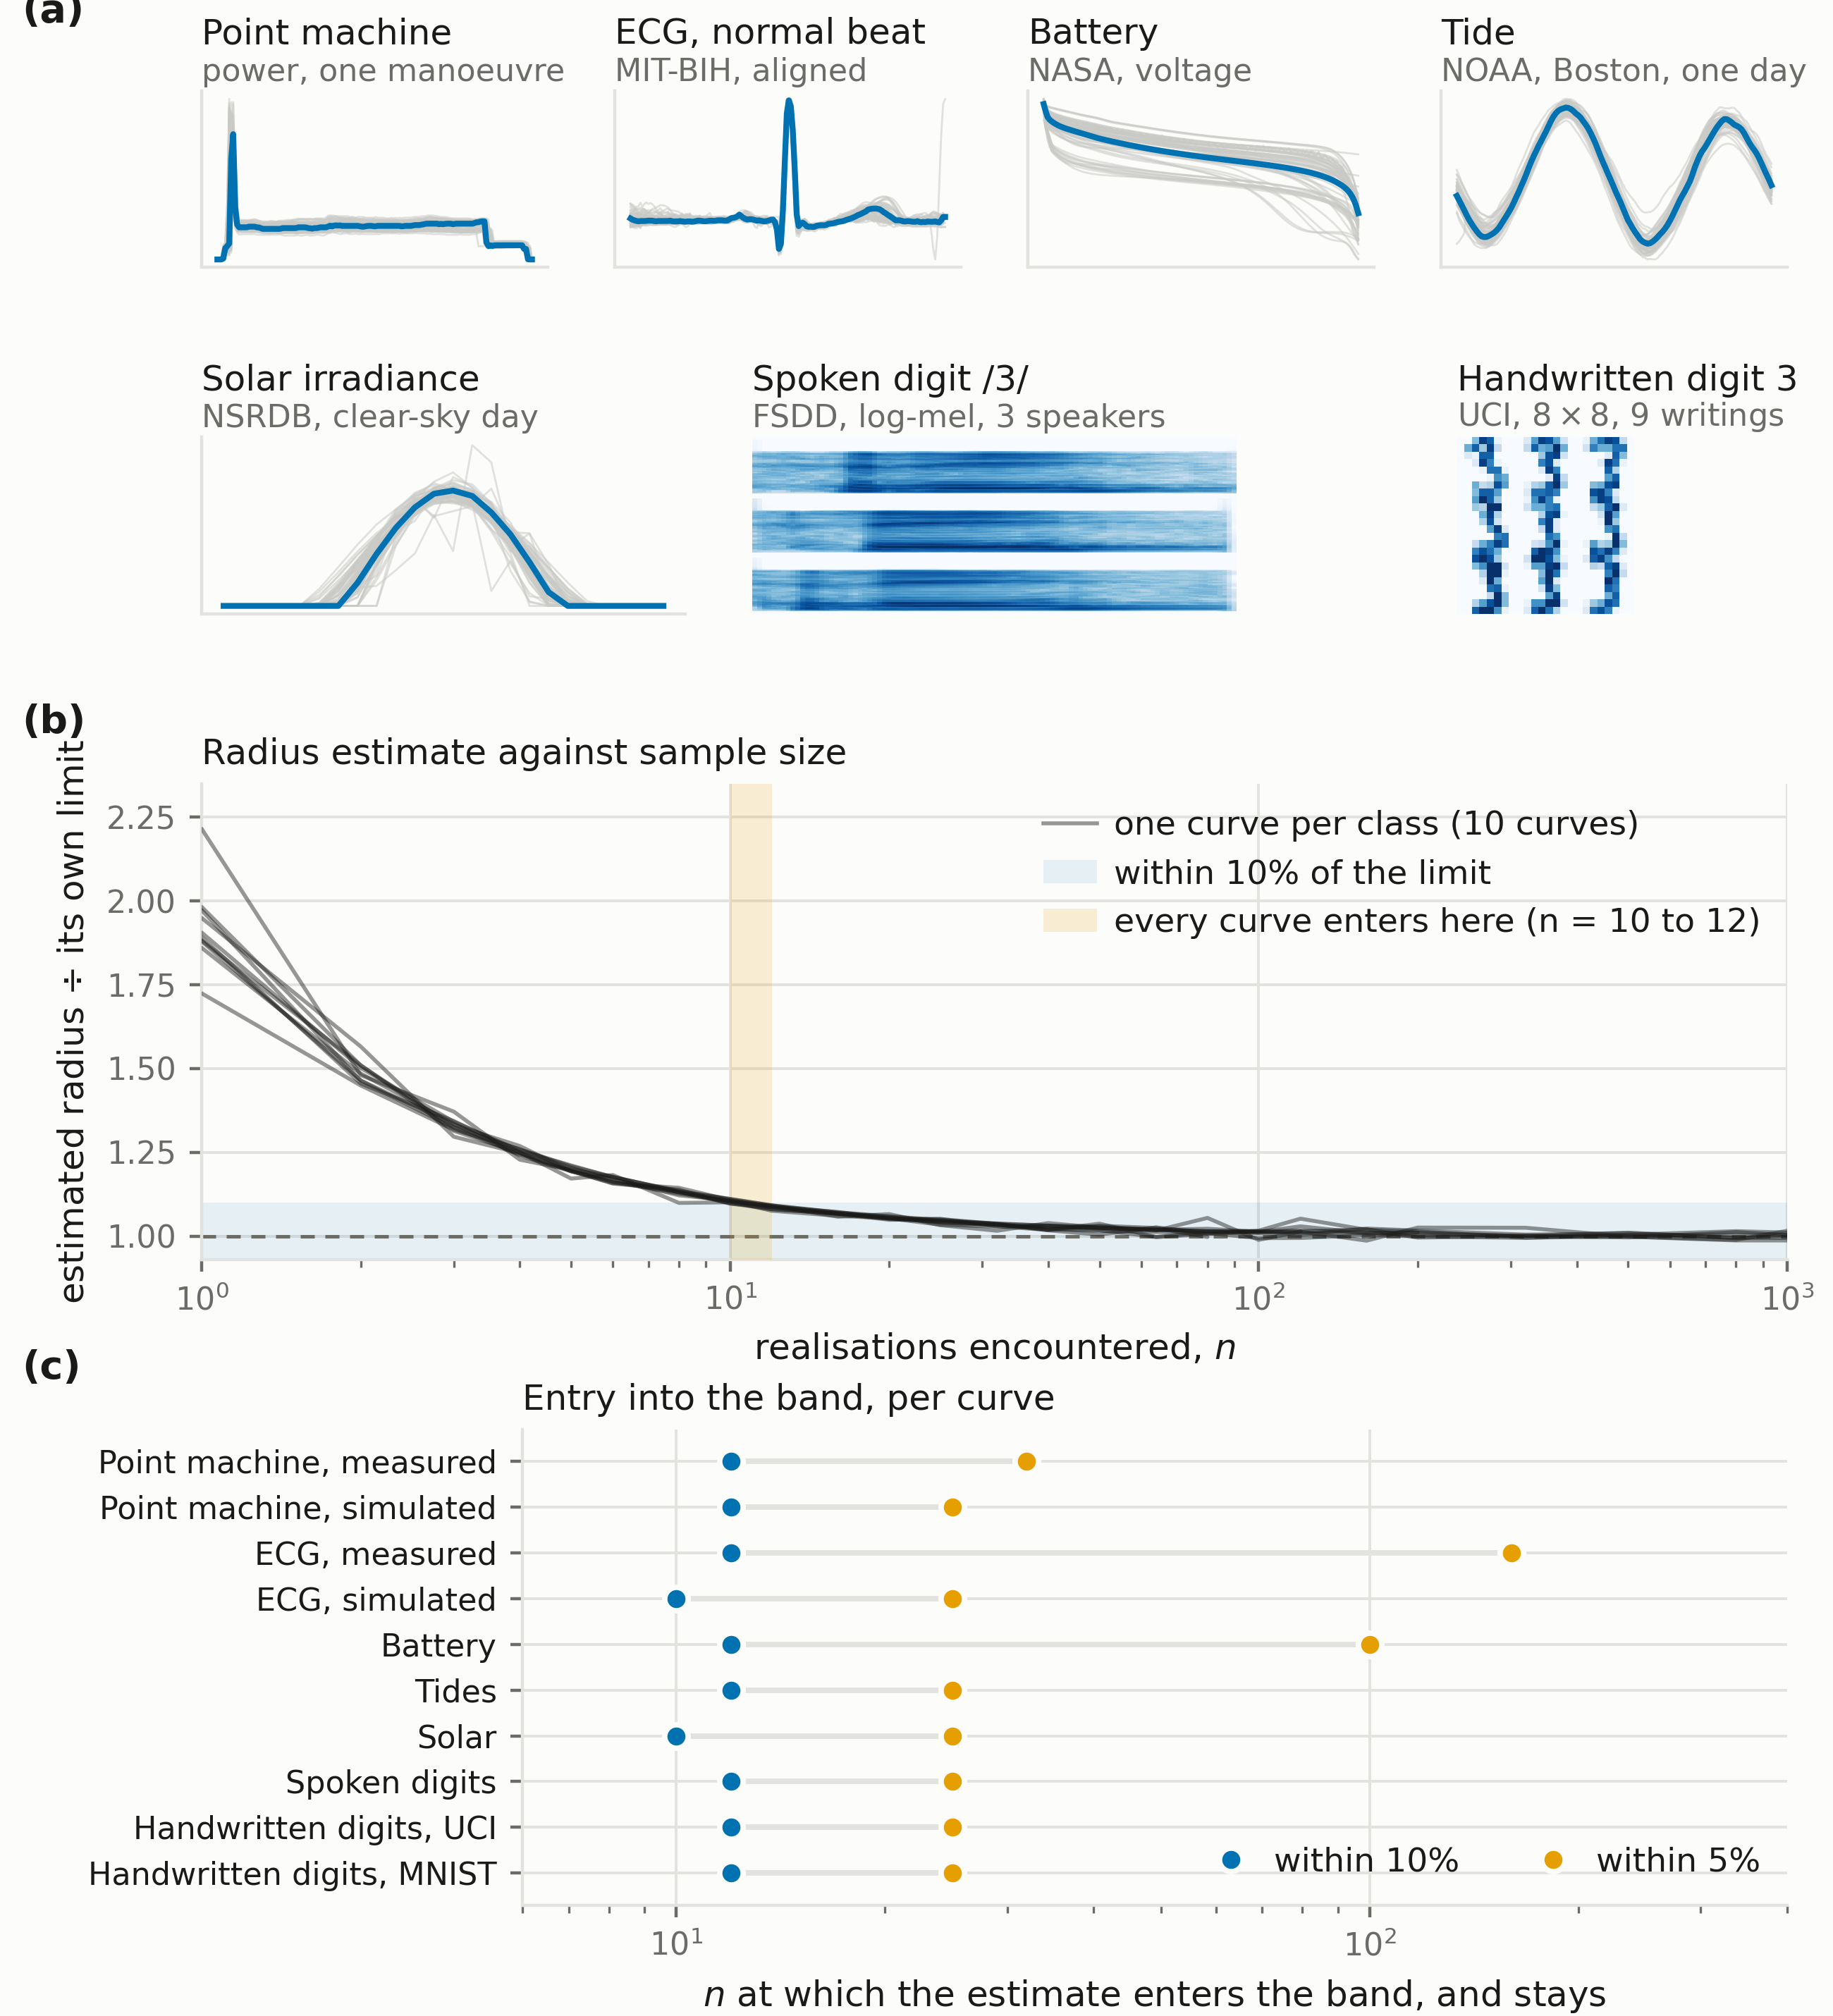
\includegraphics[width=\textwidth]{fig1_seven_phenomena.png}
\caption{\small\textbf{Ten convergence curves over seven phenomena.}
\textbf{(a)} One concept from each of the seven phenomena measured in this
paper: sixty realisations in grey, the medoid in blue, and for the two image
domains three and nine realisations respectively. Nothing is aligned or
selected beyond what the corresponding stage of the reproduction package
already does.
\textbf{(b)} For each of the ten concept sets, the radius an observer
estimates from $n$ encounters --- measured on realisations it has not seen ---
divided by that concept's own limiting radius. Dividing by the limit is what
places ten quantities with ten different units on one axis; it does not
change the shape of any curve. The band is $\pm$10\% of the limit, and the
vertical strip marks the interval within which every curve has entered it.
\textbf{(c)} The value of $n$ at which each curve enters its limit and does not
leave again, at two tolerances.
The claim the figure carries is the one in the text: the estimate stabilises rapidly,
and it does so at a comparable order of $n$ across phenomena that share no
mechanism.}
\label{fig:overview}
\end{figure}

In deterministic systems, repeated measurements do not span an unbounded space of
possibilities; rather, they concentrate within a low-variability structure in
functional space. Factoring out benign variation isolates a distinct set, and a
perceptual category is formally defined by this set rather than by an arbitrary
collection of samples. Once a system has covered this set at its intrinsic
resolution, it can classify a novel realisation by its proximity to the established
covering---and even near the boundaries, it retains a graded, geometric measure of
certainty.

If a perceptual category constitutes a compact set of admissible realisations, the
sensory layer of a perceiving system can be modeled as covering that set, rather
than merely approximating a probability distribution over it. This geometric
description does not impose a specific mechanistic architecture: akin to a delay
embedding, it defines the preserved structure while remaining agnostic
to the underlying implementation.

Throughout this work, $\mathcal{M}$ denotes the set of realised signals
generated by the physical system---the observed perceptual manifold---rather
than the full sensory space.
When the governing equations are unknown, both the manifold structure and its
radius must be inferred directly from the stream of observations, leading
naturally to a self-supervised formulation.
This view is consistent with contemporary approaches to autonomous intelligence
\citep{lecun2022path}, which emphasise that learning arises from discovering the
set of admissible representations produced by the world rather than from
external supervision.

A clarification on terminology is useful at the outset. Throughout this paper,
the term \emph{manifold} is used in the empirical representation-learning
sense of a structured, low-variability subset of a functional space. What is
established here is empirical: how small these subsets are and how quickly an
observer's estimate of that size settles. Compactness and boundedness are
assumed rather than established, and none of it requires the subset to be a
smooth differentiable manifold. Similarly, the structural features discussed
below---such as peaks, plateaus, slopes, transients, and characteristic
morphologies---are treated as stable functional or morphological identifiers,
not as formal topological invariants in the sense of homology, Betti numbers,
or persistent homology summaries.

\subsection{The reference the measurement needs}

Because theoretical finiteness provides weak guarantees, our empirical measurements
rely on relative controls rather than absolute magnitudes. Three baseline
comparisons are employed throughout this study:

First, we compare against \textbf{surrogates} to determine precisely which
structural properties are being compressed. Three surrogate models systematically
destroy the waveform while preserving progressively more of the signal's
statistical properties: a random permutation destroys all temporal structure
including the spectrum; a phase-randomised surrogate preserves the exact power
spectrum \citep{theiler1992surrogate}; and an iterative amplitude-adjusted
surrogate preserves both the power spectrum and the amplitude distribution
\citep{schreiber1996improved}.

Second, we compare against an \textbf{arbitrary class} to verify that the
covering number sees a concept at all, rather than
merely reflecting mathematical boundedness.

Third, we compare against a \textbf{declared invariance} to assess whether
embedding a formal transformation model of the phenomenon alters its empirical
learning complexity.

\subsection{Scope}
\label{sec:scope}

This paper does not propose a mechanistic theory of perception. Its focus is not
the perceiver, but the perceived: the intrinsic structure of the signal families
that any perceiving system encounters. We measure a fundamental property of these
families---specifically, the number of realisations required for their geometry to
stabilise---without invoking an observer model, supervised training, or semantic
labels. Whether and how a biological or artificial perceiver exploits this
structure is a distinct question beyond the scope of this work. Our core claim is
that this structure exists, and it is sufficiently compact to be leveraged.

Our framework operates under a condition narrower than strict determinism, one
that is falsifiable within each domain: the phenomenon's benign variation must
constitute a \textbf{declarable group}. When a sensor measures a physical quantity,
and the transformations preserving the underlying latent state (e.g., gain, offset,
    time origin, duration) can be explicitly formulated, the representation costs nothing.
    Where such a group cannot be formulated, the invariances must instead
    be learned.

This condition formally distinguishes domains that are often colloquially grouped
together. For instance, a class of handwritten digits represents a single abstract
symbol subjected to a group of spatial transformations; consequently, the class
forms an \emph{orbit}. Conversely, a class of natural photographic images forms a
\emph{semantic category}: distinct physical objects that share a linguistic label,
devoid of any formal transformation mapping one to another, and captured via a
3D-to-2D projection that irreversibly destroys information rather than acting on it.
Phenomena such as occlusion and background clutter are not group actions and cannot
be quotiented out. This distinction represents a difference in kind, rather than
merely in difficulty.

The scope of this condition is substantial: a calibrated sensor monitoring a physical
system where nuisance variables are restricted to gain, speed, and offset represents
    the standard paradigm in condition monitoring. In such settings, the cost of perception is lowest,
    as the robust representation is provided intrinsically by
    the instrumentation rather than learned extrinsically from large datasets.

\subsection{Contributions}

\begin{enumerate}
  \item \textbf{Rapid Stabilisation of Geometric Estimates.} The number of
    realisations an observer requires to stabilise its estimate of the geometry of a class is measured
    rather than assumed. Across ten convergence curves spanning seven phenomena
    that share no underlying mechanism, the estimated radius, evaluated on held-out
    realisations, enters and remains within ten per cent of its limit after ten
    to twelve observations. This convergence schedule characterises the observer's sampling
    cost; the property intrinsic to the phenomenon is the geometric size at which the
    estimate settles (Contribution~2). The stabilisation concerns the bulk of the
    class only; its boundary exhibits no comparable convergence
    (Contribution~4).
  \item \textbf{Structural Localisation via Surrogate Controls.} Real physical
    processes can be covered by four to twenty-one exemplars at their intrinsic
    resolution. We isolate whether this low covering number stems from the underlying
    phenomenon or the chosen representation by substituting each signal with a
    surrogate that preserves the power spectrum and amplitude distribution but
    randomises phase relations. In the electromechanical, physiological, and
    electrochemical domains, the covering number is multiplied by a
    factor of $25$ to $149$, so the low covering number is attributable to the phenomenon. Conversely, in the tidal domain, the factor
    is $1.4$, indicating that the distinguishable structure
    is already captured by second-order statistics and amplitude distributions.
    Thus, the surrogate serves as a diagnostic tool for the generative nature of
    the phenomenon, rather than a metric for data compression.
  \item \textbf{Alignment Between Covering Number and the Underlying Concept.} The
    covering number reflects meaningful structure, not merely mathematical
    boundedness: a real class requires between $1.3$ and $3.8$
    times fewer exemplars than an arbitrary class of equivalent size and resolution,
    as verified across three digit datasets at five distinct resolutions.
  \item \textbf{Divergent Convergence Dynamics Between Bulk and Boundary.} The
    within-class median acts as a functional of the measure and stabilises after
    a small number of encounters. In contrast, the maximum distance acts as a
    functional of the support and exhibits no guaranteed rate of convergence. Core
    concepts reside in the interior of the manifold, explaining their high sample
    efficiency.
  \item \textbf{Declared Invariances Directly Drive Sample Efficiency.} Formally
    declaring the benign transformation group reduces the number of samples required
    to achieve a target accuracy by a factor of two to thirty-two across three
    independent readout mechanisms. Furthermore, this efficiency multiplier scales
    with the demanded accuracy: on MNIST, the reduction factor is $2$ to $8$ for
    $85\%$ accuracy, and $4$ to $32$ for $90\%$ accuracy. Conversely, failing to
    declare these invariances incurs steep costs. For instance, in the spoken-digit
    domain, early iterations zero-padded recordings to a fixed length, rendering
    over half of each vector a shared constant. Formally quotienting by duration---the
    standard procedure applied to the physical domains---improved the covering-number
    ratio at the coarsest resolution from $1.05$ to $1.27$, elevated the attainable
    one-class $F_1$ score from $0.57$ to $0.81$, and the exemplars a nearest-neighbour
    readout needs for $95\%$ accuracy from beyond that readout's reach to
    $160$ per class. It leaves the convergence curve exactly where it was.
    That correction was made after those numbers had been seen, and
    Section~\ref{sec:spoken-duration} states what it was, why it is not a choice made
    by inspecting the outcome, and where the uncorrected arm is reported.
  \item \textbf{A Priori Specification of Operating Points.} The error tolerance is
    a parameter chosen by the observer; thus, the memory capacity required to
    achieve a demanded precision can be determined in advance, up to the theoretical
    ceiling of the employed classification rule.
\end{enumerate}

\subsection{Limits and consequence}

This paper does not propose a novel algorithm for perception, a procedure for
unsupervised discovery of the benign transformation group, or a model governing the
transition boundaries between concepts. The $\varepsilon$-net is utilised strictly
as an analytical instrument to measure the geometric class, not as an operational
rule for exemplar selection or as a state-of-the-art classifier. We explicitly
declare the invariance groups and measure the empirical consequences of both
accurate and flawed declarations. Furthermore, the precise boundaries where two
admissible sets intersect---representing inherent ambiguities in the physical
phenomenon---are outside the scope of our geometric modelling.

The practical implications of these findings are specific and immediate. Practitioners
deploying sensors on novel industrial machinery, physiological patients, or
environmental stations must currently rely on heuristics to determine how much
nominal baseline data is required to establish a reliable reference. This work
demonstrates that this requirement need not be guessed; it can be formally and
predictably measured directly from the physical process itself. The current
paradigm in artificial intelligence relies on scaling laws and large datasets,
while biological intelligence exhibits remarkable sample efficiency; whatever
else accounts for that gap, part of it is that the families of signals the world
presents are far smaller than the spaces they live in, and this paper measures
how much smaller.

\section{Related Work}
\label{sec:related}

This paper evaluates the covering number of empirical datasets as a direct
measure of their representational budget. Four distinct bodies of literature
intersect with this proposition, though none addresses it entirely:
the mathematics of metric entropy, which supplies the quantity; the geometry of
perceptual manifolds, which studies the same object along a different axis;
the theory of invariance and sample complexity, which explains why quotienting
by a group should be cheap; and topological data analysis, which asks a
different question about the same point clouds. We state what each contributes
and where our claim sits relative to it.

\subsection{Covering numbers and metric entropy}
\label{sec:rw-covering}

While the mathematical formulation of the covering number is standard, our
empirical interpretation as a representational budget is novel. The
$\varepsilon$-entropy of a set in a function space --- the logarithm of the
smallest number of $\varepsilon$-balls that cover it --- was introduced by
Kolmogorov and Tikhomirov \citep{kolmogorov1993entropy}, who computed it for
the classical function classes and made it the standard measure of the size of
a set in a function space --- the size that matters being this count, not the
ambient dimension. That a totally bounded set has a finite such count at every
resolution is immediate from the definition, and it is the step our
Section~\ref{sec:hypotheses} leans on. Dudley
\citep{dudley1967sizes} tied metric entropy to the continuity of processes on
the set, and the quantity has since become the standard currency of statistical
learning theory, where covering numbers and their combinatorial relatives
control uniform convergence \citep{vapnik1971uniform} and appear directly in
generalisation bounds \citep{cucker2001mathematical, zhou2002covering}; modern
treatments are given by \citet{vershynin2018high} and by
\citet{shalevshwartz2014understanding}.

In that literature the covering number is an intermediate object. It is
bounded, not measured; it is bounded for a \emph{hypothesis class} chosen by
the modeller, and it is used to bound the error of a learner. The move here is
to take the same quantity, compute it for the \emph{data} rather than for a
hypothesis class, on realisations of a physical process rather than on a
function class chosen for its analytic convenience, and report its value rather
than its order of growth. Classical theory guarantees only that this metric
entropy is finite. It does not bound the absolute magnitude---providing no
distinction between a covering number of four or four billion. Resolving this
magnitude empirically forms the core contribution of the subsequent sections.

\subsection{The geometry of perceptual manifolds}
\label{sec:rw-manifolds}

The closest prior geometry is the theory of perceptual manifolds developed by
\citet{chung2018perceptual} and extended to deep
networks by \citet{cohen2020separability}. There a class is
likewise a set rather than a point cloud of independent samples, and it is
characterised by an effective radius and an effective dimension. The axis of
that work is \emph{separability}: given manifolds of a certain radius and
dimension, how many of them can a linear readout separate, and how does a deep
network reshape them so that more can be. The capacity so defined is a property
of the pair (geometry, readout), and the geometry enters as a given.

The axis here is complementary and, as far as we know, not addressed there: not
how many manifolds a readout separates, but how many realisations of one fix
its geometry, and how much of the ambient space that geometry then occupies.
These two frameworks interrogate the same object but address complementary
aspects: a class may be easily separable from others yet remain expensive to
completely characterise. The cost of this characterisation is the
geometric metric most relevant to deploying robust sensory systems. Two
consequences follow from the difference. First, our measurement needs no
readout, no labels and no training, so it can be made before a model exists
rather than after one is fitted; Section~\ref{sec:results-digits} reports both
quantities on the same data and finds them dissociated. Second, while the
manifold-capacity literature typically treats geometry as a property of a
\emph{representation}---tracking its evolution across neural network layers
\citep{cohen2020separability, ansuini2019intrinsic}---our framework posits that,
under a properly declared observable, geometry is an intrinsic property of the
\emph{phenomenon} itself. It represents the underlying structure that learning
algorithms attempt to capture, and it can be measured directly without them.

\subsection{Invariance, quotients and sample complexity}
\label{sec:rw-invariance}

Our fifth contribution---that explicitly declaring and quotienting by a benign
invariance group is what makes a class cheap, and that this saving is
quantifiable---intersects with a literature rich in theory but relatively sparse
in empirical application. The foundational engineering intuition is well-established: tangent distance and tangent propagation
build a declared transformation group into the metric and into training so the
model need not learn it from examples \citep{simard1998transformation}. Mallat's
scattering transform makes the construction exact, producing representations
provably invariant to a compact group and stable to small deformations
\citep{mallat2012group, bruna2013invariant}, and Anselmi et al.\ argue on that
basis that invariance is the property that reduces the sample complexity of
recognition \citep{anselmi2016unsupervised}. Group-equivariant architectures
\citep{cohen2016group} and the geometric-deep-learning programme that
generalises them \citep{bronstein2021geometric} take the same principle as a
design rule, and the theoretical side has since made the benefit quantitative:
generalisation bounds that improve with the size of the invariance group
\citep{sokolic2017generalization, bietti2019group}, a strict generalisation gap
in favour of equivariant models \citep{elesedy2021provably}, data augmentation
analysed as averaging over a group action
\citep{chen2019grouptheoretic}, and, for kernel regression, an exact
characterisation of the sample-complexity gain an invariance buys
\citep{tahmasebi2023exact}.

That body of work says what a declared invariance is worth to a \emph{learner},
in the units of a generalisation bound, and almost always for a hypothesis
class rather than for data. We complement this by characterising the
\emph{object} itself, providing a direct metric of structural complexity. Section~\ref{sec:quotient}
declares a quotient in each domain, measures the covering number with and
without it, and reports the ratio: the cost of refusing to compare two
realisations that the declared group says are the same. The quantity is a
number of exemplars, not a bound; it is measured on the phenomenon before any
model is chosen; and where the declared group is wrong the measurement says so,
because the quotient then fails to shrink the class. This is also where the
scope condition of Section~\ref{sec:scope} comes from and why we state it as
sharply as we do: the account applies where a class is an orbit under a
declarable group, which is exactly the regime these papers assume and rarely
test.

\subsection{The manifold hypothesis, its support, and its dimension}
\label{sec:rw-manifold-hypothesis}

That high-dimensional data lie near a low-dimensional set is old as an
assumption \citep{tenenbaum2000global, bengio2013representation} and
comparatively recent as a testable statement: Fefferman, Mitter and Narayanan
\citep{fefferman2016testing} give an algorithm, with sample complexity, for
deciding whether a distribution is well fitted by a manifold of bounded volume
and reach. The geometric question posed in this work is formally weaker and
computationally more tractable. We do not test whether the admissible set is a
manifold --- Section~\ref{sec:introduction}
says explicitly that we do not need it to be --- but measure the covering
number of the set that the observations exhibit, at a resolution the observer
declares.

Two neighbouring literatures supply the quantities we report. Estimating the
support of a distribution from samples is classical
\citep{devroye1980detection, scholkopf2001estimating}, and the distinction it
makes between the bulk of a class and its boundary is the one that reappears in
our fourth contribution: support functionals are exactly the ones that keep
moving as the sample grows, which is what Section~\ref{sec:bulk-boundary}
measures rather than assumes. Intrinsic dimension has standard estimators,
maximum-likelihood \citep{levina2004maximum} and nearest-neighbour ratio
\citep{facco2017twonn} among them, and has been measured for natural images and
for the representations networks build of them
\citep{pope2021intrinsic, ansuini2019intrinsic}; we report a covering-number
slope instead, for the reason given in
Section~\ref{sec:dimension-protocol}, and calibrate it against sets whose
dimension is known rather than trusting it in the abstract. While intrinsic dimension and the covering number are related, they are not
interchangeable. This distinction is critical for our framework: dimension is an
exponent, whereas the covering number provides an absolute count, which maps
directly to an empirical representational budget.

\subsection{Topological data analysis}
\label{sec:rw-tda}

There is an established programme for extracting topology from finite samples,
and our work is not part of it. Persistent homology tracks the Betti numbers of
a filtration of balls around a point cloud and reports the features that
survive across scales \citep{carlsson2009topology, edelsbrunner2010computational,
chazal2021introduction}; Niyogi, Smale and Weinberger
\citet{niyogi2008finding} give the sampling conditions under which the homology
so recovered is that of the underlying submanifold. The object of study is the
same --- a finite sample of a set in a metric space, examined at a range of
scales. However, we explicitly clarify this distinction to preempt expectations
of persistent homology barcodes where we report convergence curves.

Persistent homology quantifies the \emph{shape} of the data: how many components, loops and voids
the set has, and at which scales they are real. In contrast, we quantify its \emph{size}:
how many balls of a stated radius it takes to cover the set, and how many
realisations an observer needs before that count stops moving. Homology is
invariant to deformations that change a covering number, and a covering number
does not report whether the set it covers has a hole, so neither quantity
determines the other. They also differ in what they need: persistence needs conditions on
reach and sampling density to certify its answer \citep{niyogi2008finding},
where a covering number at a declared resolution needs only the metric.
Applying persistence to the classes measured here --- asking whether these
regions are simply connected, and whether the answer separates domains that our
counts do not --- is a question we have not asked and think worth asking.

\subsection{Domains and analytical instruments}
\label{sec:rw-domains}

Each of the physical domains possesses a mature applied literature focused on diagnosis, anomaly detection, or predictive maintenance \citep{li2020pointmachine, MITBIH_dataset_1980, saha2007prognostics}. These literatures measure decision rule performance on large corpora, but they do not measure the geometric size of the nominal class nor the minimal sampling budget required to characterise it. We use these standard datasets exclusively to test this unexamined geometric property. As analytical instruments, we adopt established methods strictly as baselines: iterative amplitude-adjusted surrogates \citep{schreiber1996improved} for structural evaluation, and nearest-neighbour classification \citep{cover1967nearest} to test the resolving power of the discovered geometry. What is novel is not the decision rule, but demonstrating that a class requires very few prototypes and that they can be selected via uniform random sampling.

\subsection{Where this leaves the contribution}
\label{sec:rw-position}

Positioned against these five literatures, the central claim of this paper remains
narrow and unoccupied. We adopt the covering number metric and its
finiteness guarantee from metric entropy, providing the missing empirical
measurements. We shift the focus of perceptual manifold theory from linear
separability to characterisation cost. We translate the theoretical bounds of
invariance literature into empirical measurements of intrinsic structural complexity.
We adopt a weaker assumption than the strict manifold hypothesis, and we bypass
topological data analysis entirely, as we are concerned with geometric size rather
than topological shape. Finally, we leverage the datasets established by applied
domain literatures to test these geometric properties.

Joint Embedding Predictive Architectures are the nearest thing in current
practice to a system that behaves as though the account here were true. They
learn by predicting latent embeddings rather than reconstructing raw data
\citep{lecun2022path, assran2023self}, and recent vision--language
instantiations predict continuous target text embeddings from visual inputs and
textual queries, matching or exceeding token-generative models under comparable
training conditions \citep{chen2025vljepa}. What none of that work provides is a
characterisation of the geometry that makes prediction in a latent space
feasible in the first place --- the reason a small, continuous target space
exists to predict into. That characterisation is the subject of this paper, and
Section~\ref{sec:discussion} returns to the connection.

% ============================================================
% 2. DETERMINISTIC SYSTEMS AND PERCEPTUAL STRUCTURE
% ============================================================
\section{Deterministic Systems and Perceptual Structure}
\label{sec:deterministic}

\subsection{Deterministic signal generation}

Let a physical system produce outputs $x(t)$ through a deterministic mapping
\[
x = f(s,\theta),
\]
where $s$ represents the internal physical state of the system and $\theta$ 
represents external conditions. Each realised signal $x(t)$ belongs to the 
Banach space $C^0([0,T])$ endowed with the supremum norm. Small perturbations,
manufacturing tolerances, and environmental variations are assumed bounded and 
preserve continuity.

We define the \emph{perceptual set} produced by the system:
\[
\mathcal{M} = \{\, f(s,\theta) : s\in\mathcal{S},\;\theta \in \Theta \,\}
\subset C^0([0,T]).
\]

\subsection{Three hypotheses, and what they are worth}
\label{sec:hypotheses}

The subsequent analysis depends on three foundational properties. These are
empirical conditions concerning the physical processes under observation, which
are stated before anything is measured, and each of them can fail in a given domain.

\begin{description}
  \item[\textnormal{\textbf{H1 (Boundedness).}}] The realisations are uniformly
    bounded. Physically: the measured quantity has limits the process does not
    exceed.
  \item[\textnormal{\textbf{H2 (Equicontinuity).}}] The family is equicontinuous.
    Physically: the rate of change is bounded --- by inertia, by finite power, by
    finite bandwidth.
  \item[\textnormal{\textbf{H3 (A resolving observable).}}] The declared
    observable separates the states the process distinguishes.
\end{description}

Assuming H1 and H2 hold, the finiteness of the covering number follows
immediately from classical analysis. By the Arzel\`a--Ascoli theorem, a
uniformly bounded, equicontinuous family is relatively compact. Because a
relatively compact set is totally bounded, its covering number is guaranteed
to be finite at every resolution.

However, classical analysis does not provide the two quantities evaluated in
this study. First, it does not bound the absolute \emph{magnitude}---the finite
covering number could theoretically be astronomical, yet empirically we find
counts as low as four to twenty-one. Second, it does not determine the
\emph{sampling cost}: the number of realisations required to accurately
estimate this geometry is a statistical property of the estimator, not an
analytical property of the set. Thus, while analysis guarantees finiteness,
only empirical evaluation can establish its magnitude. The validity of these
results ultimately depends on hypotheses H1, H2, and H3, which we evaluate
individually for each domain in Section~\ref{sec:hypotheses-per-domain}.

For a deterministic system on an invariant set of dimension $d$ and a generic
observation function, Takens's theorem establishes that the delay map into
$\mathbb{R}^{2d+1}$ is an embedding \citep{takens1981detecting, sauer1991embedology}.
This implies that a resolving observable generically exists, providing a strong
theoretical motivation for H3. However, two limitations apply. First, these
theorems primarily concern attractors of autonomous systems, whereas several
phenomena evaluated here (e.g., battery discharge, a railway switch maneuver, a
heartbeat) represent transients. Second, genericity guarantees existence but is
not constructive. Consequently, we must explicitly declare the selected observable
for each domain and empirically evaluate its resolving power.

\subsection{Compactness of the perceptual set}

A central premise of this work is that deterministic physical systems generate
signals that occupy a compact region of function space. This property is what
enables generalisation from sparse observations.

\begin{theorem}[Relative compactness of deterministic signals]
\label{thm:compactness}
If the family $\{f(s,\theta)\}$ is uniformly bounded and equicontinuous on
$[0,T]$, then the perceptual set $\mathcal{M}$ is \emph{relatively compact} in
$C^0([0,T])$: its closure $\overline{\mathcal{M}}$ is compact, and
$\mathcal{M}$ is totally bounded. In particular its covering number
$N(\mathcal{M},\varepsilon)$ is finite for every $\varepsilon > 0$.
\end{theorem}

\noindent Proof: See \ref{app:proofs}.

This follows from the Arzel\`a--Ascoli theorem \citep{royden2010real,
rudin1991functional, conway1990course} under hypotheses H1 and H2. The theorem
establishes relative compactness: the set $\mathcal{M}$ is totally bounded,
which is sufficient to guarantee a finite covering number at any resolution
without requiring $\mathcal{M}$ to be closed. Consequently, the system cannot
produce arbitrary variability; all realised signals are confined to a bounded,
finite-variability region of function space that can be covered by a finite
number of exemplars. (Where a subsequent measurement requires a maximum rather
than a supremum, it is evaluated on the closure $\overline{\mathcal{M}}$; the
value of the supremum remains identical by continuity and density).


Figure~\ref{fig:perceptual_manifold} provides a schematic representation of
this geometric constraint: a set of admissible realisations confined within a
closed ball in $C^0([0,T])$. The figure is purely illustrative, depicting the
geometry implied by relative compactness; all empirical measurements are reported
in Figure~\ref{fig:overview} and subsequent tables.

\begin{figure}[!htbp]
\centering
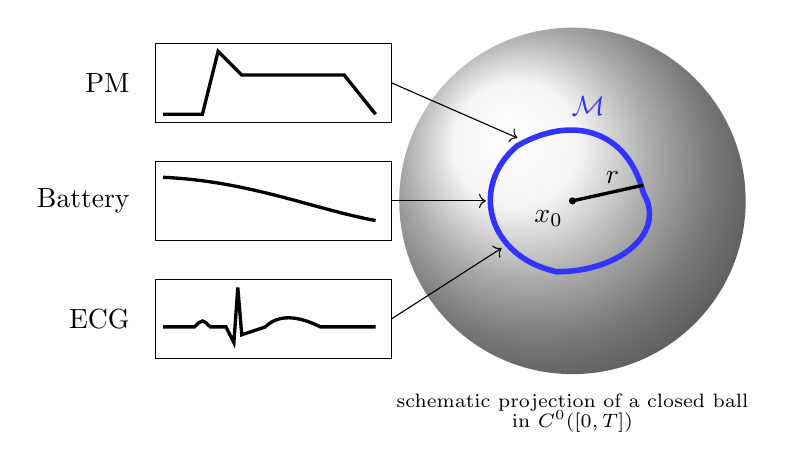
\begin{tikzpicture}[x=1cm,y=1cm]

%--------------------------------
% Left column: mini-plots
%--------------------------------

\tikzset{mini plot/.style={draw=black, very thin, minimum width=3cm, minimum height=1cm}}

% --- PM mini-plot (idle – inrush – locking – idle) ---
\begin{scope}[shift={(-4,1.5)}]
  \node[mini plot, anchor=west] (pmframe) at (0,0) {};
  \begin{scope}[shift={(0,-0.5)}]
    \clip (0,0) rectangle (3,1);
    \draw[very thick]
      (0.1,0.1) -- (0.6,0.1)
      -- (0.8,0.9)
      -- (1.1,0.6)
      -- (2.4,0.6)
      -- (2.8,0.1);
  \end{scope}
  \node[anchor=east] at (-0.2,0) {PM};
\end{scope}

% --- Battery mini-plot ---
\begin{scope}[shift={(-4,0)}]
  \node[mini plot, anchor=west] (batframe) at (0,0) {};
  \begin{scope}[shift={(0,-0.5)}]
    \clip (0,0) rectangle (3,1);
    \draw[very thick]
      (0.1,0.8) .. controls (1.2,0.75) and (2.0,0.4) .. (2.8,0.25);
  \end{scope}
  \node[anchor=east] at (-0.2,0) {Battery};
\end{scope}

% --- ECG mini-plot ---
\begin{scope}[shift={(-4,-1.5)}]
  \node[mini plot, anchor=west] (ecgframe) at (0,0) {};
  \begin{scope}[shift={(0,-0.5)}]
    \clip (0,0) rectangle (3,1);
    \draw[very thick]
      (0.1,0.4) -- (0.5,0.4)
      .. controls (0.6,0.5) .. (0.7,0.4)
      -- (0.9,0.4) -- (1.0,0.2)
      -- (1.05,0.9)
      -- (1.1,0.3)
      -- (1.4,0.4)
      .. controls (1.6,0.6) and (1.9,0.5) .. (2.1,0.4)
      -- (2.8,0.4);
  \end{scope}
  \node[anchor=east] at (-0.2,0) {ECG};
\end{scope}

%--------------------------------
% Right column: schematic ball + manifold
%--------------------------------

\begin{scope}[shift={(1.3,0)}]

\shade[ball color=gray!10, opacity=1] (0,0) circle (2.2);

% Single closed manifold curve (schematic projection)
\draw[blue!80, line width=2pt]
  (0.9,0.1)
    .. controls (0.7,0.9) and (0.0,1.1) ..
  (-0.7,0.7)
    .. controls (-1.3,0.2) and (-1.1,-0.7) ..
  (-0.2,-0.9)
    .. controls (0.6,-0.9) and (1.2,-0.4) ..
  (0.9,0.1);

\fill (0,0) circle (1.3pt);
\node[anchor=north east] at (0,0) {$x_0$};

% Radius to a point on M
\draw[very thick] (0,0) -- (0.9,0.2);
\node[anchor=south west] at (0.3,0.1) {$r$};

\node[blue!80] at (0.2,1.2) {$\mathcal{M}$};

\node[font=\scriptsize, align=center] at (0,-2.7)
{schematic projection of a closed ball\\[-0.1em] in $C^0([0,T])$};

\end{scope}

%--------------------------------
% Arrows from mini-plots to manifold
%--------------------------------

\draw[->, thin] (-1, 1.5) -- (0.6,0.8);
\draw[->, thin] (-1, 0.0)  -- (0.2,0.0);
\draw[->, thin] (-1,-1.5) -- (0.4,-0.6);

\end{tikzpicture}

\caption{\small
Schematic projection of compact perceptual manifolds in $C^0([0,T])$.
The grey ball is not intended as a Euclidean embedding of the function space,
but as a visual representation of bounded variability: admissible realisations
remain within a finite perceptual radius around a reference signal $x_0$.
Representative physical systems---railway point machines, battery discharge,
and ECG waveforms---generate signals that concentrate on compact,
low-variability subsets. Other deterministic domains studied in this work,
including solar irradiance profiles and tidal cycles, exhibit the same type of
compact, bounded-variability structure under the adopted representation.
}
\label{fig:perceptual_manifold}
\end{figure}

\subsection{Closed-ball structure and stable functional markers}

Compactness implies the existence of a center $x_0 \in \mathcal{M}$ 
and a finite radius $r$ such that:
\[
\mathcal{M} \subset B_\infty(x_0,r)
= \{\,x \in C^0 : \|x-x_0\|_\infty \le r \,\}.
\]

The perceptual radius $r := \sup_{x\in\mathcal{M}} \|x-x_0\|_\infty$ is
necessarily finite, as relative compactness immediately implies boundedness.

This radius represents the intrinsic extent of the phenomenon’s variability.
Within this ball, the system exhibits consistent functional and morphological
structures: peaks, plateaus, slopes, impact transients, or physiological wave
morphology. These structures remain stable across admissible realisations and
therefore serve as operational invariants of the observed process class, in the
sense that they are preserved under the bounded variability generated by the
system.

% ============================================================
% 5. PERCEPTUAL FUNCTIONS AND UNIVERSAL APPROXIMATION
% ============================================================


The classical results used below---including the Universal Approximation Theorem for perceptual functionals and the theoretical bounds for Monte Carlo radius estimation---are detailed in Appendix A.

\section{Empirical Radius and Knowledge Boundaries}
\label{sec:radius-section}


\subsection{The perceptual radius}

Using the Hausdorff metric $d_H$ \citep{edgar2008measure}, the perceptual 
radius is defined as:
\[
r = \sup_{x\in\mathcal{M}} d_H(\{x\}, \{x_0\})
= \sup_{x\in\mathcal{M}} \|x - x_0\|_\infty.
\]

The finiteness of $r$ is an immediate consequence of the uniform boundedness
condition established in hypothesis H1.

\section{Methods}
\label{sec:methods}
Our experimental evaluation follows a unified pipeline applied identically
across every domain studied in this work: the seven phenomena of
Section~\ref{sec:results} and Section~\ref{sec:results-digits}, together with
the two deterministic simulators used as controls on the procedure. The goal is to
estimate the geometry of the perceptual manifold---its compactness, operational
invariants, and empirical radius---from real-world signals without relying on 
domain-specific modelling.

\subsection{Monte Carlo radius estimation}
\label{sec:methods-radius}

To quantify how the perceptual radius evolves as sampling becomes dense, we 
estimate the empirical radius
\[
\hat r_n = \max_{1 \le i \le n} \|x_i - x_0\|_\infty
\]
over randomly drawn subsets of increasing size $n$.  
This procedure provides a nonparametric Monte Carlo (MC) estimator of the 
Hausdorff radius of the perceptual manifold.

Because the perceptual set $\mathcal{M}$ is bounded --- H1, which is also half
of what Theorem~\ref{thm:compactness} needs --- $\hat r_n$ is a monotonically
non-decreasing sequence bounded above by the true radius $r$.  
Thus, as sampling becomes dense in the state--condition space, $\hat r_n$ 
converges to $r$ almost surely (Theorem~\ref{thm:mc}).  
The rate and trajectory of this convergence constitute a primary empirical
contribution of this work. Rapid initial growth reflects the discovery of
frequent variability modes; the subsequent plateau of $\hat{r}_n$ indicates
that the estimate has stabilised at the reported resolution. This stabilisation
is a statistical property of the estimator rather than a certificate that the
absolute extremes of the phenomenon have been observed. This distinction is
quantified in Section~\ref{sec:bulk-boundary}: across identical draws, the
within-class median stabilises rapidly (often by $n=5$), whereas the
within-class maximum continues to approach the theoretical supremum
asymptotically.

Operationally, we compute $\hat r_n$ by repeatedly drawing random subsets of 
size $n \in \{10, 20, 50, \dots\}$, embedding signals in $\mathbb{R}^N$, 
and evaluating their distances to the reference signal $x_0$ under the chosen
operational metric.
No class labels or fitted parametric models are required; the estimator depends
only on the observed signals under the adopted preprocessing and metric protocol,
and therefore reflects the \emph{self-supervised emergence of perceptual structure}
from data.

This MC-based procedure is applied identically to real datasets and to 
synthetic signals generated by the simulator, enabling direct comparison of 
radius saturation and geometric compactness under the same preprocessing and 
metric geometry.


\subsection{Preprocessing and functional normalisation}

All signals are resampled onto a uniform temporal grid in $[0,T]$, detrended
when necessary, and normalised to unit amplitude to enable comparison under a
common representation and scale. No temporal warping, smoothing, or feature
extraction is applied.

\subsubsection{Which quotient, and the evidence for it}
\label{sec:quotient}

Two normalisation quotients are employed in this study. Amplitude scaling alone
($\ell_2$) is appropriate when the zero baseline holds physical significance;
amplitude scaling combined with mean subtraction ($z$-score) is required when
the baseline offset is arbitrary. This choice must be declared according to the
physical properties of each domain rather than applied as a uniform heuristic.
The empirical impact of this choice is quantified in Table~\ref{tab:quotient}.

The necessity of this domain-specific declaration is evident in the battery
discharge dataset. A typical discharge curve comprises approximately $3.3$~V of
DC offset carrying only $0.2$~V of dynamic signal. Under standard $\ell_2$
normalisation without offset removal, every realisation projects to nearly the
same unit vector, yielding a within-class median distance of $0.00027$. At this
scale, the metric resolves numerical precision artefacts rather than
electrochemical dynamics. Removing the baseline offset prior to scaling
($z$-quotient) restores the median distance to $0.02543$, aligning the scale of
variance with the other physical domains. Consequently, battery discharge
requires the $z$-quotient.

The ECG domain provides a contrasting case: the two quotients yield indistinguishable within-class median distances ($0.05035$ versus $0.05030$).
Because R-peak-aligned cardiac beats naturally oscillate around a stable
baseline, the offset is negligible. The railway point-machine data represents an
intermediate case: the offset encodes the steady-state idle power level, and
removing it artificially widens the geometric class by a factor of six.
Separability is largely insensitive to the choice of
quotient across all domains (fluctuating by less than $0.01$). Thus, the
quotient is selected exclusively to ensure the dynamic signal is geometrically
resolved, rather than to optimise a classification metric.

\begin{table}[!htbp]\centering\small
\fitwidth{\begin{tabular}{lrrrr}
\toprule
& \multicolumn{2}{c}{$\ell_2$ (amplitude)} & \multicolumn{2}{c}{$z$ (amplitude + offset)} \\
\cmidrule(lr){2-3}\cmidrule(lr){4-5}
domain & within med. & separab. & within med. & separab. \\
\midrule
PM real (nominal) & 0.05080 & 0.966 & 0.32247 & 0.973 \\
PM simulated & 0.03566 & 0.978 & 0.26104 & 0.980 \\
ECG real (MIT-BIH) & 0.05035 & 0.944 & 0.05030 & 0.944 \\
ECG simulated & 0.08369 & 0.716 & 0.08369 & 0.716 \\
Battery real (NASA) & 0.00027 & 1.000 & 0.02543 & 0.999 \\
\bottomrule
\end{tabular}
}
\caption{\small The two quotients on the physical domains. \emph{within med.} is
the median within-class cosine distance and \emph{separab.} is
$P(d_{\mathrm{within}} < d_{\mathrm{between}})$. The declared choice is $\ell_2$
for the point machine and ECG and $z$ for battery discharge.}
\label{tab:quotient}
\end{table}


For the spoken digits domain, specific padding rules were evaluated to test the robustness of the normalisation. Details and the corresponding room tone experiment are deferred to Appendix~\ref{app:padding}.
\subsection{Intrinsic dimension: protocol and calibration}
\label{sec:dimension-protocol}

Section~\ref{sec:related} noted that intrinsic dimension has standard
estimators --- maximum likelihood \citep{levina2004maximum} and the
nearest-neighbour ratio \citep{facco2017twonn} among them --- and that we report
a covering-number slope instead. The reason is that the covering number is
already the instrument every other measurement in this paper uses, so reporting
its slope keeps one construction rather than importing a second with its own
assumptions. The cost of that choice is that a slope fitted to
$\log |S(\varepsilon)|$ against $\log(1/\varepsilon)$ can be moved by choosing
the range of $\varepsilon$ fitted over. Initial analyses reported
$1.36$ for handwritten digits and, on a different grid, $1.98$: nothing was
wrong with either run, and neither range had been declared. A number a reader
can move by choosing the grid is not a measurement.

The protocol therefore fixes every choice in the open.

\begin{itemize}
  \item \textbf{Metric.} The slope is fitted against the \emph{angular} metric
    $\theta = \arccos(1 - d_{\cos})$, not against cosine distance. Near zero,
    cosine distance is quadratic in angle, so a cosine ball of radius
    $\varepsilon$ is an angular ball of radius ${\sim}\sqrt{2\varepsilon}$, and
    fitting against $\varepsilon$ reports half the dimension. The net is
    untouched: a cosine ball of radius $\varepsilon$ \emph{is} the angular ball
    of radius $\theta(\varepsilon)$, the same points and the same $S$; only the
    abscissa of the fit changes.
  \item \textbf{Grid.} Twelve points, log-uniform in $\varepsilon$, between the
    first and ninetieth percentile of the within-set distance distribution.
    Derived from the data, never guessed.
  \item \textbf{Admissible window.} Fit only where
    $4 \le |S(\varepsilon)| \le n/4$. Below four the net has collapsed to a
    handful of points and the slope is dominated by rounding; above $n/4$ the
    net is running out of \emph{data} rather than of geometry, and the slope is
    biased down. Fewer than four admissible points means the sample cannot
    support the estimate, and we report NA rather than a number.
  \item \textbf{Averaging and fit.} $|S(\varepsilon)|$ is the mean over five
    arrival orders of the greedy net, so the estimate does not depend on the
    order the realisations arrived in; the slope is ordinary least squares,
    reported with its standard error, the number of admissible points, and $n$.
\end{itemize}

The estimator is then calibrated rather than trusted. The identical protocol is
run on uniform samples from spheres $S^d$ embedded in $\mathbb{R}^{64}$ at
matched sample size. It recovers $d=1$ essentially exactly and is increasingly
conservative above it --- the covering number of a $d$-dimensional set grows
like $\theta^{-d}$, so at fixed $n$ the admissible window shrinks as $d$ grows
and the fit is pulled down. Every dimension reported in this paper is therefore
a \emph{lower bound}, and the calibration is printed beside it in
Table~\ref{tab:dimension} so that the reader can see how far it can be trusted.
Two rows of that table sit above the calibrated range and are marked as such;
they should be read as ordinal, not as values.

\subsection{Distance metric and Hausdorff evaluation}

The theoretical framework is formulated in the Banach space $C^0([0,T])$ with 
the supremum norm $\|\cdot\|_\infty$, which induces the Hausdorff metric on 
compact subsets. Accordingly, the theoretical perceptual radius is defined as
\[
r = \sup_{x \in \mathcal{M}} \|x - x_0\|_\infty,
\]
with empirical estimator
\[
\hat{r}_n = \max_{1 \le i \le n} \|x_i - x_0\|_\infty.
\]

In the experiments, signals are discretised into vectors in $\mathbb{R}^N$ and
stored in a vector index for efficient nearest-neighbour queries. After
discretisation and normalisation, we report an analogous operational radius
under cosine distance. We do not identify this quantity numerically with the
continuous supremum-norm radius. Rather, cosine distance is used as a
computationally convenient geometry for comparing normalised signal shapes.

The empirical claim is therefore metric-operational: under a fixed
preprocessing pipeline, representation, normalisation, metric, and sampling
protocol, the observed radius and internal Hausdorff discrepancy exhibit rapid
saturation. This qualitative saturation behaviour is the object of empirical
analysis, while the $C^0$ formulation provides the continuous theoretical
setting in which compactness and finite variability are defined.

\begin{remark}[Practical use of cosine distance]
Although the continuous theory is stated in $C^0([0,T])$ with the supremum
norm, empirical computation requires a finite-dimensional representation.
On finite-dimensional vector spaces, standard norms such as $\ell_2$ and
$\ell_\infty$ are topologically equivalent and therefore preserve compactness
properties. However, this equivalence does not imply metric identity: different
metrics may induce different numerical radii, nearest-neighbour relations, and
local geometries.

For this reason, cosine distance should be understood as an operational metric
on normalised discretised signals, not as a numerical substitute for the
continuous supremum norm. The relevant empirical observation is that radius
saturation appears robust under the adopted representation and metric.
\end{remark}

\subsection{Practical implementation: incremental radius estimation}

In practice, the perceptual radius can be estimated incrementally as new
realisations are observed. After selecting an initial reference trace $x_0$,
each subsequent signal $x_i$ is embedded as a vector in $\mathbb{R}^N$ and
inserted into an approximate nearest-neighbour index. No such index is used
in the measurements reported here, which compare exhaustively; it is named
because the incremental construction is what an implementation at scale would
need, not because this work depends on one.
The empirical radius is updated online as
\[
\hat r_n = \max_{1 \le i \le n} \|x_i - x_0\|_\infty,
\]
computed either explicitly or through stored distances maintained by the index.

A key practical observation is that the perceptual manifold becomes usable
long before the radius fully converges: the internal structure (cluster
stability, operational invariants, neighbourhood relations) stabilises early, while late
samples primarily refine the outer boundary. Thus, anomaly detection,
compatibility scoring, and geometric clustering can be deployed immediately,
even while the empirical outer boundary of the manifold is still being refined.

This incremental process reflects the self-supervised nature of perceptual
structure: the observer expands its approximation of $\mathcal{M}$ simply by
accumulating realisations, without labels or a predefined model of the
underlying physics.

A practical question now arises: \emph{how does an observer determine when its
estimate has stopped moving?} Although the radius $r$ is mathematically
well-defined, in real-world settings it must be inferred progressively as new
realisations are observed. At early stages, observations remain tightly
clustered around the reference $x_0$, yielding a small empirical radius. As
sampling becomes denser, previously unseen regions of the manifold appear and
the estimated radius expands. The question the observer can answer is when
$\hat r_n$ has entered a stated band around the value it converges to and has
not left it again --- the criterion of Section~\ref{sec:crossings}. The question
it cannot answer, and which this paper does not claim to answer, is whether the
support has been exhausted: additional samples do \emph{not} all lie inside the
region already seen, and the rate at which the outermost ones keep appearing is
measured in Section~\ref{sec:bulk-boundary}.

The
empirical radius $\hat r_n$ grows rapidly at first as previously unseen extremal
behaviours are encountered, and then flattens. What flattens is the estimate at
the resolution being read; new samples predominantly, not exclusively, fall
inside the region already seen, and the residual traffic at the edge is what
Section~\ref{sec:bulk-boundary} quantifies.

To formalise this estimation procedure, we compute $\hat r_n$ incrementally as 
new samples arrive. The pseudocode below summarises the algorithm used in all 
experiments, implementing the Monte Carlo estimator of the perceptual radius 
and revealing its convergence as sampling becomes dense in the 
state--condition space.



The
real operational signal of convergence
comes from the evolution of the empirical radius $\hat r_n$ as a function of the
number of observed realisations. 

In deterministic physical systems, new samples initially reveal previously
unseen variability, causing $\hat r_n$ to grow rapidly. However, once the
estimate has absorbed the variability that is common in the class, the radius
enters a plateau regime at the resolution being read: the great majority of
additional realisations fall within the region already seen, and $\hat r_n$
moves by less than the band being quoted. 

This gives a practical, data-driven criterion, and it is worth naming what it
is a criterion for. It marks the point at which the observer's \emph{estimate}
has stopped moving, at a stated tolerance and under the sampled operational
regime, without access to the underlying equations. It does not mark the point
at which the admissible set has been covered. Sampling continues to be
useful past it in two distinct ways: internal structure --- neighbourhoods,
operational invariants, cluster geometry --- keeps being refined, and the
extremes of the set keep arriving, which is the part
Section~\ref{sec:bulk-boundary} shows has no settling rate at all.

What that pattern looks like in each domain is not illustrated here but
measured: Table~\ref{tab:saturation_summary} reports how far the estimate still
sits from its limit at four sample sizes in all ten convergence curves, and
Figure~\ref{fig:overview} shows one concept from each phenomenon beside its own
curve. A preliminary draft of this section carried a schematic curve with
hand-chosen coordinates at this point. It was captioned as conceptual, but the
sentence introducing it called it a curve observed across all datasets, which it
was not; it is removed rather than relabelled.


\begin{remark}[Cross-domain evidence for saturation behaviour]
Across all seven phenomena---electromechanical point machines, electrochemical
battery discharge, physiological ECG morphology, solar irradiance, tides,
handwritten digits and spoken digits---the empirical evolution of 
the perceptual radius exhibits the same characteristic pattern: a rapid initial 
expansion followed by a clear saturation plateau. The recurrence of this pattern across heterogeneous domains is a property of
the observer's estimate. What the underlying physics constrains is not the rate of convergence
but the value at which the estimate settles, which is the subject of the next
paragraph and of Section~\ref{sec:surrogates}.
Real phenomena do not explore the full geometric extent 
permitted by the space (e.g.\ cosine distance approaching~1). Instead, 
physical structure constrains variability to a small region shaped by the 
underlying physics.

Anomalous or non-physical signals can approach the theoretical maximum 
(e.g.\ cosine distance near~1), but nominal realisations never do. Across all 
datasets analysed, the empirical radius settles well below this limit, so the
region these families occupy is a small fraction of what the metric allows. Compactness is not what this shows --- it is assumed, and under H1 and H2 it is
forced. What it shows is that the bounded region these families occupy is a
small fraction of the space the metric allows, which is an empirical magnitude
and does not follow from Sections~\ref{sec:deterministic}--\ref{sec:radius-section}.
\end{remark}
%-------

\subsection{The three hypotheses, domain by domain}
\label{sec:hypotheses-per-domain}
Section~\ref{sec:hypotheses} stated H1, H2 and H3 as claims about the world. A detailed domain-by-domain declaration of these hypotheses is deferred to Appendix~\ref{app:hypotheses}. Table~\ref{tab:hypotheses_summary} provides a compact summary of the observable and the bounds posited for each domain.

\begin{table}[ht]
\centering
\small
\begin{tabular}{p{2.2cm} p{3.8cm} p{3cm} p{2.5cm} p{2.8cm}}
\toprule
\textbf{Domain} & \textbf{Observable} & \textbf{H1 Bounds} & \textbf{H2 Constraints} & \textbf{H3 Weakness} \\
\midrule
\textbf{Railway PM} & RMS power ($n=160$) & Rated motor power & Inertia / induct. & The duration \\
\textbf{ECG} & One beat ($n=160$) & Cardiac potentials & Conduction vel. & Single lead proj. \\
\textbf{Battery} & Terminal voltage & Electrochemistry & Capacitance & Internal state \\
\textbf{Tides} & Water level (lunar day) & Depth \& gravity & Astro. forcing & Spring-neap norm. \\
\textbf{Solar} & GHI over 24h & Extraterrestrial & Cloud edges & Unresolved atmos.\ state \\
\textbf{Audio Digits} & Log-mel spectrogram & Recording floor & Vocal tract & Separability 0.63 \\
\textbf{Image Digits}& Pixel int.\ ($[0,1]$) & By construction & By construction & Concept overlaps \\
\bottomrule
\end{tabular}
\caption{Summary of the structural bounds (H1--H3) across domains.}
\label{tab:hypotheses_summary}
\end{table}

\subsection{Cross-domain evaluation}

The same pipeline (Section~\ref{sec:methods}) is applied to the railway point machine dataset, the NASA 
battery aging dataset, the MIT-BIH ECG database, NSRDB solar irradiance data, and NOAA tidal records. 
Because all domains are processed identically, differences in perceptual 
geometry reflect the underlying physical processes rather than methodological 
bias.

Complete implementation details, including preprocessing scripts, Hausdorff
computations, Monte Carlo sampling, and figure-generation code, are provided in
the public repository associated with this article:
\url{https://github.com/eduardodisanti/shamayam}.

\subsection{Public Datasets and Synthetic Generators}
\label{sec:datasets}

To examine whether deterministic functional topology captures a recurring geometric property, we evaluate the framework across public datasets and synthetic procedural controls. Their configurations are summarised in Table~\ref{tab:datasets_summary}. Detailed generator parameterisations reside in the Appendices.

\begin{table}[ht]
\centering
\small
\begin{tabular}{p{3cm} p{4cm} p{7cm}}
\toprule
\textbf{Domain} & \textbf{Dataset / Source} & \textbf{Characteristics \& Treatment} \\
\midrule
\textbf{Railway PM} & CRPM \citep{li2020pointmachine} & 8788 traces (2 units, 2 directions), pooled together. \\
\textbf{Battery Aging} & NASA Ames \citep{saha2007prognostics} & Constant-current discharge curves. \\
\textbf{ECG} & MIT-BIH \citep{MITBIH_dataset_1980} & Morphological heartbeats (P, QRS, T). \\
\textbf{Solar} & NSRDB \citep{sengupta2018nsrdb} & Hourly GHI profiles split by cloud cover. \\
\textbf{Tides} & NOAA \citep{noaa_coops_tidescurrents} & Lunar-day cycles aligned at high water. \\
\textbf{Digits (Audio)} & FSDD \citep{fsdd} & Log-mel spectrograms, quotiented by duration. \\
\textbf{Digits (Image)} & MNIST \citep{lecun1998mnist}, UCI \citep{uci_optdigits} & $28\times 28$ and $8\times 8$ pixel intensity lattices. \\
\textbf{Synthetic Controls} & Procedural generators & Deterministic bounds by construction (PM and ECG). \\
\bottomrule
\end{tabular}
\caption{Overview of public datasets and synthetic procedural controls.}
\label{tab:datasets_summary}
\end{table}

\section{Results: Geometry Across Domains}
\label{sec:results}

% ------------------------------------------------------------
% 6.1 RESULTS — POINT MACHINE MANIFOLD
% ------------------------------------------------------------
\subsection{Point Machines: Functional Manifold Geometry}

We evaluate whether the instantaneous power envelopes of electromechanical
railway point machines (PMs) form a compact functional manifold and whether
Monte Carlo (MC) simulation can approximate its geometry in the absence of
large real datasets. All signals were normalised in amplitude and resampled to
$160$ points before being compared under cosine geometry, used here as a
finite-dimensional proxy for signal-shape similarity. The resampling is a
quotient by duration, declared in Section~\ref{sec:hypotheses-per-domain}
together with what it costs.


% ------------------------------------------------------------
% 6.1.1 REAL MANIFOLD SATURATION
% ------------------------------------------------------------
\subsubsection{Saturation of the Real PM Manifold}

For a subset $X_n$ of $n$=8788 real signals, we compute:
\[
r_{\max}(X_n), \qquad
\bar{r}(X_n), \qquad
E_{\mathrm{bbox}}(X_n),
\]
where
$E_{\mathrm{bbox}}(X_n) = \sum_j \left( \max_i x_{ij} - \min_i x_{ij} \right)$
is the summed coordinate extent of the sample. It is a bounding-box statistic
but it is not a volume: it is a sum of per-coordinate ranges, not their
product, and it is reported because a product over hundreds of coordinates
underflows to zero and measures nothing.

Of these, the mean radius is the functional of the measure and constitutes the
primary convergence metric evaluated in this study. The maximum and the summed
extent are functionals of the support and are reported without a convergence
claim (Section~\ref{sec:bulk-boundary}). Table~\ref{tab:saturation_summary}
quantifies the former for this domain: the estimated radius converges to within
$5.3\%$ of its limit at $n=20$ and within $0.4\%$ at $n=50$. Applying
the stability criterion of Section~\ref{sec:crossings}---the sample size beyond
which the estimate remains strictly within a stated tolerance---this domain
stabilises within ten per cent at $n=12$, five per cent at $n=32$, and one per cent
only at $n=8000$.

These signals occupy a low-variability region governed by the physical mechanism---motor
torque, inertia, switch friction, and closure impact. As established in
Section~\ref{sec:hypotheses}, compactness itself is a theoretical prerequisite
rather than an empirical finding; the measurement instead determines the absolute
magnitude of the covering budget and the rapid rate at which its empirical estimate
stabilises.



% ------------------------------------------------------------
% 6.1.2 SIMULATED MANIFOLD SATURATION
% ------------------------------------------------------------

The simulated point machine manifold exhibits the same geometric saturation schedule as the real domain. The empirical radius converges to 4.0, closely mirroring the real manifold's 4.8. Detailed analysis and waveform coverage characteristics are deferred to Appendix~\ref{app:simulators}.

\subsubsection{Summary of Findings}

Across both real and simulated PM datasets:
\begin{itemize}
    \item The regions are small: $4.8 \pm 0.5$ exemplars cover the real class
    at its own resolution, against $591.3 \pm 3.2$ for a surrogate carrying its
    spectrum and amplitude distribution.
    \item The estimate enters ten per cent of its limit at $n=12$ and five
    per cent at $n=32$, and does not leave either band again.
    \item Real and simulated sets behave alike on both counts, which is what
    makes the simulator usable as a control on the procedure.
\end{itemize}

What these results support is a statement about magnitude and about the cost of
estimating it. They do not establish that the boundary of the set can be
estimated reliably, and we do not claim it: the within-class maximum for this
domain is at three and a half times its own median at $n=320$ and still rising
(Section~\ref{sec:bulk-boundary}), and the one per cent band is not held until
$n=8000$. Compactness itself is an assumption of the framework rather than a
finding of the measurement (Section~\ref{sec:hypotheses}).

% ------------------------------------------------------------
% 6.2 BATTERIES
% ------------------------------------------------------------
\subsection{Batteries: Electrochemical Discharge Manifolds}
\label{sec:results-battery}

Battery discharge curves from the NASA Ames Prognostics Center of Excellence (PCoE)
lithium-ion battery dataset exhibit smooth, deterministic voltage trajectories
governed by electrochemical kinetics, diffusion processes, and internal resistance
effects. We analysed a total of $n = 2{,}794$ individual discharge cycles collected
from $34$ commercial lithium-ion cells (B0005--B0056), spanning early-life to
significantly aged operating regimes.

Each discharge corresponds to a constant-current load, with currents ranging
approximately between $2$~A and $4$~A depending on the experimental protocol.
While the nominal capacity of each cell decreases gradually over hundreds of
cycles due to aging, each individual discharge curve represents a physically
constrained realisation of the underlying electrochemical system at a given
degradation state.

Despite long-term non-stationarity across cycles, the discharge curves at any
fixed aging stage stay within a narrow band --- which is the boundedness the
framework assumes for this domain (Section~\ref{sec:hypotheses-per-domain}),
declared there rather than read off here. The voltage profile $V(t)$
exhibits a characteristic morphology shared across cells: an initial transient,
a quasi-linear plateau regime, a nonlinear decay phase, and a sharp terminal
cutoff associated with lithium depletion and increased internal resistance.

\subsubsection{Saturation of the Battery Manifold}

Geometric metrics were computed over subsets $X_n$ of discharge curves with
increasing sample size. The estimate enters ten per cent of its limit at $n=12$
and stays; it enters five per cent at $n=100$; it never enters one per cent at
any sample size this domain reaches.
This domain is the slowest of the ten to reach a tight tolerance:
Table~\ref{tab:saturation_summary} gives a residual of $6.6\%$ at $n=20$, the
largest in the table, and by the permanence criterion of
Section~\ref{sec:crossings} it is the only physical domain that needs $n=100$
to enter five per cent of its limit and stay. The two statements are made with
different instruments and the difference is the point: the same table gives
$2.5\%$ at $n=50$, so the curve is inside the band at that sample size, passes
back out, and only settles at $n=100$. It enters ten per cent at $n=12$ like
every other curve in the paper.



Importantly, this saturation is observed despite the \emph{non-stationary} nature
of battery aging across cycles. The result indicates that while aging induces a
slow drift of the discharge manifold over time, the set of physically realisable
voltage trajectories at any given cycle remains strongly constrained --- small
in the sense measured here, boundedness itself being assumed rather than shown.

\subsubsection{Physical Interpretation}
The observed geometric saturation reflects bounded electrochemical variability.
Manufacturing tolerances in electrode composition, small variations in ambient
temperature, measurement noise, and stochastic effects in lithium transport
introduce structured but finite deviations from the nominal discharge trajectory.

From a geometric perspective, the perceptual radius measures how far the
observed discharge profiles spread under constant-current operation. It does not
capture the envelope of all admissible ones: this is the domain whose
within-class maximum stands at thirty-nine times its own median at $n=320$ and
is still rising (Section~\ref{sec:bulk-boundary}), and recovering the envelope
is not a problem these measurements solve. Whether aging deforms the class
without enlarging it is a natural reading of the early settling, but we did not
measure dimension against aging state and do not assert it.


% ------------------------------------------------------------
% 6.3 ECG SIGNALS
% ------------------------------------------------------------

\subsection{ECG: Physiological Heartbeat Morphology}

Electrocardiogram (ECG) signals provide a canonical example of a deterministic
biological process governed by strong physical and physiological constraints.
The morphology of the cardiac cycle, and in particular the QRS complex
associated with ventricular depolarisation, is tightly regulated by cardiac
conduction pathways and ionic dynamics. As a result, normal ECG waveforms
exhibit highly reproducible structure with bounded variability.

We analyse normal sinus beats (annotation label \texttt{N}) from the MIT-BIH
Arrhythmia database. Each beat is aligned to the R-peak and resampled onto a
uniform 160-point grid spanning a fixed temporal window around the peak. This
yields a collection of continuous signals embedded in $\mathbb{R}^{160}$ and
treated identically to the other domains studied in this work.

% ------------------------------------------------------------
% 6.3.1 REAL ECG MANIFOLD
% ------------------------------------------------------------
\subsubsection{Saturation of the Real ECG Manifold}

We first examine the intrinsic geometry of the real ECG perceptual manifold.
For increasing subsets $X_n$ of normal beats, we compute the extremal and mean
radius metrics:
\[
r_{\max}(X_n), \qquad \bar{r}(X_n).
\]

The estimate enters ten per cent of its limit at $n=12$ and stays, five per
cent at $n=160$, and one per cent only at $n=20000$, the largest sample this
paper measures anywhere.

The admissible space of normal ECG morphologies is small in the sense this
paper measures --- twenty-one exemplars cover it at its own resolution, against
the whole pool for a surrogate with its spectrum. It is not, however, the
domain in which the support settles: this is the row of
Figure~\ref{fig:bulk_boundary} whose within-class maximum reaches twelve and a
half times its own median at $n=320$ and is still rising, and the row that
needs $n=20000$ to hold one per cent. What is fixed after a dozen beats is the
bulk, and it is the bulk the rest of this paper uses.



% ------------------------------------------------------------
% 6.3.2 SYNTHETIC ECG GENERATORS
% ------------------------------------------------------------

Similarly, the synthetic ECG generators saturate under the same schedule as the real physiological signals, with their radii reaching around 9.6 compared to the real manifold's 21.0. A complete dimensional and coverage analysis of these procedural controls is provided in Appendix~\ref{app:simulators}.

\subsubsection{The Windowing Rule and Its Decision Boundaries}
\label{sec:results-ecg-observable}

Section~\ref{sec:hypotheses-per-domain} declared H3 for the ECG domain: a single lead is one projection of a three-dimensional dipole. However, the observable is not the lead alone. Between the recording and the comparison vector there is a second map: the rule that decides where a beat begins and ends. The incompleteness of the lead is given; the window is a choice, and its effect can be measured.

We evaluated three window rules applied to the same records and amplitude quotient, differing only in their treatment of the R--R interval: (a) \textbf{fixed window about the R peak} (R--R interval ignored), (b) \textbf{previous R to next R} (rhythm context included), and (c) \textbf{width proportional to the R--R interval} (interval enters as shape, neighbouring beats untouched). 

\paragraph{Design and Results.}
Evaluation was strictly intra-patient on the MIT-BIH dataset (AAMI N normal class) to prevent separating recording equipment or distinct physiological processes. Across 33 records and 300 draws per sample size $n \in [1, 50]$, the resolution threshold was fixed dynamically at the 95th percentile of distances among retained reference beats.

The ordering is established from $n=1$ and never crosses: (c) resolves best, (a) next, and (b) worst. Rule (b), which contains strictly more of the record, fails at $n=50$ to reach the resolving power that rule (a) achieves at $n=5$. The rhythm context added by (b) is variation the declared quotient does not remove, thereby widening the class it was meant to describe. Furthermore, the resolving power saturates early on the exact same schedule observed for the empirical radius: rules (a) and (c) achieve ~60\% resolution with a single reference beat, gaining only ~20 points over the next 49 observations.

\paragraph{What this is not.} 
These are not detection results and offer no operating point for clinical anomaly detection. The measurement merely fixes a nuisance variable to isolate the effect of $n$. The finding is that the observable's ability to resolve what the domain distinguishes depends more heavily on our chosen windowing map than on the physical lead provided. This confirms that the representation itself governs the boundaries of the class (H3), a property distinct from the physical generation bounds (H1, H2).

\subsection{Solar Irradiance: The Declared Invariance Condition}
\label{sec:results-solar}

Hourly global horizontal irradiance from the NSRDB
archive~\citep{sengupta2018nsrdb}, sixty station-years
sampled with a fixed seed, grouped into days on a $24$-hour local grid. The
external condition is not a nuisance to be quotiented here: cloud cover is part
of the conditions the process runs under, and the record reports it, so it can
be declared instead of assumed away. That declaration costs nothing --- the
column is in the file --- and Table~\ref{tab:solar} is what it buys.

A clear-sky day sits in a region $5.3$ times tighter than an overcast one:
$\varepsilon = 0.0209$ against $0.1098$. Pooling the two gives $0.0627$, between
them and closer to the overcast value, which is what one expects of a mixture
dominated by its wider component. The same ordering holds under the clearness
index $K_t$, a derived variable reported as a control. This is the declared
invariance of Section~\ref{sec:hypotheses-per-domain} in a physical domain: the
observer that knows which sky it is looking at has a smaller region to learn,
and the size of that reduction is measurable in advance.

One screen is applied and it is worth stating because it is large. NSRDB writes
a sentinel rather than a NaN when a value is missing --- $-9900$ for an
irradiance, $-99$ for a tenth of cloud cover --- and both sit inside the numeric
range of their column. Days are therefore kept only when every hour of them is
physically possible: irradiance non-negative and below $1500$~W/m$^2$, clearness
index in $[0, 1.5]$, cloud cover in $[0, 10]$. This removes $4592$ of $21916$
days. It is not a small correction and it was not cosmetic: because a missing
cloud cover averages to $-990$, far below any clear-sky threshold, every filled
day had been filed as clear sky, and before the screen the clear-sky subset came
out \emph{wider} than the overcast one --- the reverse of both the physics and
the prediction above.

\begin{table}[!htbp]\centering\small
\fitwidth{\begin{tabular}{llrrrr}
\toprule
variable & sky & days & $\varepsilon$ & $|S|$ & compression \\
\midrule
GHI & clear & 2611 & $0.0209 \pm 0.0005$ & $36.2$ & $3.1\times$ \\
GHI & overcast & 4211 & $0.1098 \pm 0.0020$ & $27.0$ & $4.3\times$ \\
GHI & all & 17324 & $0.0627 \pm 0.0019$ & $52.3$ & $2.8\times$ \\
$K_t$ & clear & 2611 & $0.0484 \pm 0.0012$ & $29.1$ & $4.5\times$ \\
$K_t$ & overcast & 4211 & $0.1745 \pm 0.0037$ & $22.3$ & $5.5\times$ \\
$K_t$ & all & 17324 & $0.1044 \pm 0.0041$ & $43.7$ & $3.5\times$ \\
\bottomrule
\end{tabular}
% The split is declared by the data: NSRDB total cloud cover.
}
\caption{\small Irradiance under a declared sky condition. $\varepsilon$ is the
median within-set distance and $|S|$ the covering number at it; compression is
against the amplitude-adjusted surrogate of Section~\ref{sec:surrogates}. GHI is
the measured irradiance and $K_t$ the clearness index derived from it, reported
as a control on the choice of variable. The split is declared by the data: the
total cloud cover the record itself carries.}
\label{tab:solar}
\end{table}


An independent multi-site validation across 80 additional stations confirms that this geometric saturation is not a geographical artifact. The full multi-site analysis is detailed in Appendix~\ref{app:solar_multisite}.

\subsection{Tidal Predictions: A Pre-Registered Analysis}
\label{sec:results-tides}

Nine NOAA CO-OPS stations \citep{noaa_coops_tidescurrents}, chosen to span
coastal regimes, over six month-long windows in 2022 and 2023. A realisation is
\emph{one lunar day} --- $24$~h~$50$~min, not a calendar day, because a calendar
day is not a tidal cycle --- on $128$ points, aligned to high water, on the mean
sea level datum, and \textbf{not normalised in amplitude}. This correction matters: min--max
normalising each day maps every day's range to the same interval whatever that
range was, which erases the spring--neap variation exactly and made tides come
out as the most compact domain studied.

This domain is reported differently from the others because here the prediction
was written down first.

\paragraph{What was declared, and when.}
Before any $\varepsilon$ was computed, and using only the physical descriptors
--- each station's mean daily tidal range, which comes from the tide gauge and
not from our instrument --- we recorded the following.

\begin{quote}
\textbf{H1.} The aligned $\varepsilon$ decreases with the mean tidal range.
\emph{Mechanism}: the meteorological contribution --- wind, pressure, surge ---
is roughly the same in absolute terms at every station, so the larger the
astronomical range, the smaller its \emph{relative} weight, and the more compact
the manifold of tidal days.
\end{quote}

The ranges span seventeen-fold, from $0.531$~m at Galveston to $8.858$~m at
Anchorage, which is what makes the test worth running. $\varepsilon$ is
scale-invariant, being measured after $\ell_2$ normalisation, while the range is
dimensional, so the two are not circular. We fixed the success criterion at the
same time and on the coefficient rather than on a $p$-value: \textbf{Spearman
correlation between range and $\varepsilon$ at most $-0.6$ across the nine
stations}. We also declared, in advance, the full ordering we expected and six
named causes of deviation, each with its own diagnostic --- shallow-water
harmonics, mixed diurnal--semidiurnal regime, river discharge and seiche, storm
season, failure of our own alignment fiducial, and missing data --- together
with the rule that all nine stations enter the paper whatever the outcome.

\paragraph{The result.}
$\rho = -0.667$. The criterion is met and H1 holds by the rule declared in
advance. The associated $p$ is $0.0499$; with nine stations it should carry no
weight, and it is reported only because omitting it would look like a choice.
The coefficient is what was pre-registered and the coefficient is what we read.
Table~\ref{tab:tides} lists the nine stations in the order the measurement puts
them.

\begin{table}[!htbp]\centering\small
\fitwidth{\begin{tabular}{lrrrrr}
\toprule
station & range (m) & $n$ & $\varepsilon$ & $|S|$ & compression \\
\midrule
Boston & 3.117 & 162 & 0.0228 & 16 & $5.4\times$ \\
Anchorage & 8.858 & 147 & 0.0658 & 8 & $5.8\times$ \\
The Battery NY & 1.569 & 161 & 0.0982 & 17 & $2.9\times$ \\
Atlantic City & 1.432 & 161 & 0.1034 & 14 & $3.4\times$ \\
Key West & 0.578 & 162 & 0.1198 & 9 & $4.9\times$ \\
San Diego & 1.791 & 161 & 0.1412 & 9 & $5.2\times$ \\
San Francisco & 1.808 & 162 & 0.1533 & 6 & $7.5\times$ \\
Honolulu & 0.598 & 161 & 0.1899 & 8 & $4.8\times$ \\
Galveston & 0.531 & 162 & 0.2677 & 12 & $1.4\times$ \\
\bottomrule
\end{tabular}
% Realisation: one lunar day aligned to high water, MSL datum,
% amplitude NOT normalised. Ordered by the measured epsilon;
% the prediction was the ordering by range, declared first.
}
\caption{\small The nine stations, ordered by the measured $\varepsilon$. The
prediction was that this ordering would follow the range column, declared
before any $\varepsilon$ existed. The compression column is against the
amplitude-adjusted surrogate of Section~\ref{sec:surrogates}.}
\label{tab:tides}
\end{table}


The detailed diagnostics and the six pre-registered causes of deviation for these coastal stations are fully documented in Appendix~\ref{app:tides_multisite}.

\subsection{Surrogate Analysis: Factors Constraining Region Size}
\label{sec:surrogates}

Every covering number reported so far is small. On its own that is not evidence
of anything, and this paper has said so twice already: every bounded set is
totally bounded, so a small $|S(\varepsilon)|$ could be a fact about the space
and the resolution rather than about the phenomenon. The question that has to
be answered before any of these numbers means something is therefore not
\emph{how small} these numbers are, but \emph{what makes them small}.

A surrogate answers it. Take the same realisations and replace each with a
signal that keeps its power spectrum and its amplitude distribution but not the
phase relations that arrange them into a waveform. If the covering number stays
where it was, the low count was a property of the space and this paper has nothing. If it
explodes, the low count belongs to the phenomenon.

\paragraph{The ruler does not move.}
This comparison is worth exactly as much as its control of $\varepsilon$, so we
state it before the numbers. For each domain, $\varepsilon$ is the median
within-set distance of the \emph{real} subsample, computed once, and then
applied unchanged to the surrogates. The surrogate has the same $n$, the same
dimension and the same quotient, and $|S|$ is averaged over the same five
arrival orders. Every entry is the mean and standard deviation over ten
independent subsamples of $600$ realisations.

Had $\varepsilon$ been re-derived on each surrogate, the comparison would
measure nothing at all. This point requires emphasis, because a reader is entitled to suspect that
a protocol which fixes the ruler to the real set was chosen because it
flatters the result.

\begin{center}\small
\begin{tabular}{lrrrr}
\toprule
 & real & \textsc{shuffle} & \textsc{ft} & \textsc{iaaft} \\
domain & $|S|$ ($\varepsilon$) & $|S|$ ($\varepsilon$) & $|S|$ ($\varepsilon$) & $|S|$ ($\varepsilon$) \\
\midrule
Battery real (NASA) & 11.9 (0.026) & 7.8 (1.000) & 4.5 (1.000) & 4.4 (1.001) \\
ECG real (MIT-BIH) & 21.0 (0.051) & 8.1 (1.022) & 6.8 (1.000) & 7.4 (1.031) \\
ECG simulated & 9.6 (0.084) & 7.9 (1.015) & 6.4 (1.000) & 6.4 (1.031) \\
PM real (nominal) & 4.8 (0.051) & 46.8 (0.157) & 18.0 (0.157) & 28.7 (0.157) \\
PM simulated & 4.0 (0.036) & 58.0 (0.140) & 11.0 (0.140) & 14.8 (0.143) \\
\bottomrule
\end{tabular}

\end{center}

Each set is here covered at \emph{its own} median distance rather than at the
real class's. The quantity stops discriminating, and it fails in both
directions at once.

In the battery and ECG domains the surrogate's own $\varepsilon$ is close to
$1.00$, which under the cosine metric is orthogonality: destroying the waveform
leaves a cloud of nearly perpendicular vectors, whose typical separation is
therefore enormous, and covering it at that resolution takes four to eight
exemplars --- \emph{fewer} than the process it was made from. In the
point-machine domains the same surrogates come out at $18$ to $58$, several
times what the real class needs. The reason is the quotient: a power envelope
is non-negative and carries a large common component that permuting the samples
does not remove, so its surrogate stays correlated, its own median stays at
$0.157$, and at that fine a resolution more exemplars are required.

A statistic that reports the structureless set as more compact than the real
one in three domains and less compact in two is not measuring structure. It is
measuring the shape of a distance distribution against a ruler cut from that
same distribution, which is why the ruler in this paper is cut once, from the
real class, and does not move.

\paragraph{The hierarchy.}
Three surrogates destroy the waveform while preserving progressively more of
what a statistician would ask for. A random permutation of the samples destroys
everything, the power spectrum included. A phase-randomised surrogate preserves
the power spectrum \emph{exactly} \citep{theiler1992surrogate}. An iterative
amplitude-adjusted surrogate preserves the power spectrum and the amplitude
distribution together \citep{schreiber1996improved}. Reading
Table~\ref{tab:surrogates} across is reading a staircase that never climbs.

Against a real class needing $4.0$ to $21.0$ exemplars, the permutation needs
all $600$ of $600$ in every domain --- every realisation is its own exemplar.
Preserving the power spectrum exactly recovers nothing: the phase-randomised
surrogate still needs between $598.5$ and $600$. Preserving the amplitude
distribution as well recovers very little: between $495$ and $600$, and for
battery discharge exactly $600.0 \pm 0.0$, a surrogate that is not compressible
at all at the resolution its own source class is compressible at.

So the low covering number is explained neither by magnitude, nor by the power spectrum, nor by the amplitude distribution. What is left, in these domains, is the phase relations
of the waveform --- where the inrush peak of a manoeuvre sits relative to its
locking shelf, where an R peak sits relative to the T wave that follows it.
Those are what a covering of these classes is a covering of.

\begin{table}[!htbp]\centering\small
\fitwidth{\begin{tabular}{llrrrrrr}
\toprule
& & & \multicolumn{4}{c}{$|S(\varepsilon)|$, mean $\pm$ s.d. over 10 independent subsamples} & \\
\cmidrule(lr){4-7}
domain & quot. & $n$ & real & \textsc{shuffle} & \textsc{ft} & \textsc{iaaft} & compression \\
\midrule
PM real (nominal) & $\ell_2$ & 600 & $4.8 \pm 0.5$ & $600.0 \pm 0.0$ & $599.8 \pm 0.4$ & $591.3 \pm 3.2$ & $123\times$ \\
PM simulated & $\ell_2$ & 600 & $4.0 \pm 0.1$ & $600.0 \pm 0.0$ & $598.5 \pm 1.8$ & $594.9 \pm 2.8$ & $149\times$ \\
ECG real (MIT-BIH) & $\ell_2$ & 600 & $21.0 \pm 1.1$ & $600.0 \pm 0.0$ & $600.0 \pm 0.0$ & $534.1 \pm 7.6$ & $25\times$ \\
ECG simulated & $\ell_2$ & 600 & $9.6 \pm 0.6$ & $600.0 \pm 0.0$ & $600.0 \pm 0.0$ & $495.0 \pm 9.4$ & $52\times$ \\
Battery real (NASA) & $z$ & 600 & $11.9 \pm 1.0$ & $600.0 \pm 0.0$ & $600.0 \pm 0.0$ & $600.0 \pm 0.0$ & $51\times$ \\
\bottomrule
\end{tabular}
}
\caption{\small The surrogate control. $|S(\varepsilon)|$ for the real class and
for three surrogates of it, at the $\varepsilon$ of the real class, over $600$
realisations. \textsc{shuffle} destroys everything including the spectrum;
\textsc{ft} preserves the power spectrum exactly; \textsc{iaaft} preserves the
spectrum and the amplitude distribution together. The compression column is the
ratio of the last two columns and is reported as a diagnostic, not as a
performance figure.}
\label{tab:surrogates}
\end{table}

\paragraph{Where the answer is different, and why that is a result.}
The same control on the two geophysical and atmospheric domains gives a much
smaller effect, and it would be easy to present the five domains above and stop.
The tidal stations compress by between $1.4$ and $7.5$ times against the
amplitude-adjusted surrogate, and the solar subsets by between $2.8$ and $5.5$.
Galveston, at $1.4$, is very nearly a null result: a signal with Galveston's
power spectrum and Galveston's amplitude distribution needs almost as few
exemplars as Galveston's real tides.

That is not the control failing. It is the control saying something different
and saying it correctly, because a tidal day largely \emph{is} its spectrum: it
is a sum of a few harmonic constituents whose relative amplitudes are fixed by
astronomy, and a surrogate that reproduces the spectrum has therefore
reproduced most of the class. The phenomena where the surrogate is defeated are
those with sharp, phase-locked events at fixed positions --- an inrush, an
impact, a depolarisation --- and the phenomena where it is not are those without
them.

Read as a whole, then, the control does two things rather than one. It
rejects, in the mechanical and physiological domains, the reading that these
covering numbers are small because the space is small. And it reports, where it
does not reject, what the class turned out to be made of instead. Both are
statements about the phenomenon. Neither is a statement about this method's
performance, and the ratios should not be read as one.

\paragraph{What this is not.}
It is not a hypothesis test. There is no null distribution here and no $p$-value:
each row is a mean over ten subsamples of a descriptive quantity, and the
comparison is between magnitudes that differ by one or two orders, not between
a statistic and its sampling distribution. It is not a compression benchmark: the
ratio has meaning only against the pair of numbers that produced it.

And it does not extend to the two digit sets. A phase-randomised surrogate of a
pixel lattice is not a meaningful null --- permuting the pixels of a digit
destroys it so completely that the resulting covering number is uninformative
--- so for those the corresponding control is the arbitrary class of
Section~\ref{sec:results-digits}, which asks the same question by a different
route.

\subsection{Summary of Results for Deterministic Datasets}

Table~\ref{tab:saturation_summary} gathers the ten curves. It reports no
saturation threshold, and this is deliberate. A threshold requires a criterion,
the criterion is a free parameter, and three different ones used over the course
of this work disagree with each other about where a curve has settled. What the
table reports instead is the curve itself, summarised as the residual --- how
far the estimate still is from the limit it converges to --- at four sample
sizes. The reader can apply whatever criterion they prefer.

Read that way the consistency is the finding. At $n=5$ every row is between
$17$ and $21$ per cent away from its limit; at $n=20$ every row is between $4.9$
and $6.6$; at $n=50$ between $0.4$ and $3.7$. Ten concept sets drawn from seven
phenomena that share no mechanism, no time scale and no sampling rate agree on
that schedule to within a few per cent, and Figure~\ref{fig:overview} shows the
same fact as a picture: every curve enters ten per cent of its limit by $n=12$
and does not leave.

Two entries in the table deserve their own reading. The \emph{spread} column
carries different quantities in different rows --- scatter over draws where a
row has one concept, scatter across concepts where it has several --- and it is
large exactly where a domain's concepts genuinely differ from one another: the
nine tidal stations and the three sky conditions of the solar set scatter by
fifty to seventy per cent, the ten digits of either modality by ten to
twenty-five. And the \emph{settles at} column is a radius in the metric of that
row's representation; the columns are comparable, the rows are not, which is
why Figure~\ref{fig:overview} divides each curve by its own limit before
putting the ten on one axis.

\subsubsection{A Convergence Criterion Based on Permanence}
\label{sec:crossings}

A reader who wants a single number per curve can have one, provided its
definition is stated. For each curve we report the smallest sample size after
which the estimate is within a stated fraction of its limit \emph{and never
leaves again}, where the limit is the radius over the entire set rather than
the last point of the grid. The permanence requirement is what distinguishes
this from the discarded threshold: a curve that dips inside the band once and
comes back out has not settled, and a criterion that counts that first dip
rewards a lucky draw.

\begin{center}\small
\begin{tabular}{lrrr}
\toprule
curve & within 10\% & within 5\% & within 1\% \\
\midrule
ECG simulated & 10 & 25 & --- \\
NSRDB solar (GHI) & 10 & 25 & 320 \\
MNIST 28x28 & 12 & 25 & 120 \\
NOAA tides & 12 & 25 & 80 \\
PM simulated & 12 & 25 & 1300 \\
Spoken digits (FSDD) & 12 & 25 & --- \\
UCI digits 8x8 & 12 & 25 & --- \\
PM real (nominal) & 12 & 32 & 8000 \\
Battery real (NASA) & 12 & 100 & --- \\
ECG real (MIT-BIH) & 12 & 160 & 20000 \\
\bottomrule
\end{tabular}

\end{center}

The ten per cent column is the paper's claim and it is nearly a constant: ten
or twelve realisations, in all ten curves. That constancy is a property of the
observer and not of the phenomena: a mean over a bounded sample converges at a
rate that depends on the generative process only through its dispersion. This
convergence schedule reflects the observer's sampling cost; what characterises
the phenomenon is the size at which the estimate stabilises, and Section~\ref{sec:surrogates} shows that size is not what a
surrogate with the same spectrum and amplitude distribution produces. The five per cent column already
spreads by a factor of six, and the one per cent column is empty in four rows
--- those curves never settle to one per cent at any sample size their data
allows. That ordering is the same statement
Section~\ref{sec:bulk-boundary} makes: a coarse functional of the measure is
fixed almost immediately, and the finer the tolerance demanded the more the
answer depends on the support, until at one per cent it is no longer a property
one can quote at all for most of these domains.

Note that this criterion and the residual columns of
Table~\ref{tab:saturation_summary} answer different questions and can disagree.
The battery is the case: its residual at $n=50$ is $2.5$ per cent, inside five,
and yet it does not enter five per cent permanently until $n=100$. It passes
through the band and comes back out. Where the two are quoted in the same
breath below, which one is being read is said.

The multi-site appendices retain the older operational scale
$n_{\mathrm{sat}}$, defined there as the first sample size at which the relative
change in the mean radius stays below five per cent for two consecutive steps.
It is a threshold criterion and it is reported as one, at the station level and
alongside its distribution, which is a different and more modest use than
carrying a headline number.

This claim concerns the observable functional support of each process class 
under its operational regime. In the same way that statistical learning 
characterises a distribution without being invalidated by every possible 
outlier, a compact functional Blueprint characterises the stable region of 
functional variability in which additional samples primarily densify the 
observed envelope rather than expand it. Operationally, what is identified is not the Blueprint but a bound on how much
an observer's \emph{estimate} of it can still move: the empirical mean radius
has entered a stated band around its limit and has not left it, under the
adopted resolution, preprocessing, normalisation, metric and sampling protocol.
The outer radius is not used for this, because it does not settle
(Section~\ref{sec:bulk-boundary}).

Saturation is therefore evidence that the observable structure an observer needs
in order to act has stopped changing at the adopted resolution. It is not
evidence that the structure has been covered. 
It is not a claim of exhaustive identification of all possible dynamics, nor 
does it require the Blueprint to account for arbitrary out-of-regime events, 
rare pathological cases, or exogenous perturbations outside the sampled domain. 
Such cases do not undermine the claim; they indicate that the Blueprint is a 
model of the dominant operational support of the process, not of every 
physically imaginable trajectory.

\begin{table}[!htbp]\centering\small
\fitwidth{\begin{tabular}{lrrrrrrrr}
\toprule
& & records & measured & settles & \multicolumn{4}{c}{residual \% (spread \%)} \\
\cmidrule(lr){6-9}
domain & concepts & each & up to & at & $n{=}5$ & $n{=}20$ & $n{=}50$ & $n{=}200$ \\
\midrule
Battery real (NASA) & 1 & 2794 & 2000 & 0.0180 & 17.2 (17) & 6.6 (13) & 2.5 (8) & 2.5 (14) \\
ECG real (MIT-BIH) & 1 & 100953 & 20000 & 0.0346 & 19.8 (23) & 4.9 (9) & 3.7 (8) & 1.3 (10) \\
ECG simulated & 1 & 8000 & 5000 & 0.0479 & 19.5 (12) & 5.4 (6) & 1.6 (5) & 0.1 (3) \\
MNIST 28x28 & 10 & 7000 & 5000 & 0.2759 & 20.8 (12) & 5.8 (11) & 2.5 (10) & 0.4 (10) \\
NOAA tides & 9 & 159 & 80 & 0.1025 & 19.3 (68) & 5.5 (61) & 3.1 (59) & -- \\
NSRDB solar (GHI) & 3 & 8048 & 2000 & 0.0420 & 19.8 (61) & 5.1 (53) & 1.7 (52) & 1.7 (51) \\
PM real (nominal) & 1 & 8788 & 8000 & 0.0268 & 19.3 (16) & 5.3 (7) & 0.4 (3) & 1.0 (3) \\
PM simulated & 1 & 8000 & 5000 & 0.0183 & 19.4 (16) & 5.3 (6) & 2.2 (3) & 0.5 (2) \\
Spoken digits (FSDD) & 10 & 300 & 200 & 0.0214 & 20.4 (10) & 5.4 (8) & 2.4 (8) & 1.1 (8) \\
UCI digits 8x8 & 10 & 179 & 120 & 0.0936 & 21.1 (25) & 5.9 (21) & 2.8 (21) & -- \\
\bottomrule
\end{tabular}
% 'settles at' is the radius over every realisation the row uses.
% Radii are measured on realisations the observer has not seen.
% residual = |r_n - settled| / settled.
% spread, concepts=1: scatter over independent draws at that n.
% spread, concepts>1: scatter ACROSS concepts -- a different
%   quantity, and large where the concepts genuinely differ.
% 'records each' is per concept, before the measurement cap;
%   'measured up to' is the largest n actually reached.
% '--' means the row has no measurement at that n.
}
\caption{\small What each concept's radius settles at, and how far the
estimate still is from it. \emph{settles at} is the radius over every
realisation the row uses; \emph{residual} is $|r_n - r_\infty| / r_\infty$,
measured on realisations the observer has not seen. The spread in parentheses
is scatter over independent draws where the row has one concept, and scatter
\emph{across} concepts where it has several --- a different quantity, and large
where the concepts genuinely differ. No convergence threshold is applied: the
curve is reported and the reader reads the convergence off it.}
\label{tab:saturation_summary}
\end{table}

\subsubsection{Convergence Discrepancy Between Bulk and Boundary}
\label{sec:bulk-boundary}

Table~\ref{tab:saturation_summary} reports a mean radius. Figure~\ref{fig:bulk_boundary}
contrasts this with the median and maximum pairwise distances within each class,
evaluated on the same draws under the identical metric.

These two statistics exhibit fundamentally divergent behaviours. The median, as a
functional of the probability measure, stabilises rapidly: in six of the eight
domains, it fluctuates by less than a few per cent beyond $n=5$. Conversely, the
maximum distance, a functional of the support, climbs at every
sample size we can reach and shows no sign of stopping. For the railway point machine, the maximum distance is
$3.5$ times the median at $n=320$; for measured ECG, it is $12.5$ times; and for
battery discharge, $39$ times. Because a maximum over a growing sample is
strictly non-decreasing, domains characterised by thin-tailed support exhibit no
guaranteed rate of convergence for this statistic.

This discrepancy dictates our empirical methodology. A covering number is also a
functional of the support and inherits the same behaviour. Consequently, the
$\varepsilon$-net is utilised strictly to measure a set at a stated resolution, not to certify exhaustive coverage of the theoretical
support. This further explains the empirical sample efficiency of perception: an
observer tasked with recognising typical realisations drawn from the measure
requires only the bulk geometry, which stabilises after approximately ten
observations. An observer attempting to definitively bound the support would
require an arbitrarily large dataset.

The covering number is therefore evaluated dynamically as a function of the pool
size. Holding $\varepsilon$ constant at the class-specific resolution, the
cardinality of the covering set $|S(\varepsilon)|$ climbs across
every physical domain. However, the rate of this growth is strongly domain-dependent:

\begin{center}\small
\begin{tabular}{lrrrrrrl}
\toprule
domain & $n{=}25$ & 50 & 100 & 200 & 400 & 600 & fitted \\
\midrule
PM simulated & 3.4 & 3.6 & 3.9 & 3.9 & 4.0 & 4.0 & $n^{0.07}$ \\
PM real (nominal) & 3.5 & 3.8 & 3.8 & 4.0 & 4.2 & 4.5 & $n^{0.10}$ \\
ECG simulated & 4.6 & 5.7 & 6.5 & 7.1 & 8.2 & 9.5 & $n^{0.24}$ \\
Battery real (NASA) & 4.3 & 5.6 & 7.2 & 8.6 & 10.7 & 12.3 & $n^{0.33}$ \\
ECG real (MIT-BIH) & 4.1 & 5.8 & 7.9 & 10.8 & 16.7 & 20.7 & $n^{0.49}$ \\
\bottomrule
\end{tabular}

\end{center}

The scaling exponent is derived via ordinary least squares regression of
$\log |S|$ against $\log n$ across the complete convergence curve. The exponents
span a factor of seven. The point-machine populations exhibit negligible growth---$3.5$
exemplars at $n=25$ maneuvers and $4.5$ at $n=600$---but $n^{0.10}$ is not zero and we do not read it as finished. In
contrast, the measured ECG domain continuously uncovers new extremal
morphologies, which is what one would expect of the domain with the most real sources of variation and the least constrained mechanism.

We do not posit a universal scaling constant across these disparate physical
systems. The theoretical framework dictates only that every bounded
equicontinuous family admits a finite covering number at each resolution. The
absolute magnitude and stabilisation rate remain intrinsic properties of the
specific physical phenomenon. A uniform exponent across these uncoupled
mechanisms would more likely indicate that the measurement was reading the procedure rather than shared
physical dynamics.

This necessitates a strict condition on empirical reporting: \textbf{every
exemplar count in this study is evaluated at a specified pool size and does not
represent an asymptotic limit.} The reported counts correspond to $n=600$;
evaluating real ECG at $n=25$ yields a covering number of four rather than
twenty-one. This disparity reflects the gradual discovery of the support
boundaries rather than an estimate improving. A reader who wants the number for a different pool has the exponent above; it is stated because the value depends on the range fitted and a reader cannot recover it otherwise.

\begin{figure}[!htbp]
\centering
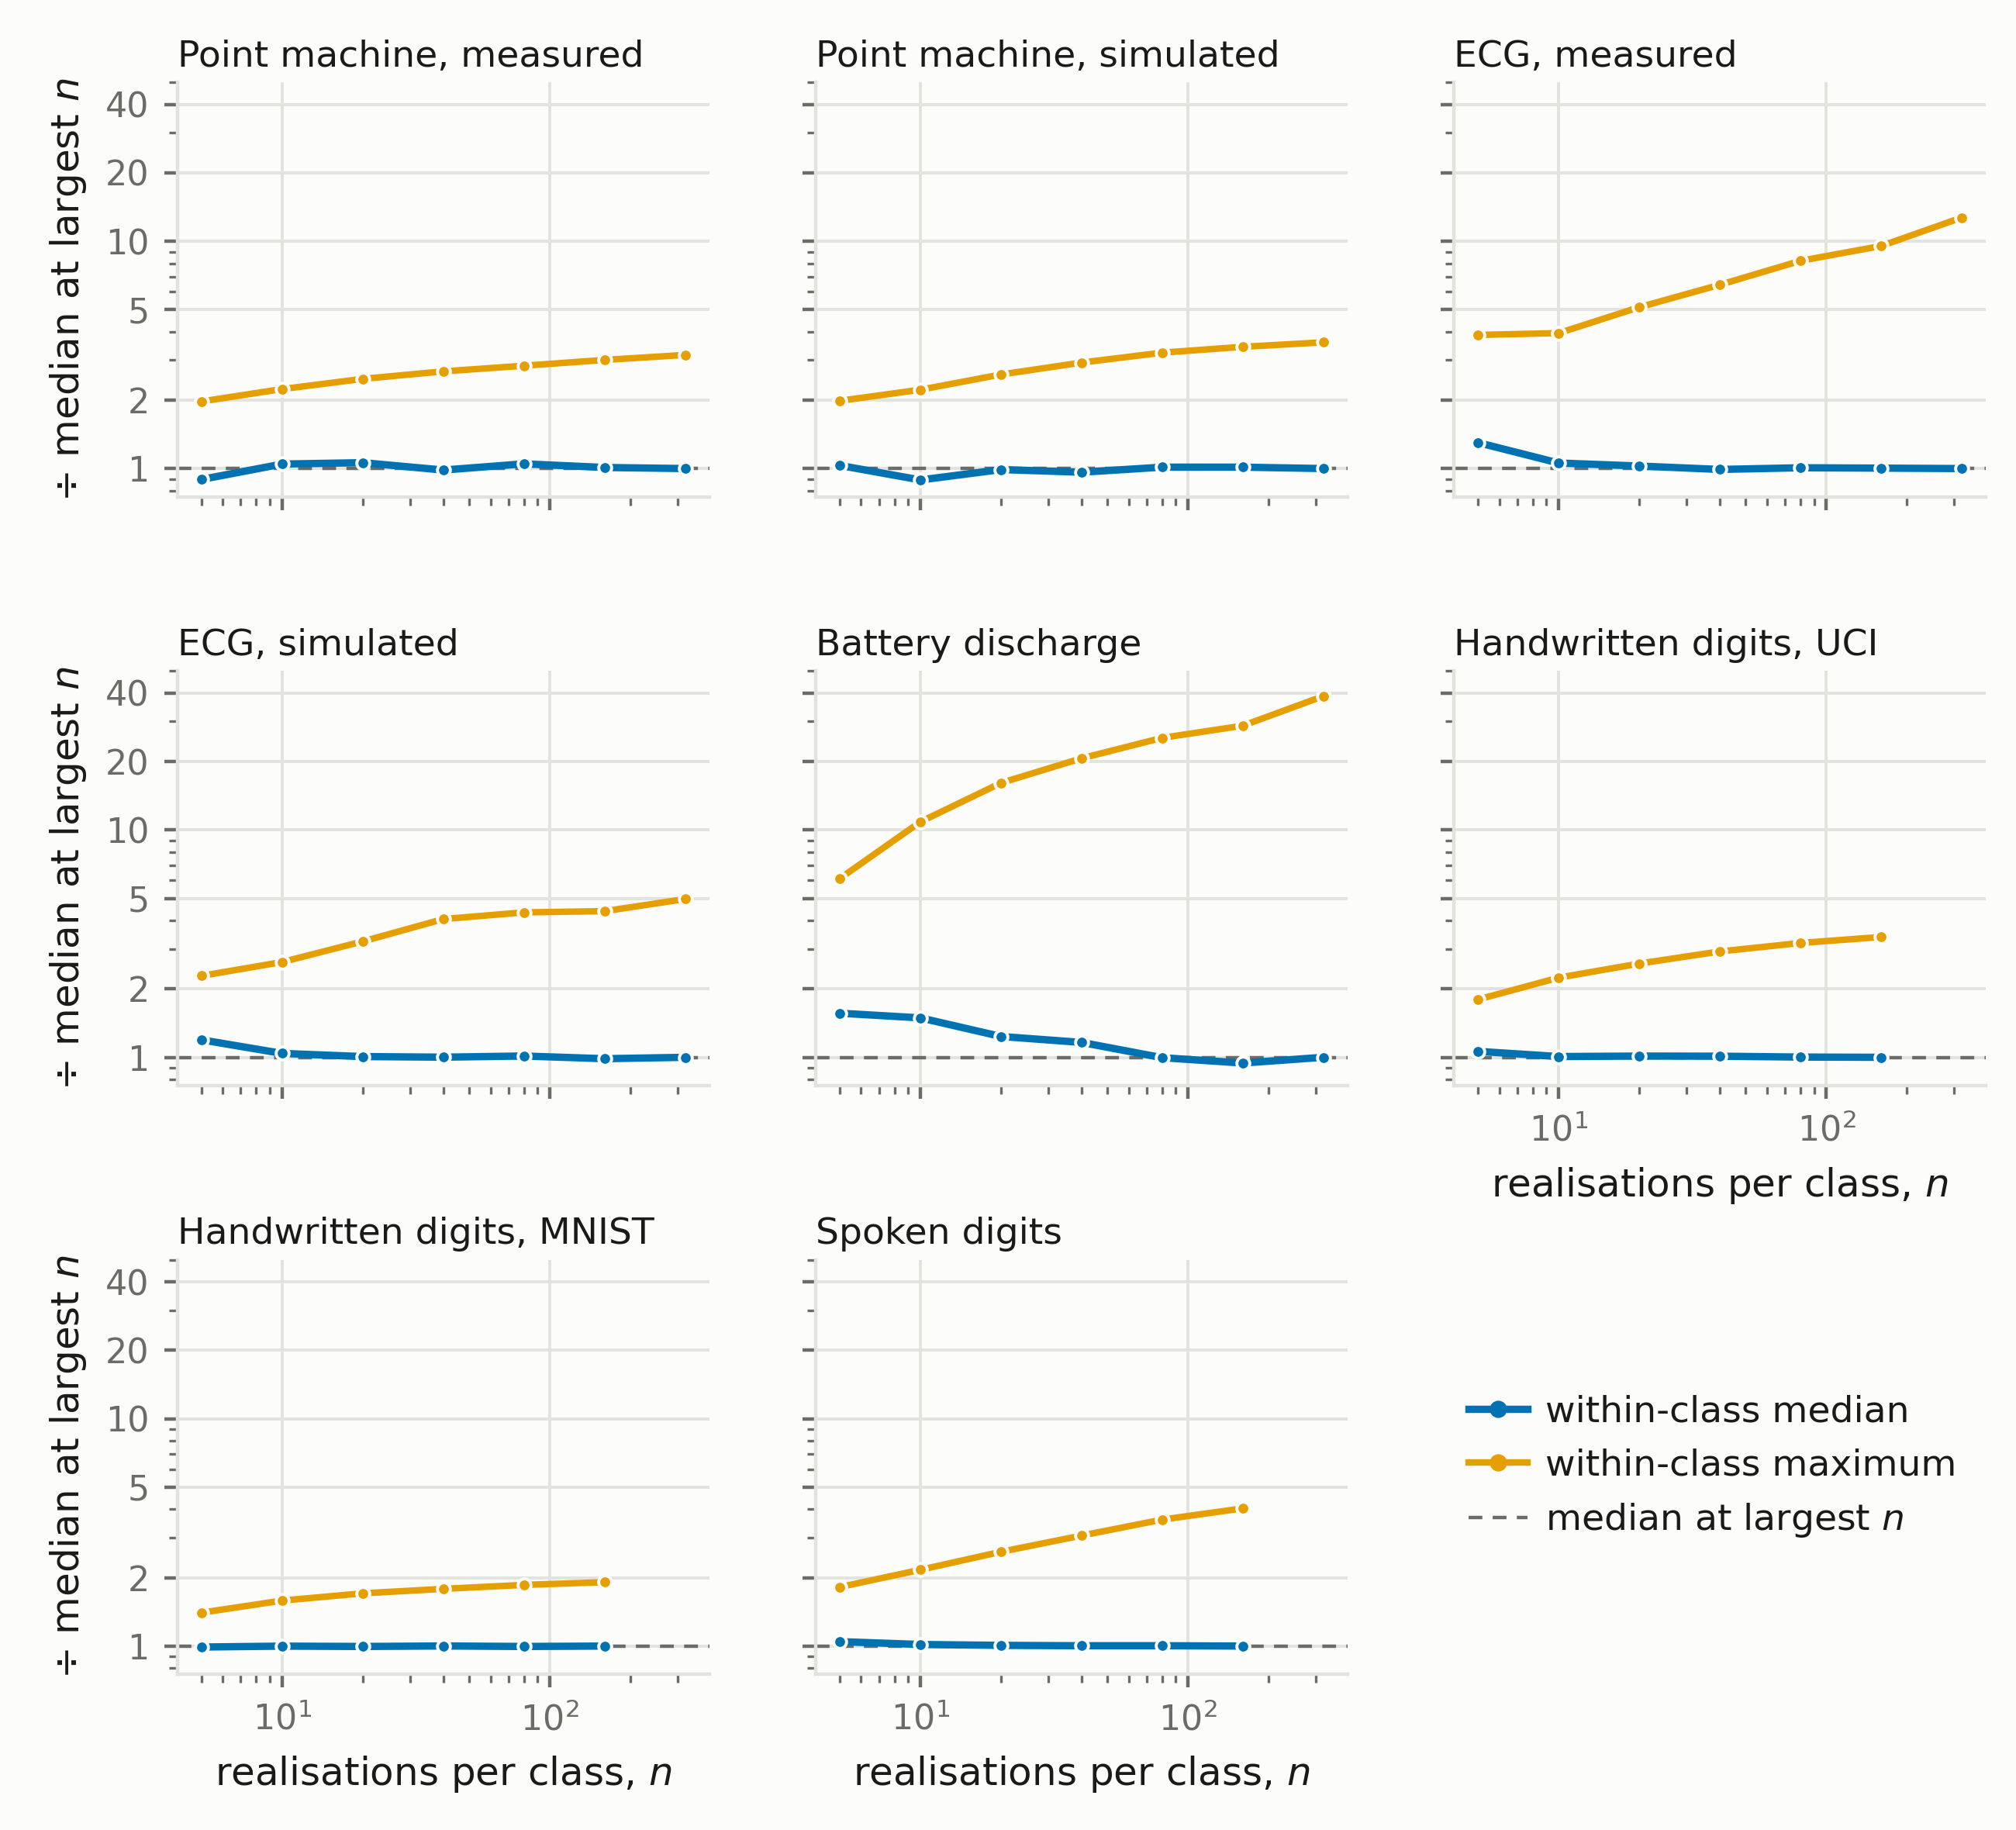
\includegraphics[width=\textwidth]{fig_bulk_boundary.png}
\caption{\small Within each class, the median distance between realisations
(blue) and the maximum distance between them (orange), against the number of
realisations per class, each divided by that class's median at the largest
$n$. Both axes are logarithmic and shared across the eight panels, so what is
compared is the shape and not the units; the dashed line is that reference
value of one. Everything is cosine distance, the metric declared in
Section~\ref{sec:methods}. The median is flat in every panel; the maximum
climbs in every panel and does not level off. These replace six
per-domain saturation figures computed during initial stages of this work,
which set their vertical scale from a comparison of a sample with itself at the
smallest $n$ and mixed a euclidean radius with a cosine Hausdorff distance
inside one panel.}
\label{fig:bulk_boundary}
\end{figure}

\section{Digit Datasets: Structural Consistency Across Representations}
\label{sec:results-digits}

The physical domains above are single concepts measured against themselves. The
digit sets are the other case: ten concepts that must also be told apart. They
are included for three reasons. They provide a conceptually transparent
illustration of the framework, as the underlying invariant class is intuitively
grasped. Furthermore, they admit a formally declared invariance group, thereby
satisfying the scope condition delineated in Section~\ref{sec:scope}: a
handwritten digit constitutes a single symbol subject to geometric
transformations, forming an orbit rather than a loosely defined semantic
category. Finally, one dataset comprises acoustic time series rather than images,
which is where the account is most likely to break.

Three sets are used throughout: the $8\times8$ UCI optical
digits~\citep{uci_optdigits}, MNIST at $28\times28$~\citep{lecun1998mnist}, and
the Free Spoken Digit Dataset~\citep{fsdd} as log-mel spectrograms. Each
class is a concept, each realisation is a point, and nothing is trained. The
declared group is deskew for the two image sets --- one operation, applied or
not, reported both ways --- and, for the spoken set, the speaker and the rate,
as discussed in Section~\ref{sec:spoken-duration}.

\subsection{Alignment of the Covering Number with the Underlying Concept}

The convergence curve this section rests on is reported per set in
Table~\ref{tab:saturation_summary}, averaged over each set's ten concepts.
Appendix~\ref{app:digits-per-class} details the thirty concepts individually,
ensuring that class averaging does not mask underlying heterogeneity. The
analysis confirms structural consistency: while the absolute covering limits
within a single dataset may vary by a factor of up to $2.27$, the empirical
radius stabilises after approximately a dozen encounters across all thirty
classes.


Table~\ref{tab:gate} contrasts each real class with an \emph{arbitrary} class
of the same size, drawn at random from the pool of all ten digits, at five
resolutions taken from the within-class distance percentiles of the data
itself. By definition, both sets admit finite covering numbers due to their
uniform boundedness. The distinguishing metric is the cardinality of the cover.
An intrinsic class requires between $1.3$ and $3.8$ times fewer exemplars to
cover than a random ensemble of identical size at the same resolution. This
ratio strictly exceeds unity across all resolutions and datasets.

The covering numbers themselves are small. At the median within-class
resolution a UCI class needs $9.6$ exemplars, an MNIST class $19.8$, and a
spoken class $6.7$ --- against $36.1$, $50.6$ and $12.2$ for arbitrary classes
of the same size. This is the same order as the four to twenty-one
exemplars required to cover the continuous physical processes analysed
previously, despite the fundamental differences in their generating mechanisms.

\begin{table}[!htbp]\centering\small
\fitwidth{\begin{tabular}{llrrrrr}
\toprule
dataset & quantity & \multicolumn{5}{c}{$\varepsilon$ (within-class percentile)} \\
& & p5 & p25 & p50 & p75 & p90 \\
\midrule
UCI digits 8x8 & $\varepsilon$ & 0.054 & 0.105 & 0.162 & 0.237 & 0.316 \\
 & $|S|$ real & 69.8 & 22.2 & 9.6 & 4.4 & 2.4 \\
 & $|S|$ arbitrary & 134.6 & 71.9 & 36.1 & 15.9 & 7.3 \\
 & ratio & \textbf{1.93} & \textbf{3.24} & \textbf{3.75} & \textbf{3.66} & \textbf{3.09} \\
\midrule
MNIST 28x28 & $\varepsilon$ & 0.219 & 0.362 & 0.471 & 0.581 & 0.678 \\
 & $|S|$ real & 206.3 & 53.0 & 19.8 & 8.2 & 3.9 \\
 & $|S|$ arbitrary & 362.2 & 129.4 & 50.6 & 18.4 & 7.9 \\
 & ratio & \textbf{1.76} & \textbf{2.44} & \textbf{2.55} & \textbf{2.25} & \textbf{2.03} \\
\midrule
Spoken digits (FSDD) & $\varepsilon$ & 0.010 & 0.028 & 0.040 & 0.054 & 0.069 \\
 & $|S|$ real & 80.2 & 13.4 & 6.7 & 4.1 & 2.9 \\
 & $|S|$ arbitrary & 185.0 & 34.1 & 12.2 & 6.0 & 3.6 \\
 & ratio & \textbf{2.31} & \textbf{2.55} & \textbf{1.80} & \textbf{1.48} & \textbf{1.27} \\
\bottomrule
\end{tabular}
}
\caption{\small The gate. $|S(\varepsilon)|$ for a real class and for an
arbitrary class of the same size, averaged over the ten classes and five
arrival orders, at five resolutions read off the within-class distance
distribution. The ratio is the signal: a concept is cheaper to cover than a
bag of the same size.}
\label{tab:gate}
\end{table}

\subsection{Separability is a property of the representation}

While this covering ratio confirms that the $\varepsilon$-net successfully
distinguishes an intrinsic concept from unstructured data, it does not directly
quantify inter-class separability. If all ten classes share a dominant structural
component, a random ensemble will come out nearly as narrow as one class, driving the ratio toward unity without reflecting true class
overlap. A robust measure of separability must evaluate the distance between each
class and the union of the remaining nine classes.

Table~\ref{tab:separability} reports it as
$P(d_{\mathrm{within}} < d_{\mathrm{between}})$, where $1/2$ is chance. Two
readings matter. First, the three sets differ, and the differences are large:
$0.87$ for UCI, $0.75$ for MNIST, $0.63$ for the spoken set. Spoken digits are
genuinely harder to separate under their declared observable than written ones,
and the duration quotient of Section~\ref{sec:spoken-duration} narrows that gap
without closing it --- with the zero padding the same quantity is $0.55$, which
is very nearly chance.

Second, and more to this paper's subject: \emph{the number does not move with
$n$}. From five realisations per class to a hundred and sixty --- thirty-two
times the evidence --- separability changes by less than one part in a hundred
in every row. This is what one should expect of a property of the
representation rather than of an estimator that improves, and it is worth
stating in the direction that is useful: five realisations per class are
already enough to know how separable one's classes are. That is a statement
about the cost of \emph{estimating} separability. It is not a claim that more
data cannot help a trained classifier, which is a question about a different
object.

\begin{table}[!htbp]\centering\small
\fitwidth{\begin{tabular}{lrrrrrrrr}
\toprule
& \multicolumn{6}{c}{separability at $n$ per class} & within & between \\
\cmidrule(lr){2-7}
dataset & 5 & 10 & 20 & 40 & 80 & 160 & median & median \\
\midrule
UCI digits 8x8 & 0.874 & 0.870 & 0.868 & 0.861 & 0.865 & 0.866 & 0.166 & 0.323 \\
MNIST 28x28 & 0.772 & 0.760 & 0.760 & 0.752 & 0.755 & 0.752 & 0.474 & 0.616 \\
Spoken digits, zero-padded & 0.546 & 0.559 & 0.555 & 0.552 & 0.554 & 0.555 & 0.025 & 0.028 \\
Spoken digits (FSDD) & 0.622 & 0.635 & 0.631 & 0.629 & 0.628 & 0.630 & 0.041 & 0.049 \\
\bottomrule
\end{tabular}
% separability = P(d_within < d_between), mean over the ten
%   classes; 0.5 is chance. Each class against the other nine.
% The medians are at the largest n.
}
\caption{\small Each class against the other nine.
$P(d_{\mathrm{within}} < d_{\mathrm{between}})$, mean over the ten classes,
against the number of realisations per class; $0.5$ is chance. The spoken set
is shown under both observables. The last two columns are the within- and
between-class median distances at the largest $n$: for the zero-padded spoken
set they are $0.025$ and $0.028$, which is the collapse in one line.}
\label{tab:separability}
\end{table}

\subsection{The decision rule}

Where this paper classifies, the rule is the following. Keep $k$ exemplars per
class; given a new realisation, measure its distance to each class's exemplars
and take the smallest. That is nearest-neighbour classification with per-class
prototypes~\citep{cover1967nearest}. It is not new, it is not proposed here as a
method, and presenting it as one would be worse than useless. It appears
because it is the simplest rule that consumes exactly what the geometry
supplies --- a set of remembered exemplars and a distance --- so that what is
being measured is the geometry and not an architecture.

Two things about it are ours, and neither is the rule.

\paragraph{The geometry sets the budget, not the choice.}
The table below compares two ways of spending the same budget of $k$ exemplars
per class. \emph{Any $k$} means the $k$ are drawn from the class without being
chosen --- it is not a selection method, and naming it that way would miss the
point, which is that no selection is performed. \emph{The net's $k$} means the
first $k$ points of the greedy $\varepsilon$-net. The net is an instrument for
measuring a set, and it is tempting to promote it to a selection rule: if a net
of size $k$ covers the class, keep those $k$. We tried it, and
Table~\ref{tab:selector} reports that it loses. The net's \emph{first} point is an excellent single prototype
--- it is the point nearest the centre, and at $k=1$ it beats a random draw by
a wide margin in all three sets, $0.87$ against $0.62$ on UCI and $0.69$
against $0.43$ on MNIST. Its subsequent points are the worst possible
additions. A greedy net walks to the extremes of a set, because that is what
covering means; a nearest-neighbour rule wants the bulk, because that is where
the mass is. So the net's curve flattens while the unselected one keeps
climbing, and on MNIST at twenty exemplars per class --- roughly the covering
number at the median resolution --- unselected exemplars reach $0.807$ and the
net's $0.714$.

We report this because it is the honest reading of what the measurement
licenses, and because the honest reading is the stronger claim. ``$k$ exemplars
suffice, whichever they are'' says the structure is in the class. ``The right
$k$ suffice'' would say it is in a clever selection.

\begin{table}[!htbp]\centering\small
\fitwidth{\begin{tabular}{llrrrrrrrrr}
\toprule
& & \multicolumn{9}{c}{prototypes per class} \\
\cmidrule(lr){3-11}
dataset & exemplars & 1 & 2 & 3 & 5 & 8 & 12 & 20 & 32 & 50 \\
\midrule
UCI digits 8x8 & any $k$ & 0.622 & 0.751 & 0.805 & 0.868 & 0.903 & 0.929 & 0.954 & 0.969 & 0.978 \\
UCI digits 8x8 & the net's $k$ & 0.867 & 0.875 & 0.880 & 0.901 & 0.924 & 0.944 & 0.958 & 0.971 & 0.980 \\
\midrule
MNIST 28x28 & any $k$ & 0.425 & 0.539 & 0.588 & 0.665 & 0.726 & 0.772 & 0.807 & 0.836 & 0.869 \\
MNIST 28x28 & the net's $k$ & 0.692 & 0.694 & 0.685 & 0.691 & 0.699 & 0.714 & 0.714 & 0.720 & 0.726 \\
\midrule
Spoken digits (FSDD) & any $k$ & 0.240 & 0.348 & 0.424 & 0.515 & 0.599 & 0.686 & 0.797 & 0.866 & 0.896 \\
Spoken digits (FSDD) & the net's $k$ & 0.401 & 0.410 & 0.397 & 0.438 & 0.531 & 0.642 & 0.780 & 0.867 & 0.914 \\
\bottomrule
\end{tabular}
% 1-NN over ten per-class exemplar sets, same split and seeds.
% "any k" = drawn without selection; "the net's k" = the greedy net's
%   first k points. The names carry the claim: the point is that the k
%   need not be chosen, not that random is a method.
% The net walks to the extremes; the rule wants the bulk.
}
\caption{\small Exemplars drawn without selection against exemplars chosen by
the greedy net, at equal budget $k$. Same split, same seeds, same 1-NN decision
over the ten exemplar sets; accuracy on held-out realisations, mean of ten
draws. \emph{Any $k$} is not a selection method: the column exists to show that
none is needed. The net's first point is the best single exemplar in every set;
its later points buy coverage rather than mass.}
\label{tab:selector}
\end{table}

\paragraph{The operating point is requested, not discovered.}
The rule has one parameter, the tolerance $\tau$, and it belongs to the
observer rather than to the phenomenon: it is set, not fitted. Raising it can
only admit more, so it trades precision against recall monotonically, and the
memory the rule needs at that setting is exactly $|S(\tau)|$. A question no
trained classifier answers in advance therefore has an answer here: how much
must be stored to reach a demanded $F_1$. Table~\ref{tab:operating} answers it,
and reports where the demand exceeds what this rule can do at all: the ceiling
is $0.906$ for UCI raw, $0.811$ for the spoken set, $0.763$ for MNIST.

That ceiling is the rule's, not the phenomenon's. Lowering $\tau$ to keep more exemplars costs
recall faster than it buys precision, so no additional memory reaches a target
above the ceiling; every one of the five curves peaks in the interior of the
$\tau$ grid rather than at its edge, which is how we know the maximum belongs
to the rule and not to where we stopped looking. But on the same data, the same
observable and the same exemplars, a rule that is allowed to \emph{compare}
does better: Table~\ref{tab:learning_target} reports a nearest-neighbour
readout reaching $95\%$ accuracy on UCI with twenty exemplars per class. The
distance between the two tables is what refusing to compare costs, and that is
the reason to print both.

That MNIST is the hardest row here, and spoken not the easiest to separate but
the second easiest to \emph{accept}, is a reminder that these are two different
questions. A one-class rule must answer without comparing.
Table~\ref{tab:decision} separates them: how often the candidate set contains
exactly one class, several, or none; how accurate the answer is when it
contains one; and how much room a decision rule would have if it were allowed
to compare.

\begin{table}[!htbp]\centering\small
\fitwidth{\begin{tabular}{llrrrr}
\toprule
& & \multicolumn{3}{c}{exemplars per class required} & \\
\cmidrule(lr){3-5}
dataset & quotient & $F_1\!\ge\!0.80$ & $F_1\!\ge\!0.90$ & $F_1\!\ge\!0.95$ & ceiling $F_1$ \\
\midrule
UCI digits 8x8 & raw & 13 & 23 & --- & $0.906 \pm 0.006$ \\
UCI digits 8x8 & quotient (deskew) & 14 & --- & --- & $0.881 \pm 0.005$ \\
MNIST 28x28 & raw & --- & --- & --- & $0.763 \pm 0.007$ \\
MNIST 28x28 & quotient (deskew) & --- & --- & --- & $0.768 \pm 0.006$ \\
Spoken digits (FSDD) & raw & 70 & --- & --- & $0.811 \pm 0.008$ \\
\bottomrule
\end{tabular}
% One-class rule, one-vs-rest, single global tau.
% '---' = the demanded F1 is above this rule's ceiling, given
%   in the last column. NOT a claim about the phenomenon: the
%   comparative readout of table_learning_target reaches
%   accuracies this rule cannot, on the same data.
% Every curve peaks inside the tau grid, so the ceiling is the
%   rule's and not the grid's.
}
\caption{\small Exemplars per class required to reach a demanded $F_1$ under
the one-class rule at a single global $\tau$, and the ceiling of that rule. A
dash means the demanded $F_1$ is above that ceiling, which is given in the last
column; it is a limit of a rule that must answer without comparing, at this
pool size, and not a limit of the phenomenon.}
\label{tab:operating}
\end{table}

\begin{table}[!htbp]\centering\small
\fitwidth{\begin{tabular}{llrrrrrr}
\toprule
& & \multicolumn{3}{c}{candidate set} & accuracy & set & forced \\
\cmidrule(lr){3-5}
dataset & quotient & one & several & none & on \emph{one} & coverage & choice \\
\midrule
UCI digits 8x8 & raw & 0.82 & 0.10 & 0.08 & 0.995 & 0.915 & 0.970 \\
UCI digits 8x8 & quotient (deskew) & 0.78 & 0.12 & 0.10 & 0.991 & 0.896 & 0.967 \\
MNIST 28x28 & raw & 0.61 & 0.17 & 0.21 & 0.979 & 0.771 & 0.920 \\
MNIST 28x28 & quotient (deskew) & 0.63 & 0.07 & 0.30 & 0.993 & 0.695 & 0.962 \\
Spoken digits (FSDD) & raw & 0.70 & 0.15 & 0.15 & 0.986 & 0.833 & 0.933 \\
\bottomrule
\end{tabular}
% At the tau maximising one-class F1. Set coverage is how often
% the true class is among the candidates; the gap between it and
% forced-choice accuracy is the room a decision rule has.
}
\caption{\small At the $\tau$ maximising one-class $F_1$. Set coverage is how
often the true class is among the candidates; the gap between it and
forced-choice accuracy is the room a decision rule has.}
\label{tab:decision}
\end{table}

\subsection{A declared invariance is sample efficiency}

The two image sets admit one declared operation, deskew, and it is applied or
not with everything else held fixed. Table~\ref{tab:learning_target} reports
how many realisations per class three unrelated readouts --- a linear SVM,
logistic regression, and 1-NN --- need to reach a common absolute accuracy
under each condition.

On MNIST at $0.85$ the raw condition needs $80$, $80$ and $40$ per class and
the quotiented condition $10$, $20$ and $20$: factors of eight, four and two.
At $0.90$ the raw condition needs $1280$, $1280$ and $160$ against $40$, $80$
and $40$: factors of thirty-two, sixteen and four. The factor grows with the
accuracy demanded, which is what one expects if the quotient is removing
variation that has to be learned example by example otherwise.

Three methods that share nothing beyond consuming the same vectors move
together, which is the point: what is being hit is a property of the
representation and not of any one estimator.

\begin{table}[!htbp]\centering\small
\fitwidth{\begin{tabular}{l l r r r r r r r r r}
\toprule
& & \multicolumn{3}{c}{linear SVM} & \multicolumn{3}{c}{logistic} & \multicolumn{3}{c}{1-NN} \\
\cmidrule(lr){3-5}\cmidrule(lr){6-8}\cmidrule(lr){9-11}
dataset & quotient & 0.85 & 0.90 & 0.95 & 0.85 & 0.90 & 0.95 & 0.85 & 0.90 & 0.95 \\
\midrule
UCI digits 8x8 & raw & 10 & 20 & 80 & 10 & 40 & --- & 5 & 10 & 20 \\
UCI digits 8x8 & quotient (deskew) & 10 & 20 & 80 & 10 & 40 & --- & 10 & 10 & 20 \\
MNIST 28x28 & raw & 80 & 1280 & --- & 80 & 1280 & --- & 40 & 160 & 1280 \\
MNIST 28x28 & quotient (deskew) & 10 & 40 & --- & 20 & 80 & --- & 20 & 40 & 160 \\
Spoken digits (FSDD) & raw & 80 & 160 & --- & --- & --- & --- & 40 & 80 & 160 \\
\bottomrule
\end{tabular}
% samples per class needed to reach a COMMON absolute accuracy.
% Comparable across quotients; the knee table is not.
}
\caption{\small Realisations per class needed to reach a common absolute
accuracy. Comparable across quotients, which the knee table
(Table~\ref{tab:learning}) is not. The spoken set has no deskew row: deskew
acts on image axes and a log-mel spectrogram has none.}
\label{tab:learning_target}
\end{table}

\begin{table}[!htbp]\centering\small
\fitwidth{\begin{tabular}{llrrrr}
\toprule
& & \multicolumn{3}{c}{accuracy knee: smallest $n$ per class reaching 95\% of its own maximum} & within-class \\
\cmidrule(lr){3-5}
dataset & quotient & linear SVM & logistic & 1-NN & median drift \\
\midrule
UCI digits 8x8 & raw & 20 & 20 & 20 & 10\% \\
UCI digits 8x8 & quotient (deskew) & 20 & 20 & 20 & 14\% \\
MNIST 28x28 & raw & 160 & 160 & 320 & 0\% \\
MNIST 28x28 & quotient (deskew) & 40 & 80 & 160 & 7\% \\
Spoken digits (FSDD) & raw & 80 & 160 & 80 & 10\% \\
\bottomrule
\end{tabular}
}
\caption{\small The accuracy knee --- the smallest $n$ per class reaching
$95\%$ of that classifier's own maximum --- and the drift of the within-class
median from the first grid point. The knee is a per-condition quantity and is
not comparable across quotients.}
\label{tab:learning}
\end{table}

\subsection{Controls}

Table~\ref{tab:controls} separates the declared operation from two things it
might be confused with. \textsc{blur} resamples without aligning, \textsc{deskew}
resamples and aligns, and \textsc{randshear} resamples and destroys the
alignment. If the gain came from resampling, blur would show it; if it came
from the alignment, deskew alone would, and randshear would remove it. The
latter is what happens.

Table~\ref{tab:dimension} reports intrinsic dimension under the declared
protocol of Section~\ref{sec:methods}, with its calibration against spheres of
known dimension at matched $n$ printed beside it, so the number is read next to
the evidence for how far it can be trusted. Both digit sets sit above the
calibrated range and their values should be read as ordinal. The ordering they
give is the same one every other measurement here gives: a real class is lower
dimensional than an arbitrary class of the same size, by a factor of $1.2$ to
$1.5$.

\begin{table}[!htbp]\centering\small
\fitwidth{\begin{tabular}{lccc}
\toprule
condition & resampling & alignment & $P(d_{\mathrm{within}} < d_{\mathrm{between}})$ \\
\midrule
\textsc{randshear} & yes & destroyed & 0.715 \\
raw & no & --- & 0.754 \\
\textsc{blur} & yes & none & 0.767 \\
\textsc{deskew} & yes & applied & \textbf{0.838} \\
\bottomrule
\end{tabular}
}
\caption{\small Resampling against alignment on MNIST.
$P(d_{\mathrm{within}} < d_{\mathrm{between}})$ at $n=640$.}
\label{tab:controls}
\end{table}

\begin{table}[!htbp]\centering\small
\fitwidth{\begin{tabular}{lrrrl}
\toprule
set & $n$ & pts & $\hat{d}$ & \\
\midrule
PM real (nominal) & 600 & 9 & $2.47 \pm 0.15$ &  \\
PM simulated & 600 & 9 & $2.54 \pm 0.12$ &  \\
ECG real (MIT-BIH) & 600 & 9 & $2.28 \pm 0.07$ &  \\
ECG simulated & 600 & 9 & $3.82 \pm 0.05$ &  \\
Battery real (NASA) & 600 & 8 & $1.89 \pm 0.07$ &  \\
\midrule
UCI digits 8x8, real classes & 174 & --- & $3.87$ & above calibrated range \\
UCI digits 8x8, arbitrary class & 174 & --- & $4.68$ & control \\
MNIST 28x28, real classes & 600 & --- & $6.62$ & above calibrated range \\
MNIST 28x28, arbitrary class & 600 & --- & $8.52$ & control \\
Spoken digits (FSDD), real classes & 300 & --- & $3.49$ & above calibrated range \\
Spoken digits (FSDD), arbitrary class & 300 & --- & $5.12$ & control \\
\midrule
\multicolumn{5}{l}{\emph{calibration: same protocol on $S^d$, $d$ known}} \\
$n=174$ & & & $d{=}1\!\to\!0.90$, $d{=}2\!\to\!1.63$, $d{=}3\!\to\!2.37$, $d{=}4\!\to\!2.78$, $d{=}5\!\to\!3.31$, $d{=}6\!\to\!3.72$ & \\
$n=300$ & & & $d{=}1\!\to\!0.93$, $d{=}2\!\to\!1.74$, $d{=}3\!\to\!2.44$, $d{=}4\!\to\!2.90$, $d{=}5\!\to\!3.43$, $d{=}6\!\to\!4.05$ & \\
$n=600$ & & & $d{=}1\!\to\!0.97$, $d{=}2\!\to\!1.81$, $d{=}3\!\to\!2.49$, $d{=}4\!\to\!3.10$, $d{=}5\!\to\!3.65$, $d{=}6\!\to\!4.12$ & \\
\bottomrule
\end{tabular}
}
\caption{\small Intrinsic dimension under the declared protocol, with the
calibration that bounds its interpretation.}
\label{tab:dimension}
\end{table}


% -------------------------------
% 7. Discussion
% -------------------------------
\section{Discussion}
\label{sec:discussion}

\subsection{What this work establishes}

This work establishes two magnitudes, and they are magnitudes rather than
properties. In electromechanical railway point
machines, electrochemical battery discharge trajectories, physiological ECG
waveforms, solar irradiance profiles, tidal cycles, handwritten digits and
spoken digits --- seven phenomena, together with deterministic simulators of
two of them --- an observer's estimate of a class's size settles \emph{fast}:
ten or twelve realisations in every one of ten convergence curves. And in the
five domains where the surrogate control was run, the regions are \emph{small}:
four to twenty-one exemplars cover a class at its own resolution, against a
surrogate carrying the same spectrum and amplitude distribution that needs the
whole pool. The control does not report the same verdict everywhere, and that is
part of the result --- in the tidal domain the same surrogate needs almost as
little as the real signal, and it was not run on the digit sets at all.

Neither magnitude follows from compactness. That these sets are compact is
forced by Arzel\`a--Ascoli once H1 and H2 are granted, and
Section~\ref{sec:hypotheses} says so before any measurement is reported. The
same asymmetry is visible in the classical theory: metric entropy is computed
or bounded for function classes chosen for their analytic tractability
\citep{kolmogorov1993entropy, dudley1967sizes}, and in learning theory the
covering number enters as a bound on a hypothesis class rather than as a
measurement of data \citep{cucker2001mathematical, zhou2002covering}. What
the theoretical section contributes is the bookkeeping around it --- the
statement in the Banach space $C^0([0,T])$, a Monte Carlo estimator for the
perceptual radius, and conditions under which that estimator converges as
sampling becomes dense in the state--condition space. How large the sets are,
and how quickly an observer can know, the analysis leaves entirely open.

The separation that organises all of it is between the bulk of a class and its
boundary. The interior is a functional of the measure and is fixed after a
handful of encounters. The boundary is a functional of the support, and support
functionals are known to be the hard ones to estimate from finite samples
\citep{devroye1980detection, scholkopf2001estimating}; it is still growing at
every sample size we can reach:
Section~\ref{sec:bulk-boundary} measures a within-class maximum at
thirty-nine times its own median in the battery domain and rising. Every
convergence result in this paper is about the first quantity.

\subsection{Self-supervised emergence of perceptual structure}

A central implication of the framework is that perceptual structure can
emerge in a self-supervised manner when explicit physical equations are
unavailable. The perceptual manifold $\mathcal{M}$ and its radius $r$ need
not be specified a priori: they are discovered progressively from the
stream of observations by tracking the evolution of the empirical radius
$\hat r_n$. When $\hat r_n$ enters and stays inside a stated band around its
limit, the observer has a bound on how much the estimate can still move.

In this sense, deterministic physical systems support a form of self-supervised
learning: by repeatedly observing the same process under varying conditions, an
agent can establish \emph{how large} the corresponding perceptual class is, and
how much more observation could still change that estimate, without labels,
external supervision or a parametric model. The self-supervised literature
obtains representations without labels by contrasting or matching augmented
views of the same datum \citep{chen2020simple, caron2021emerging,
balestriero2023cookbook}; the augmentations there play the role our declared
quotient plays here, and the difference is that they are used to \emph{train} a
representation whereas we use the declared group to \emph{measure} a set. No
representation is fitted anywhere in this paper. What it cannot establish this way
is where the class ends. The two are different quantities and only the first
converges (Section~\ref{sec:bulk-boundary}); an agent that waited to know the
boundary would wait indefinitely, and one that needs to act on the bulk can act
after a dozen encounters. The five physical domains and the three digit sets of
Section~\ref{sec:results-digits} agree on that schedule, in two modalities and
across ten concepts that must also be told apart.

\subsection{Algorithmic and industrial implications}

The compact-manifold viewpoint offers practical advantages for sensing,
diagnosis and similarity search. In domains such as railway maintenance,
battery monitoring and physiological signal analysis, the class provides a
reference model against which new observations can be compared, and deviations
can be quantified as distances to it. That framing is the standard one in
anomaly detection, where a model of normality is built and departures from it
are scored \citep{chandola2009anomaly, scholkopf2001estimating}; what is missing
from it, and what the measurements here supply, is the size of the nominal
dataset the model of normality requires. Because the estimate of the radius
settles after a modest number of samples, such a reference can be built from a
small dataset and refined incrementally.

A critical consequence of this framework is its operational utility for
industrial commissioning. Establishing a reference model for a new installation
requires specifying the requisite nominal data volume, a decision conventionally
based on heuristics. This framework formalises that decision as a bounded
calculation with a declared tolerance: achieving an estimate within ten per cent
of the limit requires approximately ten to twelve realisations across
all measured domains. Tighter tolerances (e.g., five per cent) introduce
domain-specific dependencies (ranging from 25 to 160 samples), while at one per cent, four of the ten curves never get there at all
(Section~\ref{sec:crossings}). A budget stated with its tolerance is a different
object from a rule of thumb, and it is the practical content of this work.

Early settling also bears on algorithm design. Once an observer's estimate has
stopped moving, additional realisations rarely change it, which suggests that
exhaustive comparison against a growing reference set can be replaced by
targeted refinement and early stopping. We note the direction without
instantiating it: the measurements here say what a budget is, not how to spend
it, and an algorithm built on early stopping would need its own evaluation
against the alternatives, which this paper does not attempt.

\subsection{Connections to world models and structured representations}

The geometric interpretation aligns with views in machine learning that
emphasise structured representations and world models
\citep{ha2018world, lecun2022path, bengio2013representation}. A deterministic
physical process implicitly defines a generative mechanism with stable
functional structure, operational invariants and bounded variability; the associated
perceptual class serves as a low-dimensional reference for the observations
such a mechanism admits. We say \emph{reference} and not \emph{complete
description}: the set of admissible observations is not something this
construction enumerates, and the extremes of it are exactly what does not
settle.

Unlike traditional latent-variable approaches, this framework does not rely on
probabilistic assumptions or explicit parameterisations. The class is defined
by the system itself, and the observer's task is to approximate its structure
using geometric measurements. This provides a deterministic counterpart to
world-model learning and suggests a way to combine physical constraints with
learned representations where governing equations are partially known.

The framework is complementary to JEPA-based architectures
\citep{lecun2022path, assran2023self} and to their vision--language
instantiations such as VL-JEPA~\citep{chen2025vljepa}. That line shows
empirically that predicting target embeddings in a continuous latent space
supports efficient learning; our results speak to why such an approach is
plausible in domains where H1, H2 and H3 hold, since the families of
realisations there occupy small regions on which continuous functionals are
universally approximable. The same reading applies to the sample-complexity
gains reported for invariant and equivariant models
\citep{anselmi2016unsupervised, elesedy2021provably, tahmasebi2023exact}: those
results price an invariance in the units of a learner's generalisation bound,
and the measurements here suggest what is being bought --- a smaller set to
cover, in a quantity that can be read off the phenomenon before a learner
exists. The qualification carried by H3 represents a critical boundary condition for such
learning guarantees. The universal approximation theorem established in
Section~\ref{sec:uat-section} needs only H1 and H2: the discretisation is our own grid, and equicontinuity settles what it costs. Hypothesis H3, in contrast,
dictates the physical well-posedness of the task: it determines whether the
desired target function can be mathematically formulated as a functional on the
observed signals at all. Using manifold-level quantities such
as the empirical radius and its settling schedule to analyse or regularise learned embedding spaces is a direction we
have not pursued.

\section{Conclusion}
\label{sec:conclusion}

This work establishes a deterministic functional--topological framework for perception, modelling the realisations of a physical process as a compact manifold in $C^0([0,T])$. Within this framework, identification reduces to distance minimisation and learning to the universal approximation of continuous functionals on compact domains. Empirical evaluation across seven phenomena---ranging from electromechanical and physiological signals to spoken digits---demonstrates that an observer's estimate of the class radius settles within ten per cent of its limit after merely ten to twelve encounters. This confirms that admissible signals in these domains occupy strictly bounded regions of functional space under the chosen representation, and that the size of these regions can be measured rapidly from sparse data without access to the underlying governing equations.

Consequently, perceptual structure can emerge in a self-supervised manner. While the true admissible set never ceases to expand---as extremal realisations continuously arrive---the observer's operational estimate stabilises early enough to be useful. This early saturation provides a principled geometric foundation for self-supervised learning, suggesting that similarity-search procedures and observers can operate efficiently on compact reference manifolds rather than unconstrained sequence spaces. Ultimately, this work offers a systematic account of how the deterministic structure imposed by the physical world shapes the representations that intelligent systems learn.

\section{Limitations and Future Work}
\label{sec:limitations}

The framework is intentionally focused on deterministic, continuous physical
processes whose benign variation forms a declarable group, and its scope is
correspondingly limited. Seven limitations are worth stating plainly: the first
two are about the conditions the account requires, the next three about the
instrument, and the last two about what the results do and do not license.

\paragraph{The hypotheses may fail, and the framework says how.}
We assume the underlying dynamics are effectively deterministic with bounded
noise, so that the set of realisations is uniformly bounded and equicontinuous.
Strongly stochastic systems, non-stationary regimes and processes with abrupt
structural changes may violate this, and the guarantees do not hold there.
Section~\ref{sec:hypotheses-per-domain} states the assumption per domain and
names where it is weakest in our own data --- the equicontinuity claim for solar
irradiance is the loosest in this paper and is labelled as such. Extending the
framework to regime-switching or explicitly stochastic systems is open.

\paragraph{The class must be an orbit, not a category.}
This is the sharper limit and it is a condition rather than a difficulty.
Section~\ref{sec:scope} requires that the benign variation of a class form a
declarable group. Handwritten digits and spoken digits satisfy it; photographs
of objects do not, because occlusion and background composition are not group
actions and there is nothing to quotient by. The framework does not extend to
semantic categories by measuring harder, and we do not claim it as future work.

\paragraph{What we decline to explain.}
Compactness is analytically assumed via physical constraints rather than derived, and the size of a class is empirically measured rather than predicted from first principles. A comprehensive geometric theory must eventually predict these parameters directly from system dynamics.

\paragraph{The theory and the measurement do not use the same metric.}
The theoretical results are stated in $C^0([0,T])$ with the supremum norm and
the induced Hausdorff distance, which is what makes Arzel\`a--Ascoli and the
universal approximation results available. Every measurement reported here uses
cosine distance on a fixed-length resampled vector, declared in
Section~\ref{sec:methods}. The two are not the same topology, and nothing in
this paper establishes that a result proved in one transfers to the other; the
supremum norm carries the theory and the cosine metric carries the experiments,
and the join between them is an assumption we have not tested. A systematic
comparison of alternative metrics --- Sobolev norms, weighted norms,
task-dependent distances --- is beyond this work and would be the first thing
we would want a critic to attack.

\paragraph{Dimensionality of the observable.}
Our measurements use one-dimensional traces and, for all three digit sets,
two-dimensional arrays read as fixed-length vectors --- pixel grids for the two
written sets and a mel-band by frame array for the spoken one. We do not treat video,
spatio-temporal fields or event-based data, where the discretisation choices
that this paper makes once per domain would have to be made again and would
carry more weight.

\paragraph{Finite sampling, and which quantity it limits.}
Estimation from finite data has two consequences and they are not the same. The
mean radius converges, and its estimate can be bounded by the criterion of
Section~\ref{sec:crossings}. The maximum does not: a maximum over a growing
sample is non-decreasing by construction, and where the support has thin tails
there is no rate. Rare operating regimes and degraded modes are therefore
underrepresented in any finite sample, and no sampling strategy repairs this ---
it is a property of what is being estimated and not a deficiency of how much
data was collected. This is why the paper reports the bulk and declines to
report a bound on the support, and why an operating point built on the tail of
a nominal set should be treated as provisional however much nominal data exists.

\paragraph{Existence results, and what we did and did not measure.}
The universal approximation result is existential: it states that suitable
approximators exist on a compact domain, not that a given architecture or
training procedure will find them, and we provide no complexity bounds. We do
report measured sample efficiency --- how many exemplars per class three
readout rules need to reach stated accuracies, with and without a declared
invariance (Section~\ref{sec:results-digits}) --- but a measurement on three
digit sets is not a bound. Bridging geometric
existence results and concrete learning algorithms remains open.

\paragraph{The perceptual layer only.}
The study addresses the acquisition of classes of admissible realisations and
the definition of a perceptual radius. It does not address higher-level
cognition, hierarchical planning or decision-making, and it is not a theory of
how perception works --- it is a measurement of the structure perception is
presented with. Extending this to multi-layer world models and control
architectures is a direction we have not taken.



\section*{Statements and Declarations}
\textbf{Funding}: No funding was received for conducting this study.

\textbf{Competing interests}: The author has no competing interests to declare that are relevant to the content of this article.

\textbf{Data and Code Availability}: All code and data required to reproduce the results in this manuscript are available in the public repository associated with this article at \url{https://github.com/eduardodisanti/shamayam}.

\textbf{Use of AI Tools}: AI tools were used for copy editing and to assist with parts of the analysis code; all content, methods, and conclusions were designed, verified, and are the responsibility of the author.

\bibliographystyle{tmlr}
\bibliography{references}

\appendix

\appendix


\section{Mathematical Framework and Proofs}\label{app:math_framework}


\label{sec:uat-section}

A perceptual process corresponds to mapping an observed signal to a numerical 
score, compatibility measure, or classification output. We formalise this as a 
continuous functional
\[
\Phi : \mathcal{M} \to \mathbb{R}
\]
defined on the compact perceptual manifold $\mathcal{M}$.

\subsection{Continuity of perceptual functionals}

Deterministic physical processes induce continuous variation of observations with
respect to changes in state or conditions. Thus, perceptual mappings that depend 
on physical structure (e.g.\ peak timing, amplitude, plateau stability) are 
naturally continuous in the supremum norm.

\begin{proposition}[Uniform Continuity on the Perceptual Manifold]
\label{prop:uniform}
If $\Phi$ is continuous on $\overline{\mathcal{M}}$, which
Theorem~\ref{thm:compactness} makes compact, then $\Phi$ is uniformly
continuous on $\overline{\mathcal{M}}$, hence on $\mathcal{M}$.
\end{proposition}

\noindent Proof: Heine–Cantor; see \ref{app:proofs}.

\subsection{Sampling an equicontinuous family}
\label{sec:sampling-lemma}

Because empirical evaluation operates on sampled vectors rather than continuous
functions, it is necessary to bound the approximation error induced by
discretisation. Let $\tau(\cdot)$ be the modulus of equicontinuity guaranteed
by H2: for every $\eta>0$, there exists $\tau(\eta)>0$ such that
$|t-s| \le \tau(\eta) \implies |x(t)-x(s)| \le \eta$ for all $x \in \mathcal{M}$.
For a uniform temporal grid $t_1 < \cdots < t_N$ on $[0,T]$ with spacing
$h = T/(N-1)$, we define the sampling operator
$\pi_N(x) = (x(t_1),\dots,x(t_N)) \in \mathbb{R}^N$.

\begin{lemma}[Sampling resolves an equicontinuous family]
\label{lem:sampling}
If $h \le \tau(\eta)$, then for all $x,y \in \mathcal{M}$
\[
\|x-y\|_\infty \;\le\; \|\pi_N(x)-\pi_N(y)\|_\infty + 2\eta .
\]
In particular $\pi_N(x) = \pi_N(y)$ implies $\|x-y\|_\infty \le 2\eta$.
\end{lemma}

\noindent Proof: See \ref{app:proofs}; it is three applications of the
triangle inequality.

This lemma formally translates the intuition that a band-limited signal is determined by samples taken finely enough. Crucially, it establishes that while
the sampling operator $\pi_N$ is not strictly injective on $\mathcal{M}$, it is
injective \emph{up to a tolerance of $2\eta$}, uniformly across the family. This
bounded metric distortion is sufficient to establish universal approximation
without assuming strict injectivity.

\subsection{Universal approximation of perceptual mappings}

\begin{theorem}[Universal Approximation on the Perceptual Manifold]
\label{thm:uat}
Assume H1 and H2, and let $\Phi : \overline{\mathcal{M}} \to \mathbb{R}$ be
continuous. Then for every $\varepsilon > 0$ there are a sampling resolution
$N$ and a feedforward network $N_\varepsilon : \mathbb{R}^N \to \mathbb{R}$ with
\[
\sup_{x \in \mathcal{M}} |\Phi(x) - N_\varepsilon(\pi_N(x))| < \varepsilon .
\]
The resolution is the one Lemma~\ref{lem:sampling} names: any grid finer than
the equicontinuity modulus at the accuracy demanded.
\end{theorem}

\noindent Proof: See \ref{app:proofs}. It is the Universal Approximation
Theorem \citep{cybenko1989approximation, hornik1991approximation} on the
compact set $\overline{\pi_N(\mathcal{M})}$, reached without inverting
$\pi_N$.

This formulation resolves an analytical limitation present in earlier geometric
analyses, which assumed the existence of a well-defined inverse mapping
$\pi_N^{-1}$ on $\mathcal{M}$. Lemma~\ref{lem:sampling} demonstrates that such
an assumption is unnecessary; the uniform equicontinuity guaranteed by H2
ensures that the variation of $\Phi$ across the pre-images of $\pi_N$ is strictly
bounded by $\varepsilon$. The proof constructs the approximation over a finite
$\varepsilon$-net, entirely avoiding the need for an inverse.

We distinguish the roles of H2 and H3 in this context, as they
govern distinct mappings. H3 governs the physical sensor mapping (process $\to$
continuous signal), asserting that the chosen observable reliably separates
distinct physical states. In contrast, H2 governs the discretisation mapping
(continuous signal $\to$ $\mathbb{R}^N$). The theorem above is about the second. H3 instead determines the well-posedness of the perceptual
task: if the physical observable maps distinct process states to the same
continuous signal, the desired task cannot be formulated as a well-defined
functional on $\mathcal{M}$, rendering the approximation theorem mathematically
valid but practically inapplicable. Consequently, H3 remains an empirical
hypothesis about the physical world, evaluated domain-by-domain in
Section~\ref{sec:hypotheses-per-domain}.

Finally, we note two limitations of this result. First, empirical failure to
separate two realisations at a finite resolution does not imply that the
underlying physical observable is non-injective; it indicates only that the
required resolution has not been met. Second, Theorem~\ref{thm:uat} establishes
solely the \emph{existence} of a finite approximating network. It is an existence
proof regarding representational capacity, not a statement regarding optimisation
or learning dynamics.

% ============================================================
% 4. HAUSDORFF RADIUS AND KNOWLEDGE BOUNDARIES
% ============================================================

\subsection{Monte Carlo estimation of the radius}

Sampling the physical system under varied $(s,\theta)$ provides empirical 
approximations of the supremum.

\begin{theorem}[Consistency of Monte Carlo Radius Estimation]
\label{thm:mc}
Let $(s_i,\theta_i)$ be samples whose support is dense in $\mathcal{S}\times\Theta$.
Define the estimator
\[
\hat{r}_n = \max_{1\le i \le n} \|f(s_i,\theta_i) - x_0\|_\infty.
\]
Then $\hat{r}_n \to r$ almost surely as $n\to\infty$.
\end{theorem}

\noindent Proof: See \ref{app:proofs}.

It is important to specify the precise nature of this convergence.
Theorem~\ref{thm:mc} establishes asymptotic consistency ($\hat{r}_n \to r$) under
dense sampling. However, it does not provide a statistical test to certify that
the support of $\mathcal{M}$ has been exhaustively sampled. Because the maximum
over a growing sample is strictly non-decreasing, it approaches its supremum at
an unconstrained rate (as analysed in Section~\ref{sec:bulk-boundary}).
Consequently, empirical evaluations employ the more tractable stability criterion
defined in Section~\ref{sec:crossings}: recording the number of observations
required for the estimate to enter and remain within a specified tolerance band.

\subsection{Identification as distance minimisation}

Finally, classification or recognition reduces to computing the distance from an
observation to the perceptual manifold.

Recognition is then minimum-distance classification in a compact functional
space: $x$ is admitted when $d_H(\{x\},\mathcal{M}) < \varepsilon$, for a
tolerance $\varepsilon$ that belongs to the observer's resolution and not to the
phenomenon. This thresholding approach directly applies the standard definition
of the distance from a point to a set. The critical parameter is the tolerance
$\varepsilon$, which, as established in Section~\ref{sec:scope}, is exogenously
determined by the observer's required resolution rather than discovered as an
intrinsic property of the phenomenon.

% -------------------------------
% 4.4 Self-Supervised Emergence of the Perceptual Radius
% -------------------------------
\subsection{Self-Supervised Emergence of the Perceptual Radius}

The perceptual radius $r$ plays a central role in determining the boundary of 
knowledge for a deterministic physical process. When the governing equations 
of the system are known, $r$ can be computed directly from the functional 
model:
\[
r = \sup_{s,\theta} \| f(s,\theta) - x_0 \|_\infty.
\]
However, in many real-world domains—electrochemical, physiological, or 
mechanical—the physical equations are partially known, high-dimensional, or 
altogether unavailable. In such cases, the observer must infer the perceptual 
structure directly from the observed signals.

\begin{proposition}[Self-Supervised Radius Identification]
\label{prop:selfsupervised}
Let $(x_i)_{i=1}^n$ be a sequence of realisations sampled from the physical 
process, and define the empirical radius
\[
\hat{r}_n = \max_{1 \le i \le n} \| x_i - x_0 \|_\infty.
\]
If sampling becomes dense in the underlying state–condition space, then 
$\hat{r}_n \to r$ almost surely. 
Thus, even without knowledge of the governing equations, the perceptual radius 
is recovered purely from observation.
\end{proposition}

\noindent Proof: Follows directly from Theorem~\ref{thm:mc} and compactness of 
$\mathcal{M}$; see \ref{app:proofs}.

\begin{remark}[Self-Supervised Perception]
The convergence of $\hat{r}_n$ implies that the observer operates in a 
self-supervised regime: the perceptual manifold $\mathcal{M}$ and its radius 
are discovered directly from the stream of observations, without labels, 
external supervision, or prior knowledge of the dynamics. 
As observations accumulate, what settles as realisations accumulate is the estimate, not the set. While the bulk of the probability mass is
characterised after a small number of samples, rare extremal states continue
to emerge asymptotically, as quantified in Section~\ref{sec:bulk-boundary}.
\end{remark}

This self-supervised property is consistent across all evaluated physical
domains. For railway point machines, where parametric physical models are
available, theoretical bounds and empirical estimates align. For battery
discharge and ECG signals, where the underlying electro-chemical or physiological
equations are often intractable, the empirical radius converges robustly. This
allows the size of the admissible region to be measured
directly from observational data, bypassing the need for explicit physical
modelling.

% ============================================================
% 6. METHODS  (including datasets)
% ============================================================


\label{app:proofs}

This appendix provides complete proofs for the theorems and propositions stated
in Sections~\ref{sec:deterministic}--\ref{sec:radius-section}. All results are stated in the Banach space 
$C^0([0,T])$ equipped with the supremum norm $\|x\|_\infty$.

% ---------------------------------------------------------
% A.1 Proof of the relative-compactness theorem
% ---------------------------------------------------------
\subsection{Proof of Theorem~\ref{thm:compactness} (Compactness of Deterministic Signals)}

\begin{proof}
Let $\mathcal{F} = \{ f(s,\theta) : s\in\mathcal{S},\;\theta\in\Theta\}$ be the
family generating the perceptual set $\mathcal{M}$.  
By assumption:

1. The family is \emph{uniformly bounded}, meaning there exists $M>0$ such that  
   $\|f(s,\theta)\|_\infty \le M$ for all $(s,\theta)$.

2. The family is \emph{equicontinuous}, i.e.\ for every $\varepsilon>0$ there
   exists $\delta>0$ such that for all $t_1,t_2\in[0,T]$:
   \[
   |t_1 - t_2| < \delta
   \quad\Rightarrow\quad
   |f(s,\theta)(t_1) - f(s,\theta)(t_2)| < \varepsilon.
   \]

By the Arzel\`a--Ascoli Theorem
\citep{rudin1991functional, royden2010real, conway1990course}, any uniformly
bounded and equicontinuous family of functions has compact closure in
$C^0([0,T])$. Thus $\overline{\mathcal{M}}$ is compact, which is what relative
compactness means.

We do not conclude that $\mathcal{M}$ itself is compact: that would require
$\mathcal{M}$ closed, which is not among the hypotheses. What transfers to
$\mathcal{M}$ without any further assumption is total boundedness, since a
subset of a totally bounded set is totally bounded. Hence for every
$\varepsilon>0$ there is a finite set of $\varepsilon$-balls covering
$\mathcal{M}$, and the covering number $N(\mathcal{M},\varepsilon)$ is finite.
That is the quantity measured throughout this paper, and it is a property of
totally bounded sets rather than of compact ones, so nothing empirical depends
on the distinction.
\end{proof}

% ---------------------------------------------------------
% A.3 Proof of the uniform-continuity proposition
% ---------------------------------------------------------
\subsection{Proof of Proposition~\ref{prop:uniform} (Uniform Continuity of $\Phi$)}

\begin{proof}
By Theorem~\ref{thm:compactness}, $\overline{\mathcal{M}}$ is compact. Since
$\Phi$ is continuous on $\overline{\mathcal{M}}$, the classical Heine--Cantor
theorem implies that $\Phi$ is uniformly continuous there.
Thus for every $\varepsilon>0$ there exists $\delta>0$ such that
\[
\|x - y\|_\infty < \delta
\quad\Rightarrow\quad
|\Phi(x) - \Phi(y)| < \varepsilon
\]
for all $x,y\in\overline{\mathcal{M}}$, and in particular for all
$x,y\in\mathcal{M}$.
\end{proof}

% ---------------------------------------------------------
% A.4 Proof of the sampling lemma
% ---------------------------------------------------------
\subsection{Proof of Lemma~\ref{lem:sampling} (Sampling resolves an equicontinuous family)}

\begin{proof}
Let $h \le \tau(\eta)$ and let $x,y \in \mathcal{M}$. Fix $t \in [0,T]$ and let
$t_i$ be a grid point with $|t - t_i| \le h$; one exists because the grid has
spacing $h$ and spans $[0,T]$. Since $h \le \tau(\eta)$ and H2 holds uniformly
over the family,
\[
|x(t) - y(t)| \;\le\; \underbrace{|x(t) - x(t_i)|}_{\le\, \eta}
 \;+\; \underbrace{|x(t_i) - y(t_i)|}_{\le\, \|\pi_N(x)-\pi_N(y)\|_\infty}
 \;+\; \underbrace{|y(t_i) - y(t)|}_{\le\, \eta}.
\]
Taking the supremum over $t$ gives the claim. If $\pi_N(x) = \pi_N(y)$ the
middle term vanishes and $\|x-y\|_\infty \le 2\eta$.
\end{proof}

\noindent The content is that $\eta$ is set by the grid and by H2 alone, and is
uniform over the family: it does not depend on which pair $x,y$ is considered.
The map $\pi_N$ is not asserted to be injective. It is injective to within
$2\eta$, which is what the next proof consumes.

% ---------------------------------------------------------
% A.5 Proof of the universal-approximation theorem
% ---------------------------------------------------------
\subsection{Proof of Theorem~\ref{thm:uat} (Universal Approximation on the Perceptual Manifold)}

\begin{proof}
Fix $\varepsilon > 0$.

\paragraph{Step 1: a modulus for $\Phi$.}
By Theorem~\ref{thm:compactness}, H1 and H2 make $\overline{\mathcal{M}}$
compact. By Proposition~\ref{prop:uniform}, $\Phi$ is uniformly continuous on
$\overline{\mathcal{M}}$: there is $\delta > 0$ with
\[
\|x-y\|_\infty < \delta
\quad\Longrightarrow\quad
|\Phi(x)-\Phi(y)| < \varepsilon/3
\qquad \text{for } x,y \in \overline{\mathcal{M}}.
\]

\paragraph{Step 2: a grid fine enough that $\Phi$ cannot vary across a fibre.}
Put $\eta = \delta/6$ and choose $N$ so that the spacing satisfies
$h = T/(N-1) \le \tau(\eta)$, with $\tau$ the equicontinuity modulus of H2.
Lemma~\ref{lem:sampling} then gives, for all $x,y \in \mathcal{M}$,
\[
\|\pi_N(x)-\pi_N(y)\|_\infty \le \delta/3
\;\Longrightarrow\;
\|x-y\|_\infty \le \tfrac{\delta}{3} + 2\eta = \tfrac{2\delta}{3} < \delta
\;\Longrightarrow\;
|\Phi(x)-\Phi(y)| < \varepsilon/3 .
\tag{$\star$}
\]
This is the step at which an inverse of $\pi_N$ would otherwise be required. It is obtained here from H2.

\paragraph{Step 3: a continuous function on $\mathbb{R}^N$, built without an inverse.}
Let $V = \pi_N(\mathcal{M}) \subset \mathbb{R}^N$. By H1, $V$ is bounded, hence
totally bounded, so it admits a finite $(\delta/3)$-net $v_1,\dots,v_M \in V$.
For each $j$ choose \emph{any} $x_j \in \mathcal{M}$ with $\pi_N(x_j) = v_j$;
one exists because $v_j \in V$, and nothing depends on which is chosen. Let
\[
\varphi_j(v) = \max\!\left(0,\; \tfrac{\delta}{3} - \|v - v_j\|_\infty\right),
\qquad
\chi_j(v) = \frac{\varphi_j(v)}{\sum_k \varphi_k(v)} ,
\]
a continuous partition of unity on a neighbourhood of $V$, where the
denominator is strictly positive because the $v_j$ form a $(\delta/3)$-net.
Define
\[
F(v) = \sum_j \chi_j(v)\, \Phi(x_j) .
\]
$F$ is continuous. For $x \in \mathcal{M}$ and $v = \pi_N(x)$, every $j$ with
$\chi_j(v) \neq 0$ satisfies $\|v - v_j\|_\infty < \delta/3$, so $(\star)$ gives
$|\Phi(x) - \Phi(x_j)| < \varepsilon/3$; as the weights are non-negative and sum
to one,
\[
|F(\pi_N(x)) - \Phi(x)|
= \Bigl|\sum_j \chi_j(v)\bigl(\Phi(x_j)-\Phi(x)\bigr)\Bigr|
< \varepsilon/3 .
\]
No inverse of $\pi_N$ is formed at any point: a representative is selected in
each cell of the net, which is available whether or not $\pi_N$ is injective.

\paragraph{Step 4: the classical theorem.}
$\overline{V} \subset \mathbb{R}^N$ is closed and bounded, hence compact, and
$F$ is continuous on it. By the Universal Approximation Theorem
\citep{cybenko1989approximation, hornik1991approximation} there is a feedforward
network $N_\varepsilon : \mathbb{R}^N \to \mathbb{R}$ with
$\sup_{v \in \overline{V}} |F(v) - N_\varepsilon(v)| < \varepsilon/3$.

\paragraph{Step 5.}
For every $x \in \mathcal{M}$,
\[
|\Phi(x) - N_\varepsilon(\pi_N(x))|
\;\le\; |\Phi(x) - F(\pi_N(x))| + |F(\pi_N(x)) - N_\varepsilon(\pi_N(x))|
\;<\; \tfrac{\varepsilon}{3} + \tfrac{\varepsilon}{3}
\;<\; \varepsilon . \qedhere
\]
\end{proof}

\paragraph{Proof Dependencies.}
The proof relies exclusively on H1 (invoked for the Arzel\`a--Ascoli theorem in
Step 1 and the boundedness of $V$ in Step 3) and H2 (invoked for equicontinuity
in Step 1 and the sampling bound in Step 3 via Lemma~\ref{lem:sampling}). It does
not require H3, nor does it assume the sampling operator $\pi_N$ is injective.
The resolution $N$ is rigorously constrained: Step 2 requires the temporal grid
to be finer than the equicontinuity modulus at the specified accuracy $\varepsilon$.
This explicit sampling bound constitutes the primary non-classical contribution
of the theorem.

\paragraph{Remark on Scope of Approximation.}
This result does not assert universal approximation over the unconstrained
infinite-dimensional space $C^0([0,T])$. Rather, it applies strictly to
continuous functionals on the relatively compact sets $\mathcal{M}$ generated by
conditions H1 and H2, evaluated through a sampling operator at a declared
resolution. Two theoretical boundaries must be noted. First, the theorem
establishes the \emph{existence} of a finite approximating network, not the
convergence of any specific learning algorithm; no models are trained in this
study. Second, $\Phi$ is defined as a functional of the \emph{signal}. Whether
a real-world task constitutes a well-posed functional on the signal is dictated
by H3, which governs the physical sensor rather than the discretisation grid.
This proof neither utilises nor establishes H3.

% ---------------------------------------------------------
% A.6 Proof of the Monte Carlo consistency theorem
% ---------------------------------------------------------
\subsection{Proof of Theorem~\ref{thm:mc} (Consistency of Monte Carlo Radius Estimation)}

\begin{proof}
Let 
\[
r = \sup_{x\in\mathcal{M}} \|x - x_0\|_\infty
\]
and define the empirical estimator:
\[
\hat{r}_n = \max_{1\le i \le n} \|f(s_i,\theta_i) - x_0\|_\infty.
\]

Because $\overline{\mathcal{M}}$ is compact
(Theorem~\ref{thm:compactness}) and $\|\cdot - x_0\|_\infty$ is continuous,
the supremum is achieved at some $x^\star \in \overline{\mathcal{M}}$, and its
value is unchanged by passing to the closure:
$\sup_{x\in\mathcal{M}} \|x-x_0\|_\infty
= \max_{x\in\overline{\mathcal{M}}} \|x-x_0\|_\infty$, since
$\mathcal{M}$ is dense in $\overline{\mathcal{M}}$. The maximiser need not
itself be a realisation of the process; the quantity $r$ that the estimator
targets is the same either way.
Assuming the sampling distribution has support dense in 
$\mathcal{S}\times\Theta$, with probability one there exists a subsequence 
$(s_{i_k},\theta_{i_k})$ such that
\[
f(s_{i_k},\theta_{i_k}) \to x^\star.
\]

Thus:
\[
\|f(s_{i_k},\theta_{i_k}) - x_0\|_\infty \to \|x^\star - x_0\|_\infty = r.
\]

Since $\hat{r}_n$ is the running maximum, monotone and bounded above by $r$,
it converges almost surely to $r$.
\end{proof}



\section{Multi-site validation on NSRDB solar manifolds}\label{app:solar_multisite}



The measurement above pools station-years and splits by sky condition. A second
and earlier measurement asks a different question --- whether the geometry
saturates at a \emph{fixed} site --- under a different normalisation, and is
reported here as an independent check rather than as the same number computed
twice.

To test whether rapid geometric saturation also appears in an
atmospheric domain with strong seasonal structure, we considered
hourly global horizontal irradiance (GHI) data from the NOAA/NCEI
National Solar Radiation Database (NSRDB). We sampled 80 stations at
random from the public \emph{solar-only} archive and, for each site,
constructed a daily irradiance manifold using the same pipeline as in
the previous domains. After removing invalid entries and resolving
timestamps of the form \texttt{24:00} as \texttt{00:00} on the following
day, we grouped the GHI time series by calendar day, reindexed each day
to a fixed 24-hour local-time grid, and normalised each daily curve by
its daily maximum. Each day was therefore represented as a vector in
$\mathbb{R}^{24}$, and the collection of such vectors defined the
station-specific solar manifold. 

We then applied exactly the same saturation analysis used throughout the
paper: as the number of sampled daily profiles increased, we computed
the internal Hausdorff discrepancy, the maximum radius, the mean radius,
and the summed coordinate extent. To summarise the onset of saturation across
stations, we defined an operational saturation scale
$n_{\mathrm{sat}}$ from the mean-radius curve as the first sample size
for which the relative change between successive steps fell below 5\%
for two consecutive steps. Across the random station sample, the median
estimated saturation scale was 22 days, with 68.75\% of stations
saturating by 30 days and 81.25\% by 40 days. This indicates that, at a
fixed site, the manifold of normalised daily irradiance profiles is
typically estimated to within that tolerance after only a few tens of days. It
is the estimate that settles there, not the set that is resolved.

Representative saturation curves for randomly selected stations are
shown in \ref{app:nsrdb_multisite}.

% ------------------------------------------------------------
% TIDAL LEVELS
% ------------------------------------------------------------

\label{app:nsrdb_multisite}

To verify that the observed rapid saturation of the solar manifold is
not an artefact of a single location, we repeated the experiment across
multiple NSRDB stations. For each station, we downloaded hourly
\emph{solar-only} NSRDB files from the public NOAA/NCEI archive and
constructed a daily irradiance manifold using exactly the same pipeline
as in the main text: after removing invalid entries and resolving
timestamps of the form \texttt{24:00} as \texttt{00:00} on the following
day, we grouped the global horizontal irradiance (GHI) time series by
calendar day, reindexed each day to a fixed 24-hour local-time grid,
and normalised each daily curve by its maximum value. Each day was thus
represented as a vector in $\mathbb{R}^{24}$, and the collection of such
vectors defined the station-specific solar manifold.

To test whether the geometry saturates generically across sites, we
selected 80 stations at random from the downloaded archive and, for each
station, computed the same saturation curves used throughout the paper:
the internal Hausdorff discrepancy between nested samples, the maximum
radius, the mean radius, and the summed coordinate extent as functions of
sample size $n$. Figure~\ref{fig:nsrdb_manifold_saturation_grid} shows 
curves for 9 randomly selected stations.  In every displayed case, 
the same qualitative pattern is observed in the mean radius: a rapid initial
increase followed by an extended plateau. The maximum radius is plotted in the
same panels and does not flatten in the same way; the reading below is taken
from the mean-radius curve alone. 

\begin{figure}[ht]
  \centering
  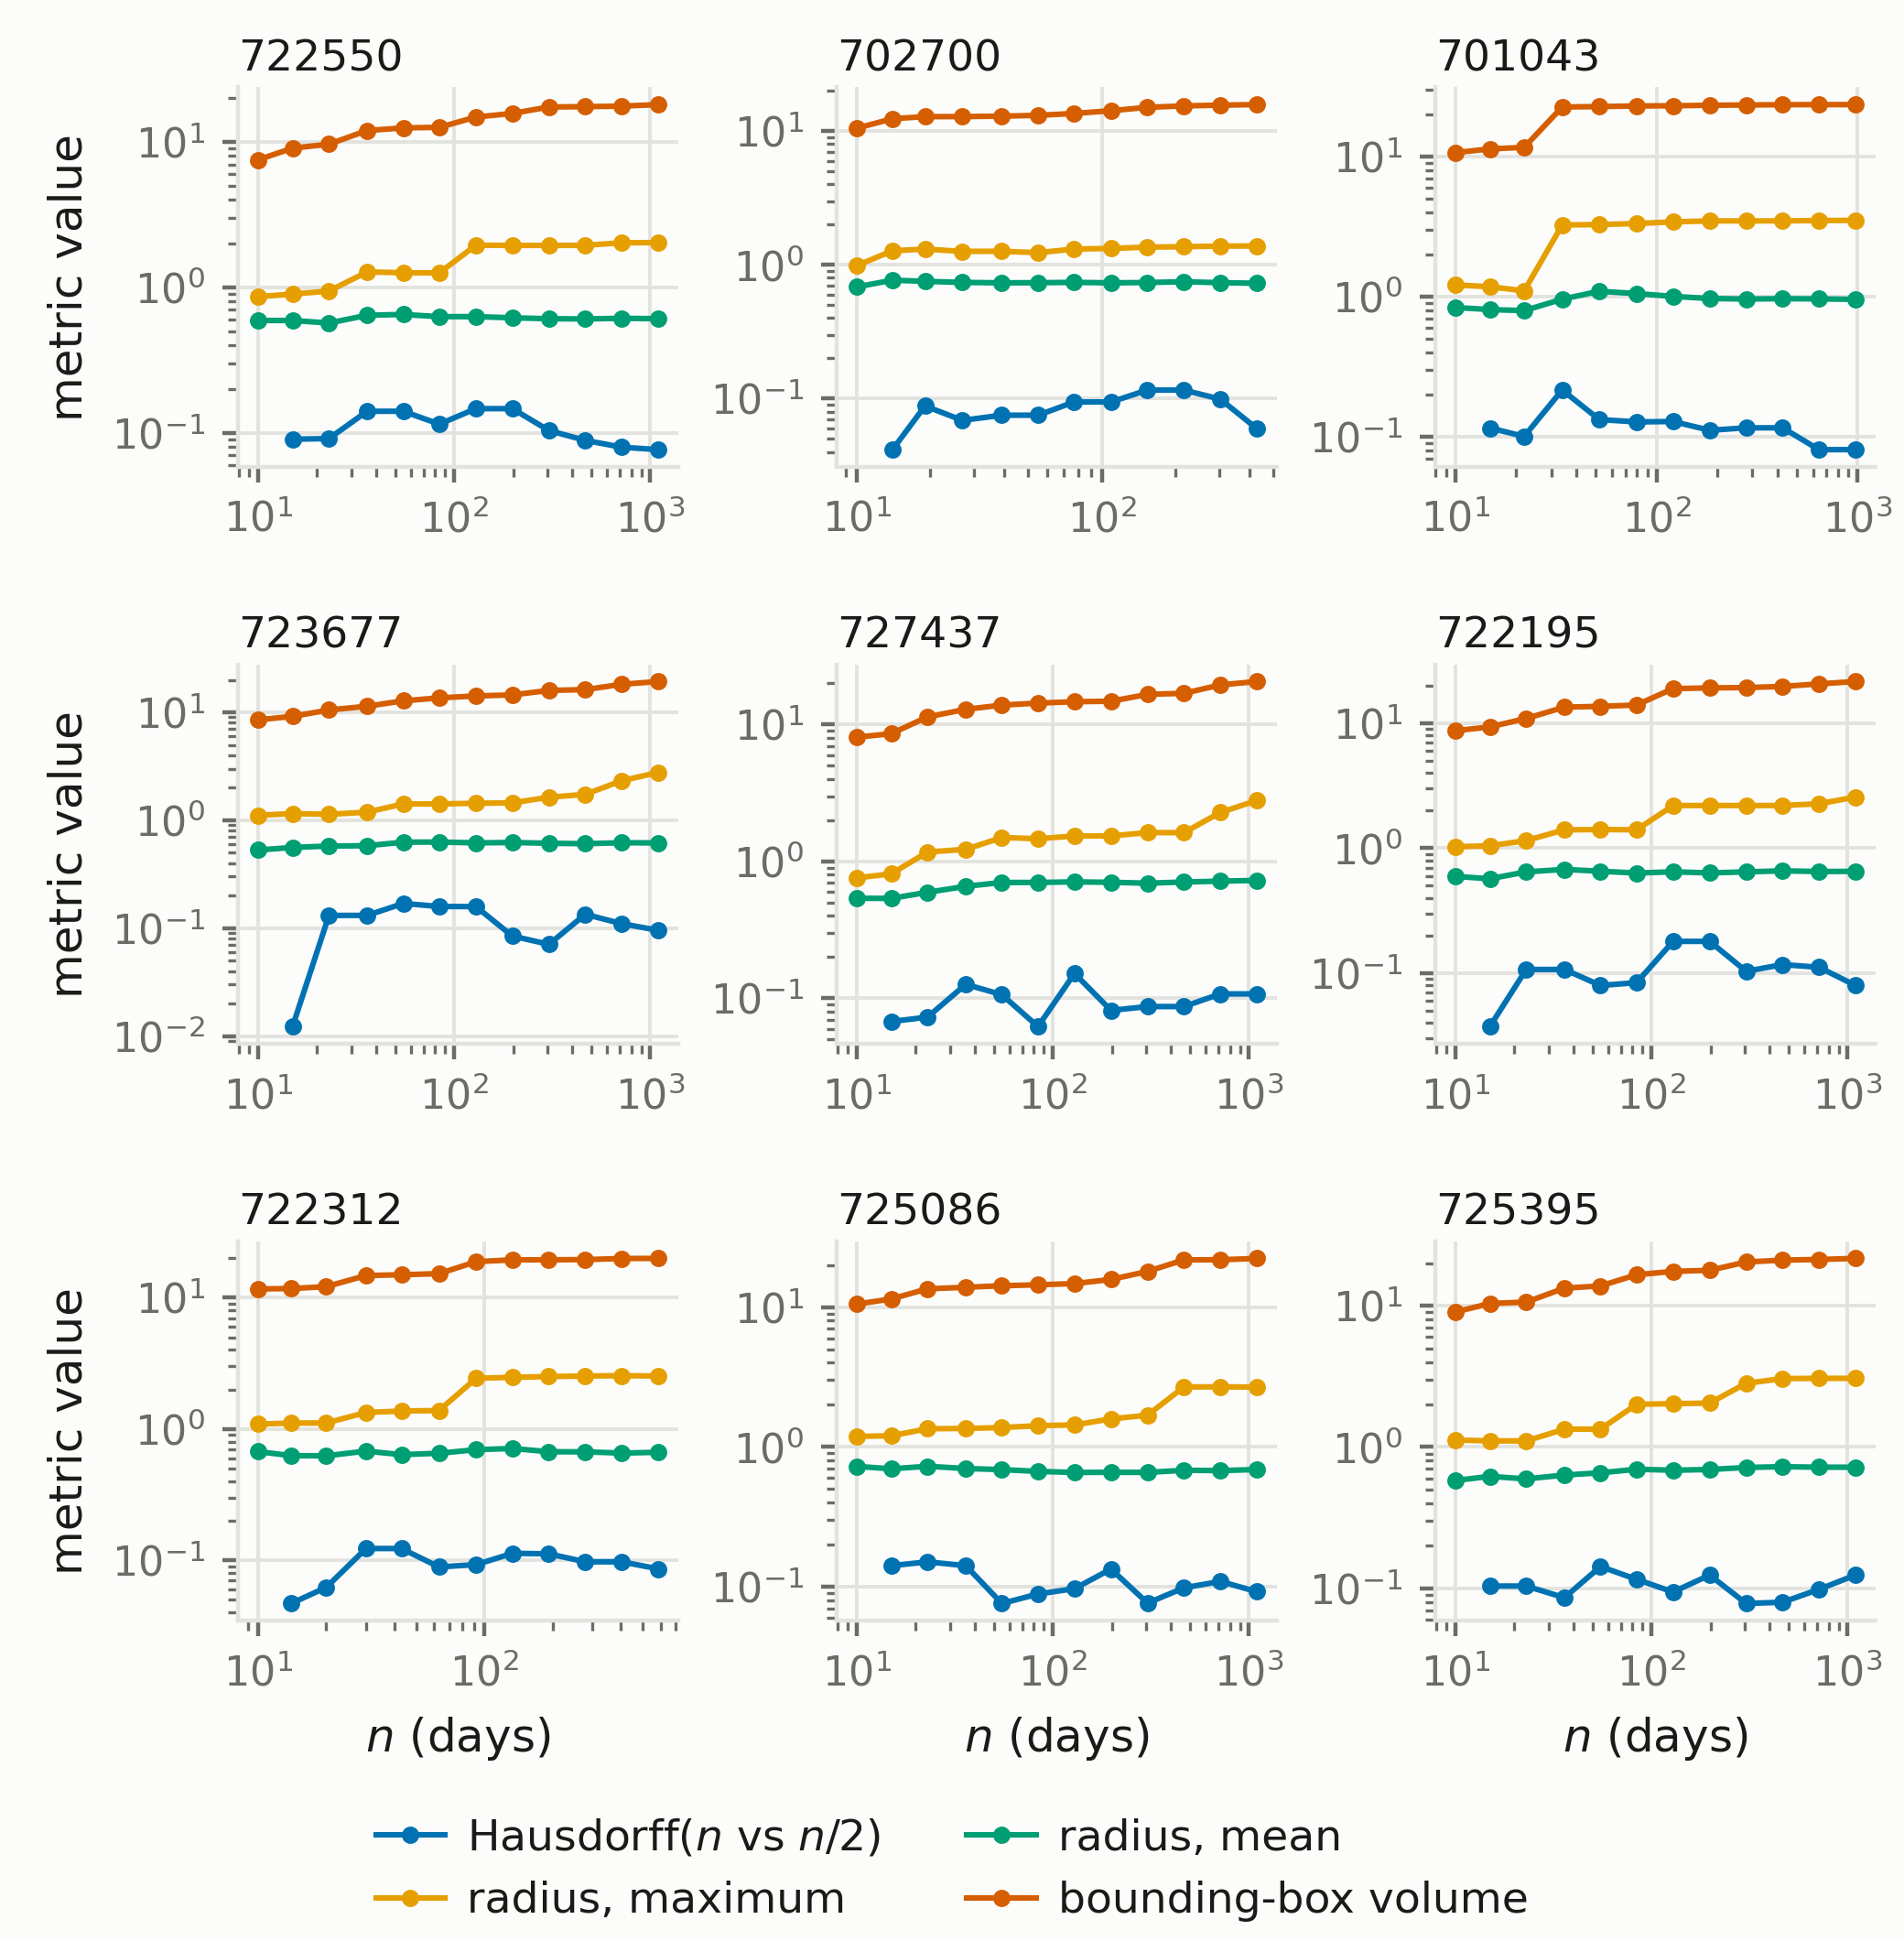
\includegraphics[width=0.8\textwidth]{nsrdb_manifold_saturation_grid.png}
  \caption{\small Geometric saturation curves for multiple NSRDB solar stations. 
  Each panel represents a different geographical location. The mean-radius
  curve flattens consistently across sites; the maximum radius, plotted
  alongside, does not, and no claim is made from it.}
  \label{fig:nsrdb_manifold_saturation_grid} 
\end{figure}


To summarise this behaviour quantitatively across a larger random sample,
we defined an \emph{operational saturation scale} $n_{\mathrm{sat}}$ for
each station using the mean-radius curve. Specifically, $n_{\mathrm{sat}}$
was taken as the first sample size at which the relative change in mean
radius between successive steps fell below 5\% for two consecutive
steps. Under this criterion, the median saturation scale across the
sample was 22 days, with 68.75\% of stations saturating by 30 days and
81.25\% by 40 days. These values confirm that for fixed-site solar irradiance, the mean-radius estimate
stabilises at the specified tolerance after observing only a few tens of daily
profiles. We emphasise that it is the statistical estimate that converges rapidly;
this does not imply that the absolute geometric support has been exhaustively bounded.

\begin{table}[!htbp]
\centering

\begin{minipage}[t]{0.44\textwidth}
\centering
\small
\vspace{25pt}
\begin{tabular}{lc}
\toprule
\textbf{Statistic} & \textbf{Value} \\
\midrule
Number of stations & 80 \\
Mean $n_{\mathrm{sat}}$ & 29.32 days \\
Std. dev. & 27.88 days \\
Median $n_{\mathrm{sat}}$ & 21.5 days \\
25th percentile & 10 days \\
75th percentile & 36 days \\
Minimum & 10 days \\
Maximum & 192 days \\
Fraction with $n_{\mathrm{sat}} \leq 30$ & 66.25\% \\
Fraction with $n_{\mathrm{sat}} \leq 40$ & 81.25\% \\
\bottomrule
\end{tabular}


\vspace{1.5mm}
\textbf{(a)} Summary statistics for $n_{\mathrm{sat}}$.
\end{minipage}
\hfill
\begin{minipage}[t]{0.50\textwidth}
\centering
\vspace{0pt}
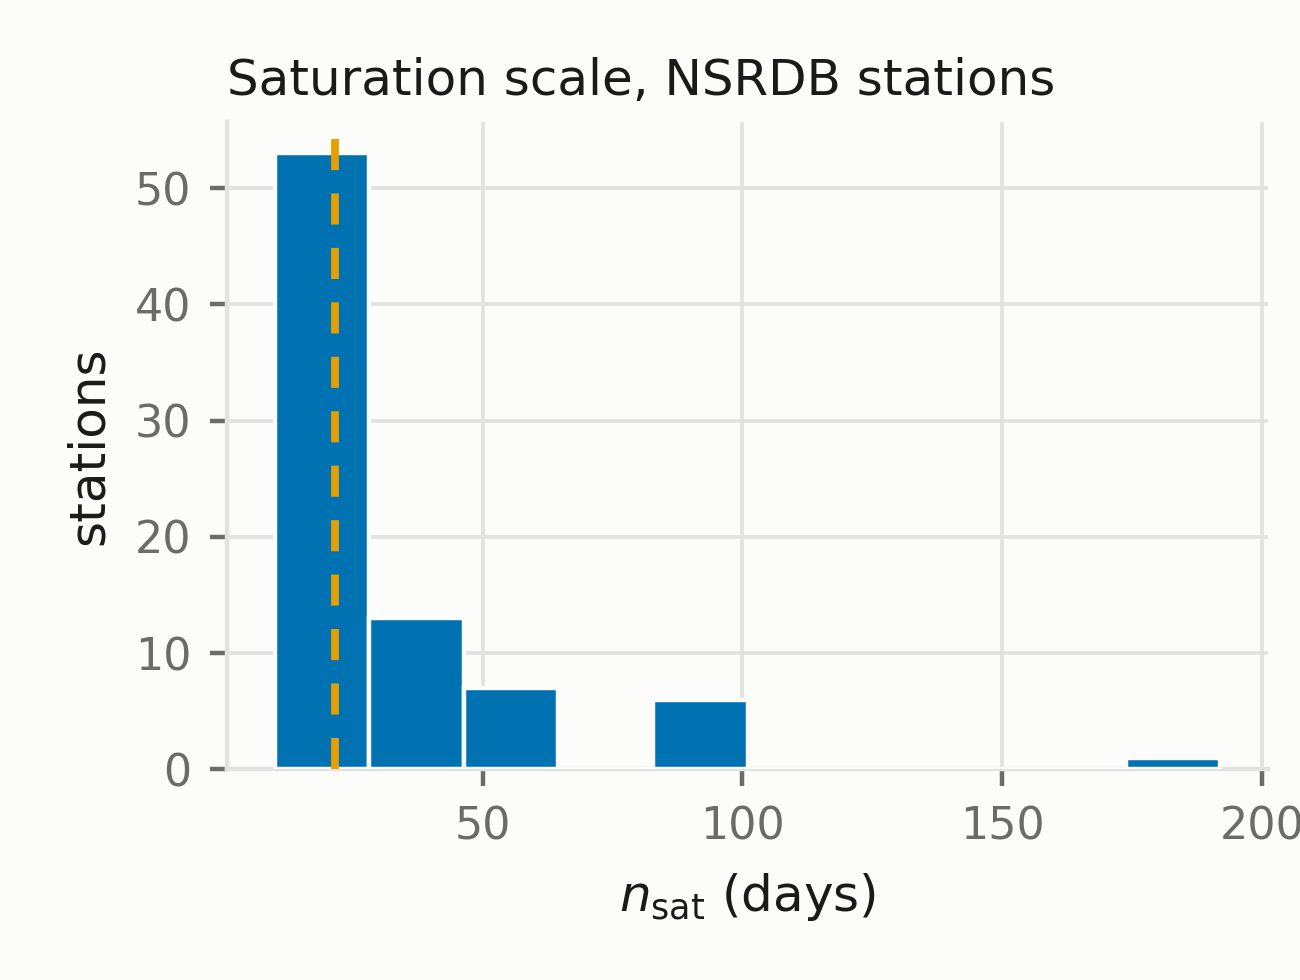
\includegraphics[width=\textwidth,height=0.30\textheight,keepaspectratio]{nsrdb_manifold_saturation_distribution.png}
\label{fig:nsrdb_nsat_distribution}
\vspace{1.5mm}
\textbf{(b)} Histogram of $n_{\mathrm{sat}}$ across stations.
\end{minipage}

\caption{\small Distribution of the operational saturation scale
$n_{\mathrm{sat}}$ across the $N=80$ NSRDB stations of the archive. The
left panel reports aggregate statistics, the right panel the distribution,
with the median dashed. Most sites saturate within a few tens of daily
profiles, and there is a right tail: one station reaches $192$ days. These four multi-site figures and the two tables beside them are regenerated by \texttt{src/figure\_multisite.py}, which ports the pipeline out of the notebook it lived in. Two things changed in the port and both are about reproducibility. The sample ordering is now seeded per station: the estimator takes the first $n$ at which the mean radius changes by less than five per cent twice running, and that value depends on the order in which a station's days are presented, so the unseeded sweep these numbers were first computed with could not be reproduced. And the Hausdorff point at the smallest $n$, where the subsample and the sample coincide, is left undefined rather than plotted at $10^{-14}$, where it set the vertical scale of every panel.}
\label{tabfig:nsrdb_nsat_summary}
\end{table}

Although the distribution exhibits a visible right tail, its bulk is
concentrated in the regime of a few tens of daily profiles. Thus, the
representative saturation scale for fixed-site daily irradiance remains
small even in the presence of occasional late-saturating stations.

\section{Multi-site validation on NOAA tidal manifolds}\label{app:tides_multisite}

\paragraph{Where it deviates, and whether we anticipated it.}
The ordering is not the predicted one and we did not expect it to be. Galveston
is last as predicted and Anchorage and Boston exchange the first two places. The
three stations that fall furthest short --- San Francisco by four places, San
Diego by two, Honolulu by one, all in the direction of \emph{less} compact than
predicted --- are exactly the three named in advance under the mixed-regime
cause: where diurnal constituents are strong the lunar day alternates between
one and two high waters, so the window contains two shapes rather than one.
That the declared failure mode is the one that fired, on the stations it named,
is the part of this we did not have to argue for afterwards.

The diagnostic we thought most likely does \emph{not} account for them, and we
report that too. We had declared that a jumping fiducial would show up as a
bimodal distribution of the second high water's position after alignment.
Sarle's coefficient exceeds the $5/9$ threshold at San Diego ($0.809$),
Atlantic City ($0.740$), Key West ($0.675$) and Honolulu ($0.572$) --- but
Atlantic City and Key West moved \emph{toward} the prediction, not away from it,
and San Francisco, which deviates most, does not trigger the diagnostic at all
($0.495$). The diagnostic fires, and where it fires does not line up with where
the prediction failed. It is not the explanation.

\paragraph{The mechanism that fired is also a rival explanation.}
Cause C2 was declared as a deviation mechanism: where the diurnal constituents
are strong the lunar day alternates between one and two high waters, so the
window holds two shapes rather than one. It fired, on the stations it named.
But a mechanism that widens some classes is also a candidate explanation of the
whole ordering, and the pre-registration did not ask whether the two could be
told apart. We ask it here.

We measure the inequality directly: within each lunar day, the gap between the
highest level in each half of the window, divided by that window's range, taken
as the median over days. This is our operationalisation and not the
harmonic-analysis definition, and it is declared rather than tuned. It orders
the stations as the physics says it should --- Anchorage ($0.044$) and Boston
($0.091$), the large-range semidiurnal pair, are the most symmetric; Honolulu
($0.236$) and Key West ($0.250$), small and mixed, the least.

Against $\varepsilon$ it gives $\rho = +0.517$: more diurnal inequality, larger
$\varepsilon$, in the direction the mechanism predicts. The declared amplitude
variable gives $-0.667$. Combining them --- range scaled by symmetry --- gives
$-0.583$, weaker than range alone, so the combination buys nothing.

\textbf{With nine stations these two cannot be separated, and we do not claim
to have separated them.} Large-range stations tend to be semidiurnal, so
amplitude and symmetry are not independent across this sample, and the
difference between a rank correlation of $0.52$ and one of $0.67$ on nine
points is not a quantity anyone should reason from. What the pre-registered
test established is that $\varepsilon$ falls with tidal range on these nine
stations; what it did not establish, and could not have, is that the range is
what does the work. A design that could separate them would need stations
chosen to break the association --- large range and strongly mixed, small range
and strongly semidiurnal --- and choosing them now, after seeing this, would be
the same error the pre-registration exists to prevent.

We report it because the diagnostic that found this limit is one the
pre-registration itself declared, and a named cause that is measured only when
it flatters the result is not a control.

\paragraph{An admission, and what follows from it.}
Reading that result is what showed us that the declared C5 diagnostic does not
test what we said it tested. We did not notice before running the experiment.
Repairing the instrument now and re-measuring would be choosing an alignment
rule while looking at the answer, so we did not: \textbf{the number in this
section is the pre-registered instrument's and is not replaced}. A single
corrected fiducial --- cross-correlation against a template, two iterations, as
an ECG beat is aligned --- was specified in writing before it was run, with no
variants tried and a commitment to report it whatever it said. It gives
$\rho = -0.633$, which still meets the criterion, does not rescue the ordering,
and is slightly weaker than the original. It is in
\ref{app:noaa_multisite}, where it was committed to go.

\paragraph{The alignment is not a convenience.}
Sea level on the MSL datum is a zero-mean oscillation, so two lunar days sampled
at different phase are nearly orthogonal under the cosine metric and what the
measurement returns is the phase of the recording rather than the shape of the
tide. Removing the fiducial altogether makes this concrete: $\varepsilon$ rises
from between $0.02$ and $0.27$ to between $0.43$ and $1.06$, the compression
against the surrogate collapses to $1.0\times$ at every station --- the real
tides become exactly as expensive to cover as a signal with their spectrum ---
and the pre-registered correlation \emph{inverts}, from $-0.633$ to $+0.633$ on
the same stations. Declaring the time origin is not a preprocessing detail
here. It is the difference between measuring a phenomenon and measuring when the
recorder happened to start.



\label{app:noaa_multisite}

Two measurements on tidal data appear in this paper and they are not the same
measurement. Section~\ref{sec:results-tides} reports the pre-registered one: one
lunar day, aligned to high water, on the MSL datum, amplitude not normalised.
The saturation curves in this appendix come from an earlier pipeline --- $24$-hour
calendar days, min--max scaled to the unit interval, on an hourly grid --- and
are retained as an independent check under a different realisation and a
different normalisation, which is why their numbers are not the body's and why
their station list is not identical. The corrected fiducial committed to in
Section~\ref{sec:results-tides} is reported at the end of this appendix.

To verify that the rapid geometric saturation observed in geophysical signals is a general property of tidal dynamics rather than a site-specific artefact, we extended our analysis across multiple coastal environments. We utilised the NOAA Center for Operational Oceanographic Products and Services (CO-OPS) API to retrieve verified hourly water-level data from a geographically diverse set of stations, including Pacific (Honolulu, San Francisco), Atlantic (Boston, Charleston), and Gulf Coast (Galveston) locations. 
For each station, we constructed a daily tidal manifold using a pipeline analogous to the one described in the main text: the continuous sea-level time series was segmented into 24-hour calendar days, reindexed to a fixed hourly grid, and processed to resolve any missing observations via linear interpolation. To isolate the topological structure of the tidal harmonics from site-specific tidal ranges and mean sea-level offsets, each daily curve was normalised using min-max scaling, mapping the values to the unit interval $[0, 1]$. Each day was thus represented as a vector in $\mathbb{R}^{24}$, and the collection of these vectors defined the station-specific tidal manifold.
To test whether the geometry saturates generically across different harmonic regimes (e.g., diurnal, semi-diurnal, and mixed tides), we computed the same saturation curves used throughout this work: the internal Hausdorff discrepancy, the maximum radius, the mean radius, and the summed coordinate extent as functions of sample size $n$. Figure~\ref{fig:tides_multisite_saturation} shows these curves for the 9 selected stations. In every case the mean radius flattens quickly, and faster than in the solar or physiological domains. The maximum radius is plotted beside it and does not settle in the same way; only the mean-radius curve supports the reading given here, and only it is used for the operational scale below. This is consistent with astronomical forcing dominating the local variability, though the sample of nine stations does not identify which harmonic regime is responsible.

\begin{figure}[ht]
  \centering
  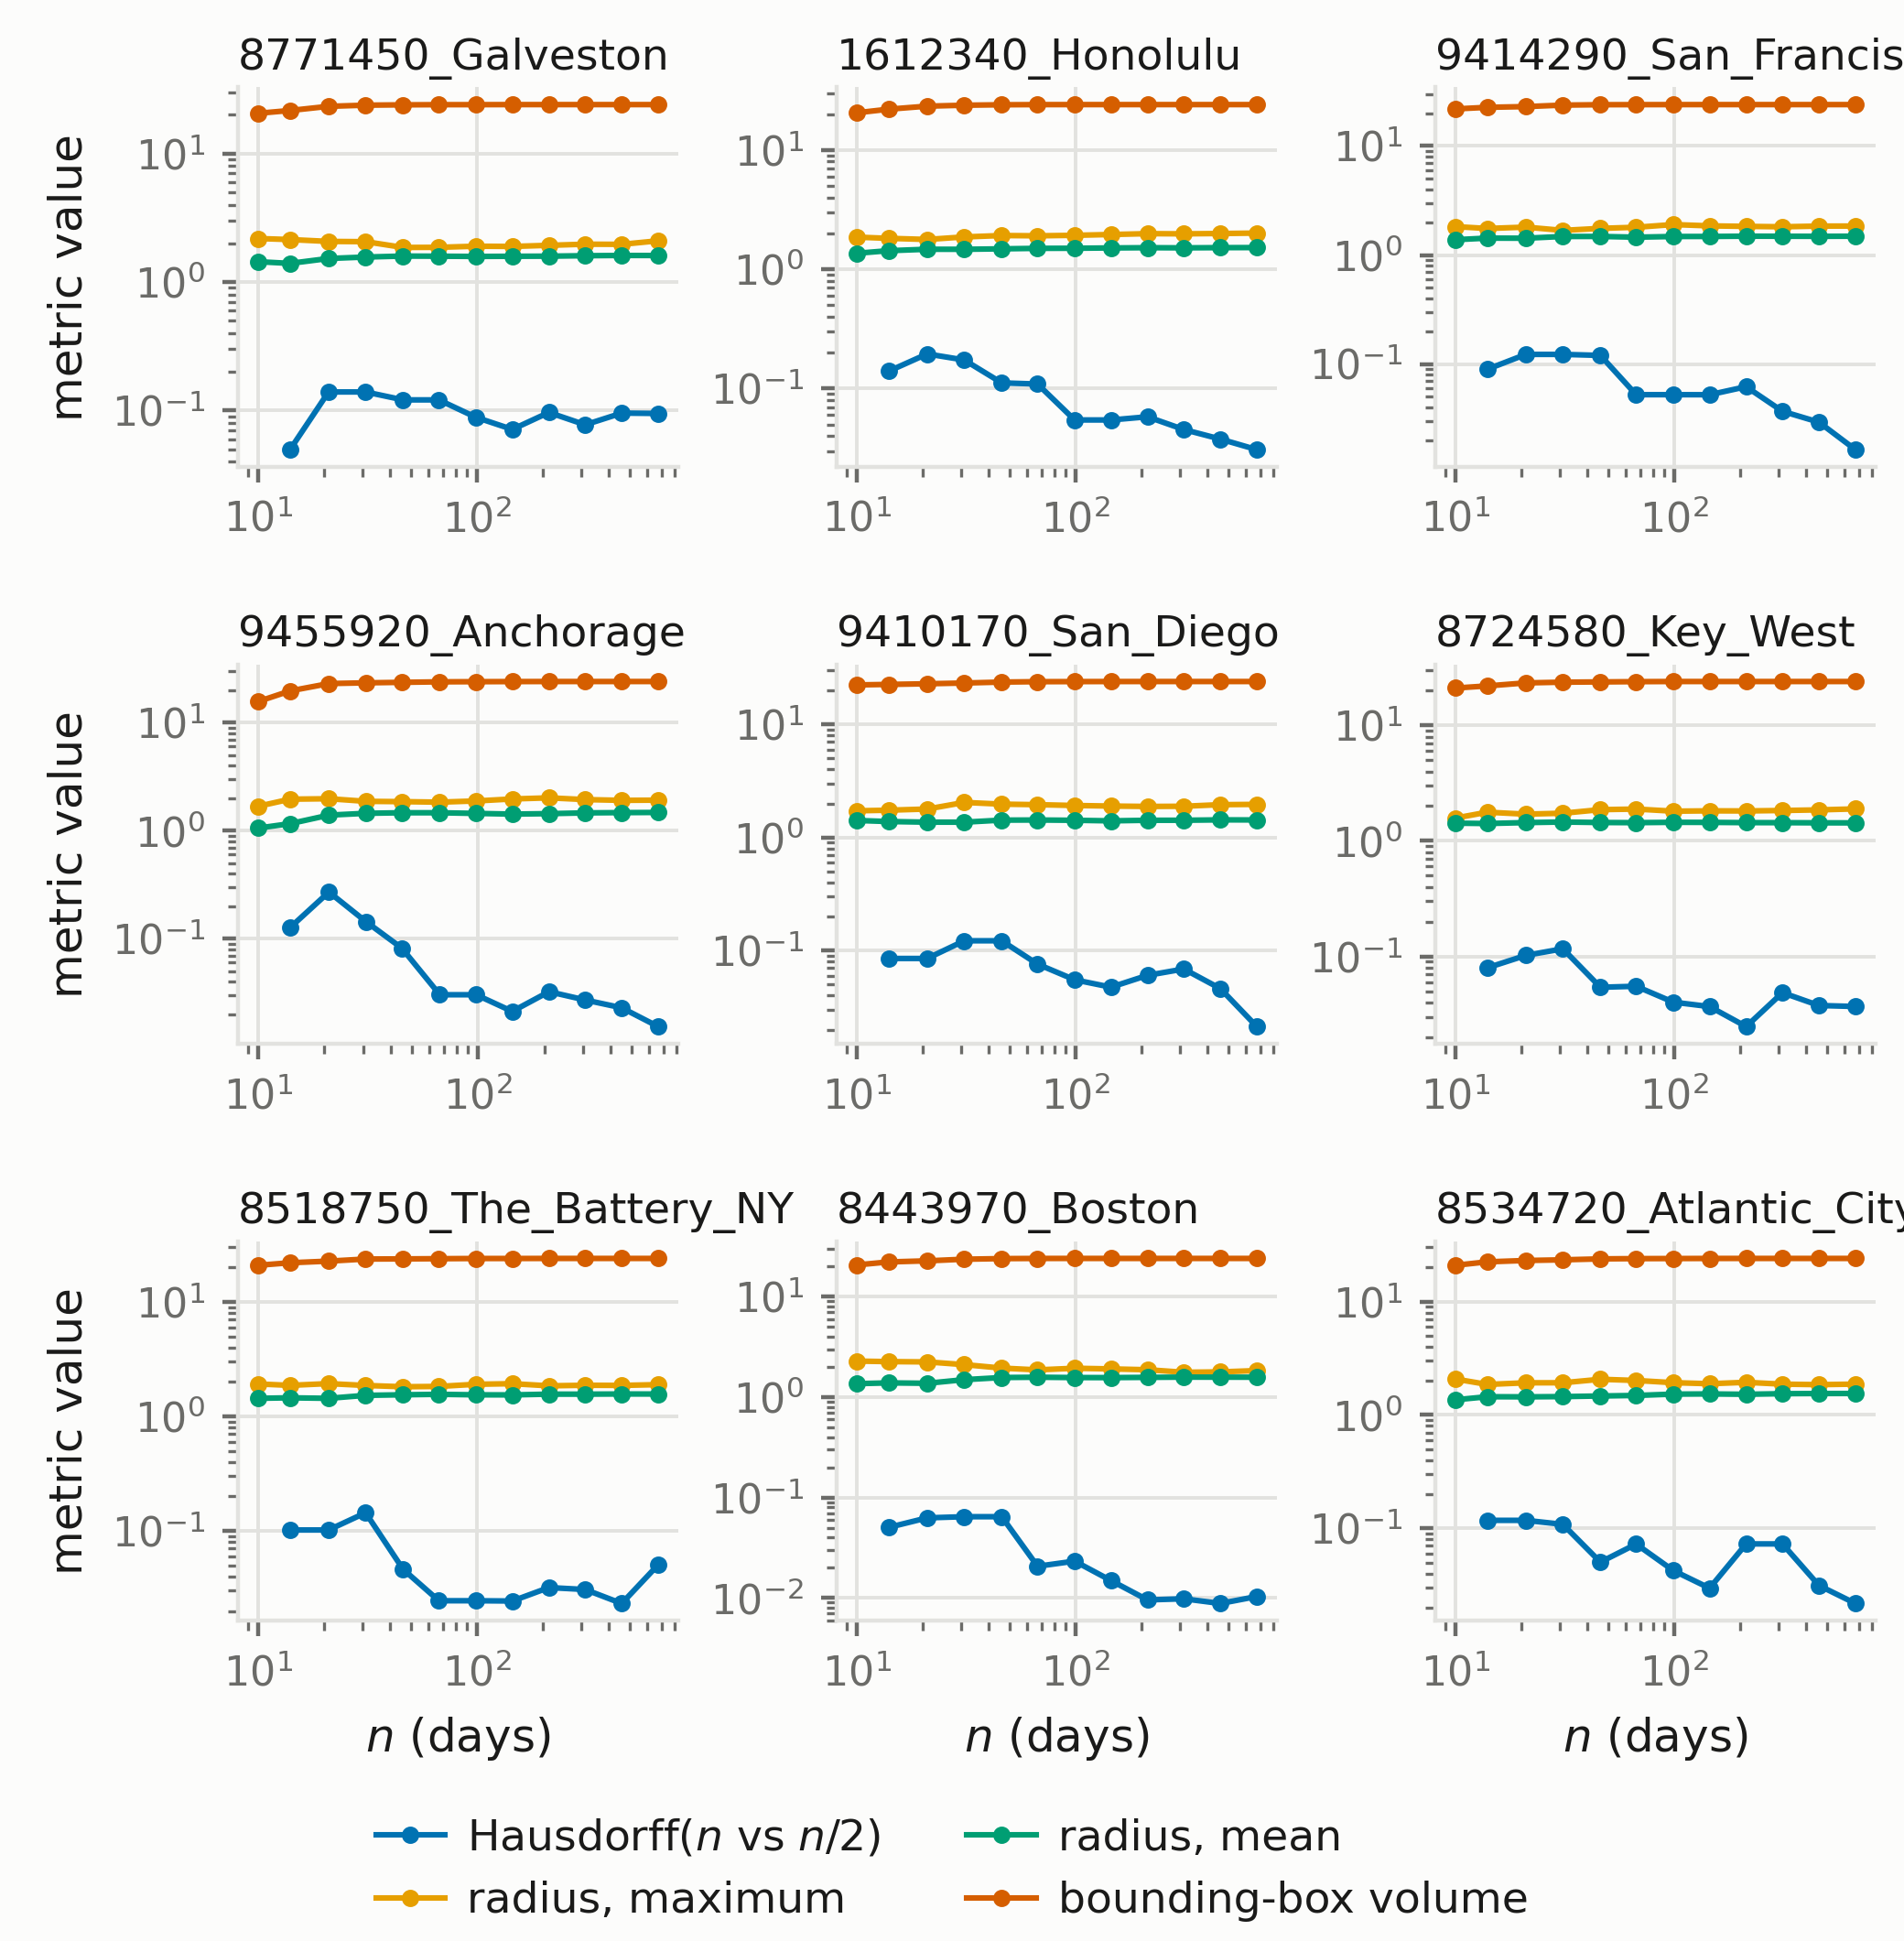
\includegraphics[width=0.8\textwidth]{tides_manifold_saturation_grid.png}
  \caption{\small Geometric saturation curves for multiple NOAA tidal stations. Each panel corresponds to a different coastal station. The mean radius flattens early at every site. Note that these panels use the older multi-site pipeline described in this appendix --- calendar days, min--max scaling, $\mathbb{R}^{24}$ --- and not the observable declared in Section~\ref{sec:results-tides}, whose min--max normalisation is the one the body reports as a defect because it erases the spring--neap variation. They are shown as a breadth check across sites, not as evidence about compactness, which the framework assumes rather than tests.}
  \label{fig:tides_multisite_saturation} 
\end{figure}

To summarise this behaviour quantitatively, we applied the operational saturation scale $n_{\mathrm{sat}}$ (defined as the first sample size where the relative change in mean radius stays below 5\% for two consecutive steps). The aggregate statistics, reported in Table~\ref{tabfig:tides_nsat_summary}, reveal a remarkably efficient characterisation of the manifold: the median saturation scale is only 10 days --- less than two weeks of data before the mean-radius estimate stops moving at that tolerance. It is an estimate settling, not the geometry being resolved.

\begin{table}[!htbp]
\centering
\begin{minipage}[t]{0.44\textwidth}
\centering
\small
\vspace{25pt}
\begin{tabular}{lc}
\toprule
\textbf{Statistic} & \textbf{Value} \\
\midrule
Number of stations & 9 \\
Mean $n_{\mathrm{sat}}$ & 13.33 days \\
Std. dev. & 4.66 days \\
Median $n_{\mathrm{sat}}$ & 10 days \\
25th percentile & 10 days \\
75th percentile & 14 days \\
Minimum & 10 days \\
Maximum & 21 days \\
Fraction with $n_{\mathrm{sat}} \leq 15$ & 77.78\% \\
Fraction with $n_{\mathrm{sat}} \leq 21$ & 100\% \\
\bottomrule
\end{tabular}


\vspace{1.5mm}
\textbf{(a)} Summary statistics for $n_{\mathrm{sat}}$.
\end{minipage}
\hfill
\begin{minipage}[t]{0.50\textwidth}
\centering
\vspace{0pt}
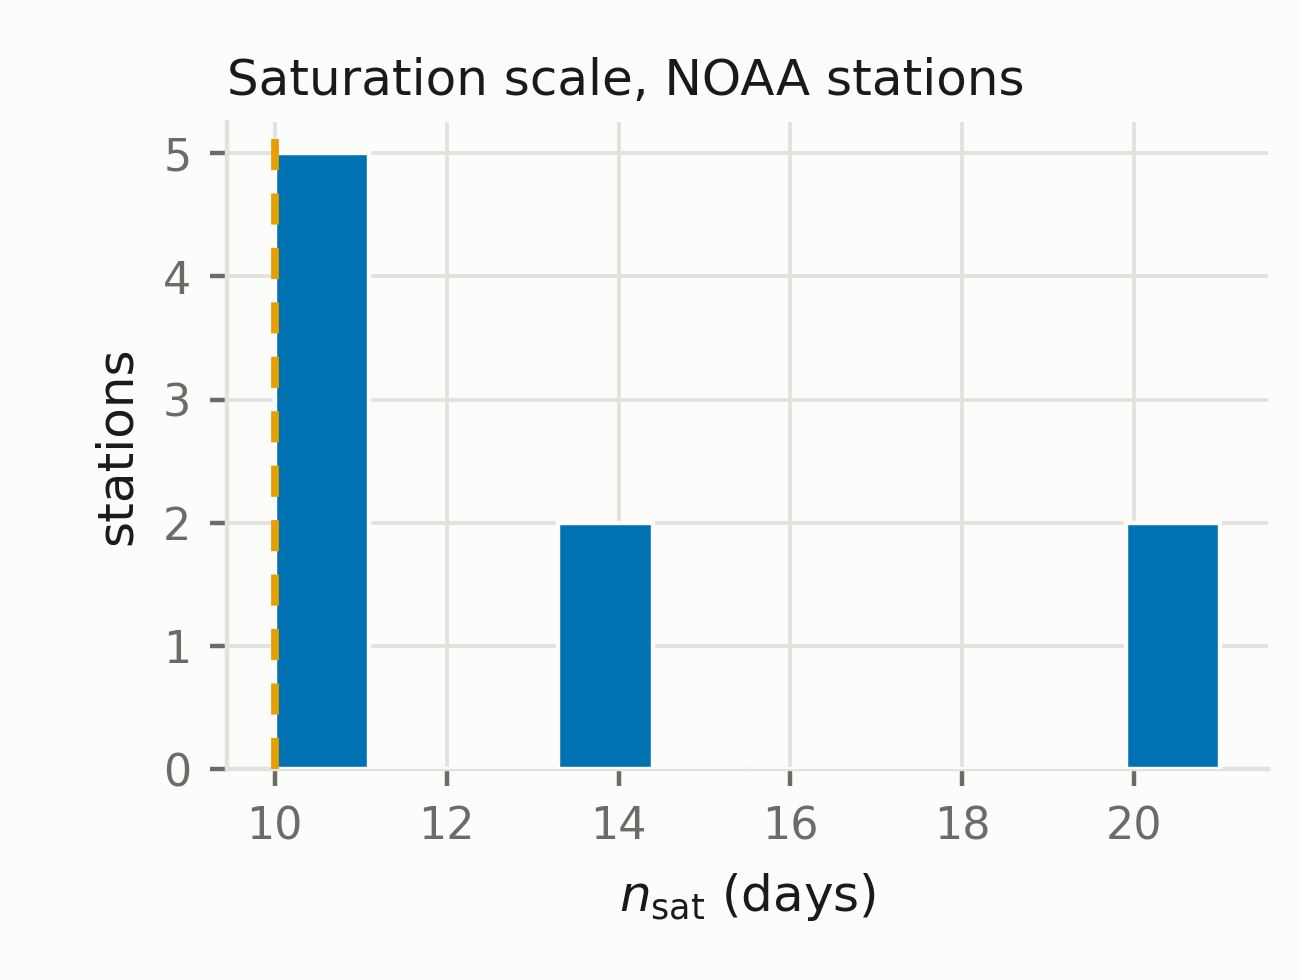
\includegraphics[width=\textwidth,height=0.30\textheight,keepaspectratio]{tidal_manifold_saturation_distribution.png}

\vspace{1.5mm}
\textbf{(b)} Histogram of $n_{\mathrm{sat}}$ across tidal stations.
\end{minipage}

\caption{\small Distribution of the operational saturation scale
$n_{\mathrm{sat}}$ across $N=9$ NOAA tidal stations, with the median dashed.
The distribution is shifted to the left compared to the solar one: the median
is ten days and the largest value in the sample is twenty-one. The
reproducibility note in Table~\ref{tabfig:nsrdb_nsat_summary} applies to this
figure and this table as well.}
\label{tabfig:tides_nsat_summary}
\end{table}

The contrast between these results and the solar manifolds is instructive. While solar irradiance is subject to stochastic atmospheric interference (clouds) that introduces late-stage variability, tidal levels are governed by the high-precision determinism of gravitational mechanics. Consequently, an observer's estimate of the tidal manifold settles rather more than twice as fast as its estimate of the solar one, a median of ten days against twenty-one and a half. These findings support the central thesis of this work: signal families governed
by strong deterministic constraints tend to exhibit rapidly saturating empirical
manifolds under the adopted representation, metric, and sampling protocol.
%--------------------------------------------------------
% PM GENERATOR
%--------------------------------------------------------

\subsection{The corrected fiducial, as committed}
\label{app:tides-fiducial}

Section~\ref{sec:results-tides} records that the C5 diagnostic we declared in
advance does not test what we said it tested, and that we did not notice before
running the experiment. This appendix carries what we committed to in writing at
that point: one corrected alignment rule, specified before it was run, with no
variants tried, reported whatever it says, and placed here rather than in the
body because the body's number must remain the pre-registered instrument's.

The rule is cross-correlation against a template, which is how an ECG beat is
aligned in practice: the initial template is the mean of the days aligned by
per-block \texttt{argmax}; each day is shifted to the lag maximising its
cross-correlation with the template; the template is recomputed and the shift
repeated, twice, fixed. It does not depend on detecting peaks.

Table~\ref{tab:fiducial} reports it beside the pre-registered fiducial and beside
no fiducial at all. Three readings follow, and the third is the one that matters.

The corrected fiducial tightens every station --- $\varepsilon$ falls at all nine
--- which is what a better alignment should do. It does \emph{not} rescue the
prediction: $\rho$ moves from $-0.667$ to $-0.633$, still inside the criterion
declared in advance but slightly weaker, and the stations that deviated most
continue to deviate. Had we swapped it into the body it would have been a
marginally worse result obtained by a rule chosen after seeing the answer, which
is the precise thing the commitment was written to prevent.

The bimodality column is the C5 diagnostic. It exceeds Sarle's $5/9$ threshold at
four stations, and those four are not the ones that broke the prediction: two of
them, Atlantic City and Key West, came out \emph{more} compact than predicted,
and San Francisco, which deviates furthest, does not trigger it. A diagnostic
that fires where the prediction succeeded and stays silent where it failed is not
a diagnostic of that failure. We report it as declared and we do not use it.

Removing the fiducial altogether is the third column, and it is not a subtle
effect. Sea level on the MSL datum is a zero-mean oscillation, so two lunar days
sampled at different phase are close to orthogonal under the cosine metric:
$\varepsilon$ rises by a factor of between four and fifty, and the
pre-registered correlation inverts to $+0.633$. Without a declared time origin the measurement
returns the phase of the recording, not the shape of the tide.

\begin{table}[!htbp]\centering\small
\fitwidth{\begin{tabular}{lrrrrr}
\toprule
& range & \multicolumn{3}{c}{$\varepsilon$ by fiducial} & bimodality \\
\cmidrule(lr){3-5}
station & (m) & pre-registered & corrected & none & (C5) \\
\midrule
Boston & 3.117 & 0.0228 & 0.0161 & 0.9982 & 0.268 \\
Anchorage & 8.858 & 0.0658 & 0.0289 & 1.0136 & 0.261 \\
The Battery NY & 1.569 & 0.0982 & 0.0645 & 0.9492 & 0.193 \\
Atlantic City & 1.432 & 0.1034 & 0.0752 & 0.9170 & \textbf{0.740} \\
Key West & 0.578 & 0.1198 & 0.0982 & 0.6165 & \textbf{0.675} \\
San Diego & 1.791 & 0.1412 & 0.1101 & 1.0482 & \textbf{0.809} \\
San Francisco & 1.808 & 0.1533 & 0.1105 & 1.0628 & 0.495 \\
Honolulu & 0.598 & 0.1899 & 0.1685 & 1.0417 & \textbf{0.572} \\
Galveston & 0.531 & 0.2677 & 0.1182 & 0.4260 & 0.471 \\
\midrule
Spearman $\rho$ & & $-0.667$ & $-0.633$ & $+0.633$ & \\
\bottomrule
\end{tabular}
% Bimodality is Sarle's coefficient on the position of the
%   second high water after alignment; bold exceeds 5/9.
% The pre-registered criterion was rho <= -0.6.
}
\caption{\small The three fiducials and the C5 diagnostic. $\varepsilon$ under
the pre-registered alignment (per-block \texttt{argmax}), under the corrected one
(template cross-correlation, two iterations, specified before running), and under
none. Bimodality is Sarle's coefficient on the position of the second high water
after alignment, in bold where it exceeds $5/9$. The pre-registered criterion was
$\rho \le -0.6$ on the coefficient, not on a $p$-value.}
\label{tab:fiducial}
\end{table}

\section{Pooling the point-machine populations}
\label{app:pm-pooling}

Section~\ref{sec:datasets} pools four nominal populations --- two machines, two
directions --- into the single point-machine domain used throughout this paper.
This appendix is the measurement behind that decision. It is a question about
the asset rather than a claim of this work, and it earns a place here for one
reason: the paper's point-machine numbers are computed on the union, and a
reader is entitled to the evidence that the union is one thing.

These tables come from their own run (\texttt{pm\_sets.py} and
\texttt{pm\_pooling.py}), not from the run that produced the tables in the
body. Each manoeuvre is the instantaneous power envelope on $160$ points under
the $\ell_2$ quotient, distance is cosine, and every figure is a mean over ten
repetitions drawing $600$ manoeuvres from each set.

\subsection*{Two measurements, which can disagree}

For an ordered pair $(A,B)$ we draw $2m$ manoeuvres from $A$ and $m$ from $B$,
form the mixture of $m$ from $A$ with the $m$ from $B$, and cover both the
mixture and the $2m$ of $A$ alone with a greedy $\varepsilon$-net:
\[
  \rho(A,B) \;=\; |S(\text{mixture})| \,/\, |S(A, 2m)| .
\]
If $B$ falls inside the balls already centred on $A$'s exemplars the mixture
needs no new ones and $\rho \approx 1$; if it does not, every uncovered
manoeuvre forces a new exemplar. Alongside it we report separability,
$P\!\left(d(a,a') < d(a,b)\right)$, which is $\tfrac12$ when the metric cannot
tell the two sets apart.

Two choices in that design carry the experiment. First, \textbf{the tolerance
is $A$'s own within-set median, never the mixture's}: a mixture of two
different populations has larger typical distances and therefore a larger
tolerance, so using the mixture's median would buy a coarser ruler exactly when
heterogeneity is present and would conceal the effect being measured. This was
an error in the first version of the script and it inverted the control.
Second, \textbf{every pair is measured in both directions}, because with
tolerances differing by a factor of three a single direction confounds
\emph{these sets differ} with \emph{the reference happened to be the tight one}.

\subsection*{Calibration}

The diagnostic is run first on controls whose answer is known: two compact
manifolds on the same three-dimensional subspace, and two on different
subspaces, at matched sample size and noise.

\begin{center}\small
\begin{tabular}{lrr}
\toprule
control & $\rho$ & separability \\
\midrule
same manifold & 0.94 & 0.495 \\
different manifolds & 1.73 & 1.000 \\
\bottomrule
\end{tabular}

\end{center}

These two poles are the scale on which everything below is read. A diagnostic
not shown to separate the two cases it exists to separate is not a diagnostic.

\subsection*{Result, pairwise}

\begin{center}\small
\begin{tabular}{lrrrrl}
\toprule
pair & $\bar\rho$ & asym. & separability & of the way to ``two'' & kind \\
\midrule
J1 r$\to$n $+$ J2 r$\to$n & 1.09 & 0.20 & 0.577 & 19\% & same direction, different unit \\
J1 n$\to$r $+$ J2 n$\to$r & 1.15 & 0.17 & 0.546 & 27\% & same direction, different unit \\
J1 n$\to$r $+$ J2 r$\to$n & 1.28 & 0.45 & 0.741 & 43\% & cross \\
J2 n$\to$r $+$ J2 r$\to$n & 1.28 & 0.33 & 0.666 & 43\% & same unit, both directions \\
J1 r$\to$n $+$ J2 n$\to$r & 1.29 & 0.39 & 0.770 & 45\% & cross \\
J1 n$\to$r $+$ J1 r$\to$n & 1.30 & 0.29 & 0.846 & 46\% & same unit, both directions \\
\bottomrule
\end{tabular}

\end{center}

No pair travels past halfway to the ``different manifolds'' pole. Pooling any
two costs at most thirty per cent more exemplars than covering one of them at
twice the sample size.

The two same-direction pairs are the informative rows. Their separabilities are
$0.546$ and $0.578$ against a floor of $0.500$: take two manoeuvres of one unit
and one of the other, and the two from the same unit are the closer pair
$54.6\%$ of the time where an instrument blind to unit identity would give
$50\%$. There \emph{is} a unit signature --- both figures sit above the floor,
and in the same direction rather than scattered about it --- and it is small,
and its size is now known rather than assumed. \textbf{The nominal form is a
property of the mechanism type and not of the individual unit}, which is what
makes a nominal model built on one machine transferable to another of the same
design.

Two qualifications travel with that. These are two units from one archive, so
the claim is \emph{these two are interchangeable}, not \emph{units of this type
are}. And the direction effect is the larger of the two: every pair that
changes direction sits above both pairs that do not, in both measurements,
without exception. What that asymmetry is --- locking geometry at the two
endpoints, a return spring, drainage, asymmetric wear --- the experiment cannot
say, and we do not guess.

\subsection*{Result, all four at once}

The pairwise test asks whether $B$ falls inside the balls centred on $A$. A
second and independently written measurement asks the blunter question: what
does covering all four together cost? Every set is measured at every tolerance,
so the comparison is at fixed scale; read down a column.

\begin{center}\small
\begin{tabular}{lrrrrr}
\toprule
$|S|$ at the tolerance of $\to$ & J1 n$\to$r & J1 r$\to$n & J2 n$\to$r & J2 r$\to$n & all four \\
 & 0.0382 & 0.0127 & 0.0387 & 0.0266 & 0.0514 \\
\midrule
J1 normal $\to$ reverse & 5.24 & 11.34 & 5.20 & 6.50 & 3.94 \\
J1 reverse $\to$ normal & 4.76 & 8.76 & 4.74 & 5.44 & 3.62 \\
J2 normal $\to$ reverse & 5.20 & 12.42 & 5.16 & 7.20 & 4.26 \\
J2 reverse $\to$ normal & 3.44 & 8.32 & 3.36 & 4.38 & 2.76 \\
\midrule
all four together & 5.80 & 15.54 & 5.76 & 7.60 & 4.82 \\
sum of the four & 18.64 & 40.84 & 18.46 & 23.52 & 14.58 \\
all four $/$ largest & 1.11 & 1.25 & 1.11 & 1.06 & 1.13 \\
\bottomrule
\end{tabular}

\end{center}

Four different manifolds would put the union near the \emph{sum}: a ball
centred in one population covers nothing in another, so the costs add. The
union costs between $1.06$ and $1.25$ times the largest single population at
every one of the five tolerances, and between $0.31$ and $0.38$ times the sum.
Four times the data buys a tenth more exemplars.

\paragraph{One caution, stated so that nobody has to rediscover it.} The
tolerance of the four together is $0.0514$, larger than every individual
tolerance and $1.33$ times the largest. $\varepsilon$ is a median \emph{within}
a set, and a mixture of populations sitting in different places has a larger
median than any of them; a larger tolerance buys a smaller net. That is the
whole of the apparent paradox in the last column, where the four together need
fewer exemplars ($4.82$) than the first population alone ($5.24$). The ruler
changed length; the set did not shrink. Only the fixed-tolerance columns carry
meaning.

\subsection*{The pooled radius converges as the parts do}

Measured on realisations the estimate never saw, as a percentage of where each
set settles.

\begin{center}\small
\begin{tabular}{lrrrrr}
\toprule
set & settles at & $n{=}5$ & $n{=}20$ & $n{=}50$ & $n{=}200$ \\
\midrule
J1 normal $\to$ reverse & 0.02243 & 23.3 & 6.1 & 3.1 & 0.8 \\
J1 reverse $\to$ normal & 0.01005 & 24.5 & 5.1 & 0.6 & 1.9 \\
J2 normal $\to$ reverse & 0.02134 & 34.4 & 2.9 & 0.9 & 1.9 \\
J2 reverse $\to$ normal & 0.01736 & 21.5 & 5.0 & 3.0 & 1.2 \\
all four together & 0.02682 & 21.8 & 7.4 & 1.3 & 0.6 \\
\bottomrule
\end{tabular}

\end{center}

Pooling four populations from two units and two directions does not slow the
convergence. On the largest sample the union is the cleanest of the five. A set
assembled from four sources behaves like one phenomenon under the only
measurement that describes a phenomenon's scale.

\subsection*{Why a ratio near one and a separability above a half are not in
conflict}

They measure different things, and the combination is the informative part.
$\rho \approx 1$ says that at this resolution and this sample size the union
costs no more to cover than either part alone: essentially no manoeuvre of one
population fell outside the balls already centred on the other's exemplars.
That is a statement about covering cost at a stated $\varepsilon$ and $n$, not a
certificate that the two supports coincide --- an $\varepsilon$-net is not used
in this paper to establish that a set has been exhausted. Separability above $\tfrac12$ says the two do not fill that support
\emph{identically} --- there is a systematic displacement between them, and it
is smaller than $\varepsilon$. The sets differ in where they concentrate, not
in what they can reach.

This is the same distinction the body of the paper turns on in
Section~\ref{sec:bulk-boundary}: a covering number is a functional of the
support, a separability is a functional of the measure, and the two are
entitled to disagree. Here they disagree in the direction that says one region,
filled slightly differently by two machines.

\section{The ten concepts of each digit set, separately}
\label{app:digits-per-class}

Section~\ref{sec:results} reports one convergence curve per digit set, and each
of those is an average over the set's ten concepts. An average can hide a
mixture: ten classes that all settle at the same sample size and ten where
half settle immediately and half never do produce similar means, and the
distinction matters, because the paper's claim is about a class and not about
a collection of classes. This appendix separates them.

\begin{figure}[!htbp]
\centering
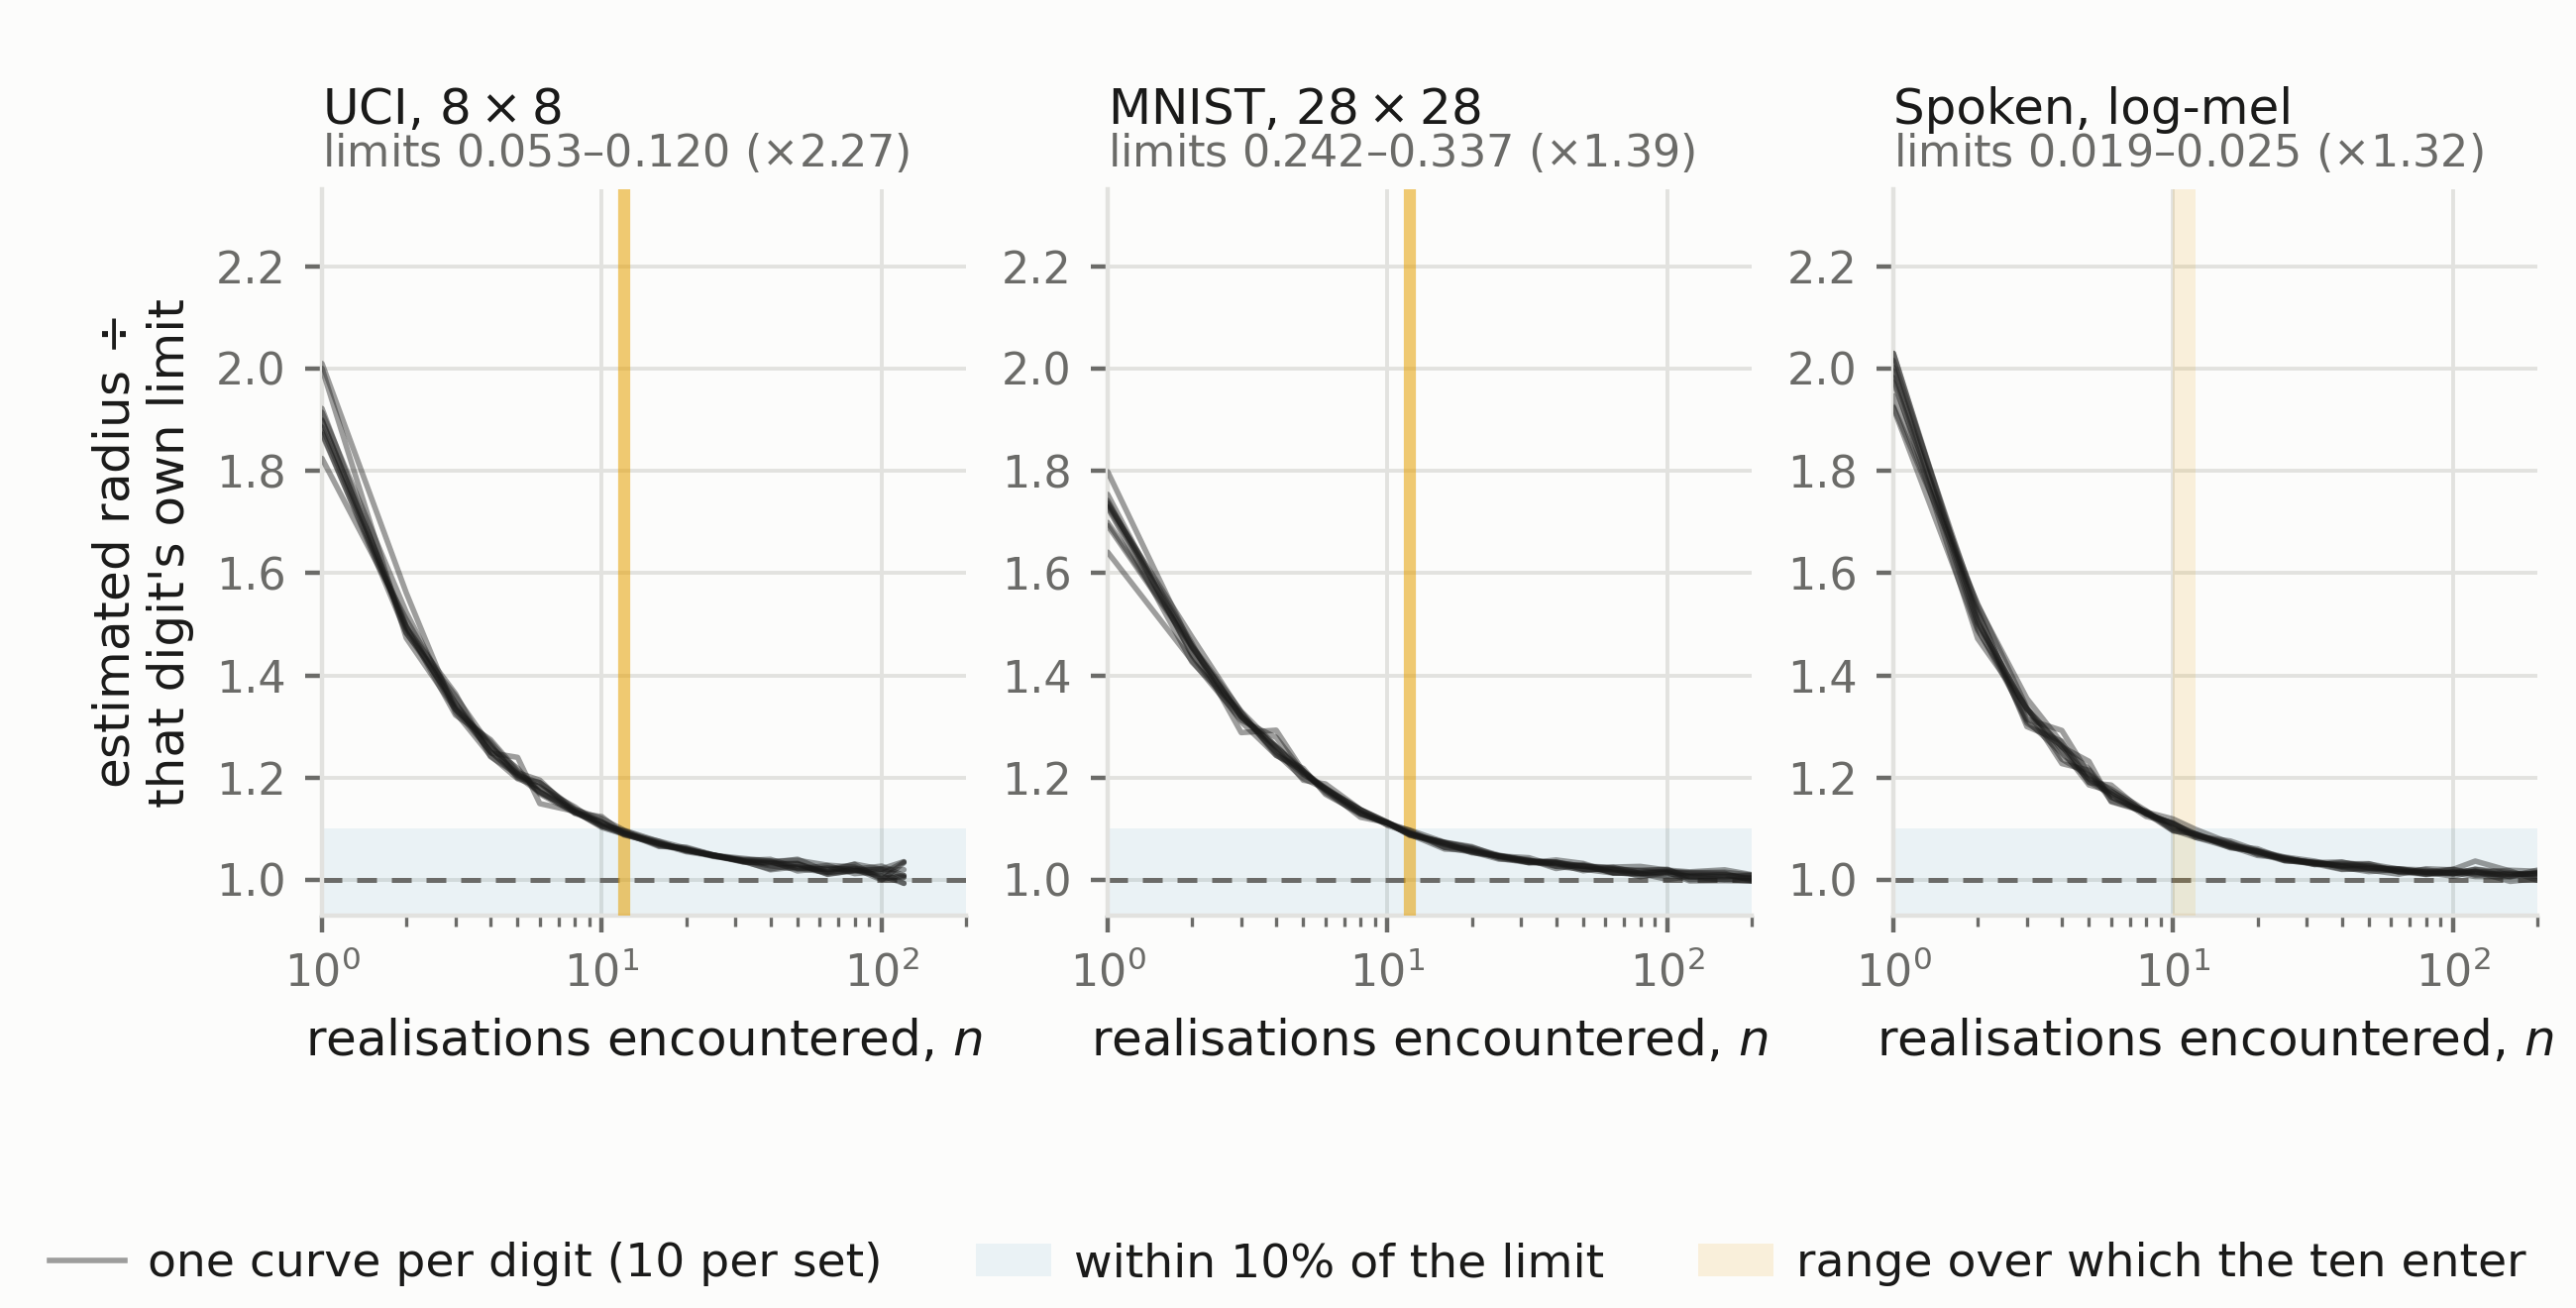
\includegraphics[width=\textwidth]{fig_digits_per_class.png}
\caption{\small The ten concepts of each digit set, one grey curve each. Each
curve is the radius an observer estimates for that digit after $n$ encounters,
measured on realisations it has not seen, divided by \emph{that digit's own}
limiting radius; the division is what puts ten quantities of different size on
one axis and it does not change any curve's shape. The blue band is $\pm10\%$
of the limit; the orange mark spans the sample sizes at which the ten enter it
and stay, and is drawn as a line in the two panels where all ten enter at the
same $n$. Each panel's second line carries what the division removes --- the
spread of the ten limits, which is a property of the concepts and is not
small, a factor of $2.27$ across the ten UCI digits against $1.39$ across
MNIST and $1.32$ across the spoken set. Every limit is reported individually
in Table~\ref{tab:digits-per-class}.}
\label{fig:digits-per-class}
\end{figure}

The answer is the first case, and it is more uniform than we expected. Across
all thirty concepts --- ten digits in three sets, two modalities --- every one
enters ten per cent of its own limit at $n=10$ or $n=12$, and five per cent at
$n=20$ or $n=25$. There is no straggler and no concept that fails to settle.
In two of the three sets all ten cross at the same grid point.

What is \emph{not} uniform is how large the classes are, and
Table~\ref{tab:digits-per-class} puts the two facts side by side.

\begin{table}[!htbp]\centering\small
\fitwidth{\begin{tabular}{lrrrrrr}
\toprule
& \multicolumn{2}{c}{UCI $8\times8$} & \multicolumn{2}{c}{MNIST $28\times28$} & \multicolumn{2}{c}{Spoken (FSDD)} \\
\cmidrule(lr){2-3}\cmidrule(lr){4-5}\cmidrule(lr){6-7}
digit & limit & $n_{10\%}$ & limit & $n_{10\%}$ & limit & $n_{10\%}$ \\
\midrule
0 & 0.0526 & 12 & 0.2416 & 12 & 0.0201 & 12 \\
1 & 0.1195 & 12 & 0.2427 & 12 & 0.0211 & 10 \\
2 & 0.1005 & 12 & 0.2968 & 12 & 0.0186 & 12 \\
3 & 0.0872 & 12 & 0.2722 & 12 & 0.0212 & 12 \\
4 & 0.0996 & 12 & 0.2938 & 12 & 0.0230 & 12 \\
5 & 0.1057 & 12 & 0.3367 & 12 & 0.0245 & 12 \\
6 & 0.0671 & 12 & 0.2673 & 12 & 0.0198 & 12 \\
7 & 0.1022 & 12 & 0.2816 & 12 & 0.0232 & 10 \\
8 & 0.0961 & 12 & 0.2579 & 12 & 0.0224 & 12 \\
9 & 0.1053 & 12 & 0.2683 & 12 & 0.0205 & 10 \\
\bottomrule
\end{tabular}
% limit = the radius over every realisation of that concept.
% n_10% = smallest n after which the estimate stays within
%   ten per cent of that limit; same criterion as the body.
}
\caption{\small Per concept: the limiting radius, and the smallest $n$ after
which the estimate stays within ten per cent of it. Limits are radii in each
representation's own metric, so the columns are comparable within a set and
not across sets.}
\label{tab:digits-per-class}
\end{table}

The ten UCI limits run from $0.0526$ to $0.1195$, a factor of $2.27$; the MNIST
limits differ by $1.39$ and the spoken ones by $1.32$. A written $0$ is a
smaller region than a written $1$ by more than a factor of two under the same
observable, and both are fixed after the same dozen encounters. That is the
paper's separation stated at the level of a single concept: \textbf{the size of
a class is a property of that class, and the schedule on which an observer
learns its size is not}. The first varies by more than a factor of two inside
one dataset; the second varies by one grid step across three datasets and two
senses.

One caution about what this is. It is a decomposition of the body's
measurement and not an independent test of it --- same estimator, same
protocol, same run, the aggregate curves of Section~\ref{sec:results} are these
curves averaged. It answers the question of whether the aggregate conceals a
mixture, which it does not, and it answers nothing else.

\section{Synthetic Generator for the Electromechanical Domain}
\label{app:gen_electromechanical}

This appendix details the deterministic generator used to construct synthetic 
electromechanical traces.  
Its purpose is not to reproduce the detailed physics of any specific machine, 
but to create a compact, bounded-variability functional manifold with the 
characteristic morphology observed in real electromechanical actuation: an 
initial idle regime, a fast high-amplitude transient, a quasi-stationary 
plateau, and a terminal decay.  
The generator produces only the AC waveform.  
The RMS envelopes used in the experiments are computed from these synthetic AC 
signals using exactly the same sliding-window RMS operator applied to the 
real electromechanical data.  
This guarantees that the synthetic and real RMS traces are directly comparable 
and that no domain-specific preprocessing differences bias the geometric 
analysis.

\subsection{Time segmentation}

Let the actuation interval $[0,T]$ be partitioned into the ordered times
\[
0 < t_{\mathrm{idle}} < t_{\mathrm{peak}} < t_{\mathrm{end}} <
t_{\mathrm{cut}} < t_{\mathrm{step}} < t_{\mathrm{ramp}} < T,
\]
defined from a compact parameter vector
\[
\theta = (A_{\mathrm{idle}}, A_{\mathrm{peak}}, A_{\mathrm{plateau}}, 
          \Delta t_{\mathrm{idle}}, \Delta t_{\mathrm{rise}},
          \Delta t_{\mathrm{decay}}, t_{\mathrm{cut}},
          \Delta t_{\mathrm{step}}, \Delta t_{\mathrm{ramp}}) \in \Theta.
\]
The boundaries are
\[
\begin{aligned}
t_{\mathrm{idle}} &= \Delta t_{\mathrm{idle}}, \\
t_{\mathrm{peak}} &= t_{\mathrm{idle}} + \Delta t_{\mathrm{rise}},\\
t_{\mathrm{end}}  &= t_{\mathrm{peak}} + \Delta t_{\mathrm{decay}},\\
t_{\mathrm{step}} &= t_{\mathrm{cut}} + \Delta t_{\mathrm{step}},\\
t_{\mathrm{ramp}} &= t_{\mathrm{step}} + \Delta t_{\mathrm{ramp}}.
\end{aligned}
\]
All parameters vary in bounded ranges, so $\Theta$ is compact.

\subsection{Deterministic envelope}

A piecewise envelope $e_\theta(t)$ is constructed as follows.

\paragraph{Idle and micro-bump.}
A baseline amplitude $A_{\mathrm{idle}}$ is maintained on $[0,t_{\mathrm{idle}})$, 
with a small pre-transient bump of the form
\[
b(t) = A_{\mathrm{bump}}
       \sin \bigl( \varphi(t) \bigr), \qquad 
\varphi(t) \in [0,\pi/2],
\]
applied over a short interval ending at $t_{\mathrm{idle}}$.

\paragraph{Fast rise.}
On $[t_{\mathrm{idle}}, t_{\mathrm{peak}})$ the envelope increases linearly from 
the end of the bump to the peak amplitude $A_{\mathrm{peak}}$:
\[
e_\theta(t)
  = \text{lin}\bigl(t;\, A_{\mathrm{bump,end}},\, A_{\mathrm{peak}}\bigr).
\]

\paragraph{Shoulder and drop.}
A short plateau around $A_{\mathrm{peak}}$ is followed by a linear decrease to
\[
A_{\mathrm{drop}} = \alpha\,A_{\mathrm{peak}},\qquad \alpha \in (0,1),
\]
over a compact-duration window.

\paragraph{Decay to plateau.}
Over $[t_{\mathrm{shoulder,end}}, t_{\mathrm{end}})$ the envelope decays 
linearly to the plateau amplitude $A_{\mathrm{plateau}}$.

\paragraph{Fast cutoff and slow decay.}
At $t_{\mathrm{cut}}$ a fast drop occurs to
\[
A_{\mathrm{step}} = \beta A_{\mathrm{plateau}}, \qquad \beta \in (0,1),
\]
followed by a slow exponential decay:
\[
e_\theta(t) = A_{\mathrm{step}} e^{-k(t - t_{\mathrm{step}})}, 
\qquad t_{\mathrm{ramp}} \le t \le T,
\]
with $k>0$ bounded.

\subsection{AC carrier and observable waveform}

The synthetic observable is the full AC waveform
\[
x_\theta(t)
  = e_\theta(t)\,\sin(2\pi f_{\mathrm{ac}} t + \phi)
    + \eta_\theta(t),
\]
where:
\begin{itemize}
\item $f_{\mathrm{ac}}$ is the AC carrier frequency,
\item $\phi$ is a bounded phase,
\item $\eta_\theta(t)$ is a bounded perturbation term consisting of:
  \[
  \eta_\theta(t)
    = \eta^{\mathrm{white}}_\theta(t)
    + \eta^{\mathrm{mult}}_\theta(t)
    + \eta^{\mathrm{OU}}_\theta(t),
  \]
  combining small white noise, multiplicative amplitude-dependent noise,  
  and a temporally correlated Ornstein–Uhlenbeck component.
\end{itemize}

\subsection{RMS computation}

No RMS envelope is generated analytically.  
Instead, the RMS signal used for geometric analysis is computed directly from 
$x_\theta(t)$ using the same sliding-window RMS operator applied to the 
real electromechanical data.  
This preserves complete methodological consistency between real and synthetic 
signals and prevents introducing artefacts from manual RMS design.

\subsection{Compactness}

Since $\Theta$ is compact and $\theta \mapsto x_\theta(\cdot)$ is continuous in 
the supremum norm, the synthetic manifold
\[
\mathcal{M}_{\mathrm{elec}}
 = \{ x_\theta : \theta \in \Theta \}
\]
is uniformly bounded and equicontinuous, hence relatively compact in
$C^0([0,T])$; being bounded, it admits a finite Hausdorff radius.

\subsection*{Implementation} 

A reference implementation of this generator, including the AC waveform, noise 
components, and RMS computation pipeline, are available in the repository
associated with this work.


\section{Synthetic Generator for the Electrochemical Domain}
\label{app:gen_battery}
\subsection{Electrochemical discharge structure}

Battery discharge under fixed load conditions produces voltage curves with
characteristic properties:
\begin{itemize}
    \item monotonic or quasi-monotonic decay,
    \item smooth curvature with a knee region,
    \item bounded voltage range determined by chemistry and operating limits,
    \item absence of high-frequency transients.
\end{itemize}

These properties reflect deterministic electrochemical constraints governed by
reaction kinetics, internal resistance, and diffusion processes.

\subsection{Parameterisation}

Each discharge curve is parameterised by a vector
\[
\theta = (V_0, V_{\min}, \alpha, \beta, t_k, \gamma, \varepsilon) \in \Theta,
\]
where:
\begin{itemize}
    \item $V_0$ is the initial voltage,
    \item $V_{\min}$ is the cutoff voltage,
    \item $\alpha$ controls early-stage decay,
    \item $\beta$ controls mid-stage curvature,
    \item $t_k$ defines the knee location,
    \item $\gamma$ controls terminal tapering,
    \item $\varepsilon$ bounds smooth perturbations.
\end{itemize}

All parameters vary within bounded intervals, so $\Theta$ is compact.

\subsection{Deterministic discharge model}

The nominal discharge envelope is defined as
\[
v_\theta(t) =
V_{\min}
+ (V_0 - V_{\min})
\exp\!\left(
- \alpha t
- \beta \max(0, t - t_k)^2
\right),
\qquad t \in [0,T].
\]

This formulation captures:
\begin{itemize}
    \item an initial exponential decay,
    \item a curvature increase around the knee,
    \item a smooth approach to the cutoff voltage.
\end{itemize}

\subsection{Smooth bounded perturbations}

To account for structured variability while preserving continuity, we add a
bounded smooth perturbation:
\[
\eta_\theta(t)
= \varepsilon \sum_{j=1}^{J} c_j(\theta)\,\psi_j(t),
\]
where:
\begin{itemize}
    \item $\psi_j$ are fixed smooth basis functions on $[0,T]$,
    \item $c_j(\theta)$ are bounded continuous coefficients,
    \item $J$ is finite.
\end{itemize}

The final observable voltage curve is
\[
x_\theta(t) = v_\theta(t) + \eta_\theta(t).  
\]

\subsection{Compactness of the electrochemical manifold}

The synthetic electrochemical manifold is defined as
\[
\mathcal{M}_{\mathrm{bat}}
= \{\, x_\theta(\cdot) : \theta \in \Theta \,\}
\subset C^0([0,T]).
\]

Since $\Theta$ is compact and the map
$\theta \mapsto x_\theta(\cdot)$ is continuous in the supremum norm, the image
$\mathcal{M}_{\mathrm{bat}}$ is compact by the standard image-of-compact-is-compact
argument. Consequently, the electrochemical perceptual manifold admits a finite
Hausdorff radius.

\subsection{Status of synthetic evaluation}

The electrochemical domain is empirically validated in this work using real
NASA battery discharge curves, as reported in Section~\ref{sec:results-battery}. The synthetic
electrochemical generator described above is included only as a theoretical
reference model illustrating how bounded discharge families may arise from a
compact parameterisation.
We do not use this synthetic generator in the reported battery experiments.
Unlike the point-machine and ECG cases, where synthetic generators are used to
compare real and simulated manifold saturation, the battery results in this work
are based exclusively on real discharge data. A more detailed physics-aware
battery simulator is left for future work.

%--------------------------------------------------------
% ECG GENERATOR
%--------------------------------------------------------

\section{Synthetic Generators for the ECG Domain}
\label{app:gen_ecg}

This appendix details the synthetic generators used to construct compact
functional manifolds representative of electrocardiogram (ECG) signals.
The goal is not to reproduce the full electrophysiological complexity of
cardiac dynamics, but to generate bounded, continuous families of waveforms
with stereotyped heartbeat morphology suitable for geometric analysis.

Two generators of increasing abstraction are considered:
(i) a dynamical ECG generator based on the McSharry model, and
(ii) a purely morphological Gaussian generator.
Both produce continuous signals on a fixed time interval and induce compact
perceptual manifolds in $C^0([0,T])$.

\subsection{Common preprocessing and representation}

All synthetic ECG signals are generated on a fixed interval $[0,T]$ centered
around the R-peak. Signals are resampled onto a uniform temporal grid and
normalised in amplitude using the same preprocessing pipeline applied to real
ECG data. This guarantees that synthetic and real signals are directly
comparable under the same metric geometry.

\subsection{McSharry dynamical ECG generator}

The McSharry generator~\citep{mcsharry2003dynamical} models ECG signals using a
low-dimensional nonlinear dynamical system designed to produce a stereotyped
P--QRS--T morphology. While simplified, this model captures the gross temporal
structure of cardiac cycles.

\subsubsection{Parameterisation}

Each realisation is determined by a parameter vector
\[
\theta = (A_P, A_Q, A_R, A_S, A_T;\;
          t_P, t_Q, t_R, t_S, t_T;\;
          \sigma_P, \sigma_Q, \sigma_R, \sigma_S, \sigma_T;\;
          \varepsilon)
\in \Theta,
\]
where:
\begin{itemize}
    \item $A_k$ control the amplitudes of the P, Q, R, S, and T components,
    \item $t_k$ define their temporal locations,
    \item $\sigma_k$ control their temporal widths,
    \item $\varepsilon$ bounds smooth perturbations.
\end{itemize}
All parameters vary within bounded intervals, so $\Theta$ is compact.

\subsubsection{Deterministic waveform construction}

The nominal ECG waveform is constructed as a superposition of smooth
components:
\[
f_\theta(t) = \sum_{k \in \{P,Q,R,S,T\}}
A_k \exp\!\left( -\frac{(t - t_k)^2}{2\sigma_k^2} \right).
\]

Additional smooth perturbations are added to account for structured variability:
\[
\eta_\theta(t)
= \varepsilon \sum_{j=1}^{J} c_j(\theta)\,\psi_j(t),
\]
where $\psi_j$ are fixed smooth basis functions on $[0,T]$ and $J$ is finite.

The final observable signal is
\[
x_\theta(t) = f_\theta(t) + \eta_\theta(t).
\]

\subsubsection{Compactness}

Since $\Theta$ is compact and the map
$\theta \mapsto x_\theta(\cdot)$ is continuous in the supremum norm, the
synthetic ECG manifold generated by the McSharry model,
\[
\mathcal{M}_{\mathrm{ECG}}^{\mathrm{McS}}
= \{ x_\theta : \theta \in \Theta \},
\]
is uniformly bounded and equicontinuous, hence relatively compact in
$C^0([0,T])$; being bounded, it admits a finite Hausdorff radius.

\subsection{Gaussian morphological ECG generator}

To decouple geometric properties from physiological modelling assumptions, we
also consider a purely morphological ECG generator based on Gaussian
components. This generator ignores cardiac dynamics entirely and retains only
coarse waveform structure.

\subsubsection{Parameterisation}

Each synthetic beat is defined by
\[
\theta = (a_1,a_2,a_3;\; t_1,t_2,t_3;\;
          \sigma_1,\sigma_2,\sigma_3;\; b,\; \varepsilon)
\in \Theta,
\]
where:
\begin{itemize}
    \item $a_k$ control the amplitudes of three dominant excursions
          (e.g.\ P/QRS/T),
    \item $t_k$ define their temporal locations,
    \item $\sigma_k$ control their widths,
    \item $b$ defines a baseline offset,
    \item $\varepsilon$ bounds smooth perturbations.
\end{itemize}
All parameters are bounded, so $\Theta$ is compact.

\subsubsection{Deterministic waveform}

The deterministic component is
\[
f_\theta(t)
= b + \sum_{k=1}^{3}
a_k \exp\!\left( -\frac{(t - t_k)^2}{2\sigma_k^2} \right),
\]
with a smooth perturbation term $\eta_\theta(t)$ defined as in the previous
section. The observable waveform is
\[
x_\theta(t) = f_\theta(t) + \eta_\theta(t).
\]

\subsubsection{Compactness}

As before, compactness of $\Theta$ and continuity of the construction imply
that the Gaussian ECG manifold
\[
\mathcal{M}_{\mathrm{ECG}}^{\mathrm{Gauss}}
= \{ x_\theta : \theta \in \Theta \}
\]
is uniformly bounded and equicontinuous, hence relatively compact in
$C^0([0,T])$; being bounded, it admits a finite Hausdorff radius.

\subsection{Remarks on realism and geometry}

Neither generator is intended to produce physiologically accurate ECG signals.
The McSharry model captures coarse heartbeat dynamics but omits many biological
details, while the Gaussian generator is purely morphological.

Both are nonetheless compact by construction --- bounded parameters, continuous
by design, and proved compact above --- and their estimates settle on the same
schedule as the measured recordings. No measurement here could have found them
non-compact, so this is an illustration of the framework's reach and not
evidence for it: what it shows is that the \emph{schedule} does not require
physiological realism. The geometry does differ, and
Section~\ref{sec:ecg-sim-geometry} reports how.

\subsection*{Implementation}

Reference implementations of both ECG generators, together with preprocessing
and resampling routines identical to those applied to real ECG data, are
provided in the repository associated with this work.



\section{Padding and Room Tone Experiment for Spoken Digits}\label{app:padding}
\subsection{A domain that was not receiving this rule}
\label{sec:spoken-duration}

The rule stated above --- every signal resampled onto a uniform temporal grid
--- is a quotient by duration, and the physical domains receive it. The
spoken-digit loader did not apply it. It zero-padded every recording to a fixed
one second, and the log-mel spectrogram of a zero-padded tail is exactly the
floor value, identical in every recording: in this set the median recording
carries fifty of its hundred and one frames as padding, and $55\%$ of all
frames are that constant. More than half of every vector therefore encoded one
fact only, that the recording was shorter than a second. After $\ell_2$
normalisation a large shared constant drags every cosine distance towards zero,
within class and between classes alike, and the within-class median gives it
away: $0.025$ for the padded spoken set against $0.47$ for MNIST. It is the
same defect that makes amplitude-only normalisation inappropriate for battery
discharge, where a constant of ${\sim}3.3$~V carries ${\sim}0.2$~V of signal.

The correction brings this domain under the rule the others already follow: the
padding frames are dropped and what remains is resampled onto the same number
of frames the representation already had. It introduces no threshold ---
padding frames equal the floor to floating-point equality, so they are
identified and not estimated --- and no new constant, since the output has the
dimension of the input.

The correction is not a licence taken after the fact. It follows from a group
this paper had already declared for this domain before measuring: the benign
variation of a spoken digit is \emph{who is speaking and how fast}. Declaring
the speaker benign declares away the only thing that would make duration
readable, because a duration is informative relative to \emph{that speaker's}
rate and not in the absolute. The measurement agrees. Spoken digits do differ
in length in the direction one expects --- \emph{two} averages $401$~ms and
\emph{seven} $472$~ms --- but the spread of the class means is $38$~ms while the
spread within a single class, across speakers, is $130$~ms. Separability on
duration alone is $0.531$, against a chance value of $0.5$. Under a declared
speaker group, duration carries almost no information about which digit was
said.

Two further points belong here. Both arms are reported: the padded numbers
appear in Contribution~5 and in Table~\ref{tab:separability}, the cached
observable remains the raw padded representation, and the quotient is applied
on top of it, so either can be recomputed. And the correction leaves the
convergence measurement --- the quantity this paper's central claim is about ---
unchanged to the last digit reported: the estimate enters ten per cent of its
limit at $n=12$ and five per cent at $n=25$, before and after. Only the value of
the limiting radius moves, as it must when the representation changes. Had the
quotient been buying the central result, the central result would have moved.

\subsection{The cost of the padding}

It is natural to read the defect as the shared constant alone, and to expect
that filling the pad with something varied would repair it. We tested that:
replacing each recording's padding frames with frames drawn from its own
quietest real frames --- its room tone rather than the numerical floor. It
does dissolve the shared component, and the within-class median nearly doubles,
from $0.024$ to $0.044$. It does not recover separability, which stays at
$0.557$ against $0.554$ for the constant pad.

So the cost was not the constant. It was that a fixed window compares
incommensurable positions: with padding, frame thirty of a short utterance is
already silence while frame thirty of a long one is mid-vowel, and the metric
is asked to compare them. What buys separability is placing comparable events
at comparable positions, which is what resampling onto a common grid does and
what the physical domains have always received. This control is a proxy: the
noise was synthesised in the log-mel domain and independently per recording,
whereas real room tone would be correlated within a speaker and a session.

\subsection{A declaration open to dispute}

None of this makes the declaration obviously correct. A reader who is
interested in a single speaker, where rate is fixed and duration therefore is
informative, would be right to keep it, and would be describing a different
observer from the one declared here. We declare the speaker and the rate benign,
we report what that declaration bought, and we report the arm without it. This
is the ordinary situation the scope condition of Section~\ref{sec:scope}
describes: the group is declared, the declaration is contestable, and its
consequences are measured rather than assumed.


\section{Algorithm for Incremental Radius Estimation}\label{app:algorithm}
\begin{algorithm}[H]
\caption{Incremental Estimation of the Perceptual Radius}
\begin{algorithmic}[1]

\Require Stream of realisations $(x_1, x_2, \dots)$, reference $x_0$
\State Initialize vector index $\mathcal{I} \gets \emptyset$
\State $\hat r_0 \gets 0$

\For{$n = 1,2,\dots$}

    \State Insert $x_n$ into index: $\mathcal{I} \gets \mathcal{I} \cup \{x_n\}$
    
    \State Compute distance to reference:
    \[
       d_n = \|x_n - x_0\|_\infty
    \]
    
    \State Update empirical radius:
    \[
        \hat r_n = \max(\hat r_{n-1}, d_n)
    \]
    
    \State Optionally return early-warning signals:
    \[
    \text{if } d_n > \hat r_{n-1} + \delta 
       \Rightarrow \text{new variability detected}
    \]
    
\EndFor

\State \Return $\hat r_n$, and the sample size at which it entered its band
\end{algorithmic}
\end{algorithm}


\section{Domain-by-Domain Hypotheses Statements}\label{app:hypotheses}



Section~\ref{sec:hypotheses} stated H1, H2 and H3 as claims about the world
rather than as lemmas, and said that the risk of the argument lives there. A
claim about the world that is never attached to a particular world costs
nothing, so we attach them here. Each declaration names the observable, says
what bounds it, says what bounds its rate of change, and says where the
observable is known or suspected not to resolve. Each is falsifiable in the
same way: exhibit two realisations that the domain calls different and that the
declared observable does not separate, or one that leaves the stated bound.

\paragraph{Railway point machine.}
\emph{Observable}: the instantaneous RMS electrical power drawn by the motor
during one manoeuvre, resampled to $160$ points and quotiented by amplitude.
\emph{H1}: the motor's rated power bounds it; a manoeuvre drawing more is a
fault, not a nominal realisation, which is the sense in which the bound is a
statement about the machine and not about the data. \emph{H2}: the assembly has
mechanical inertia and the supply finite power, so the rate of change of the
envelope is bounded; an electrical fault such as arcing has a transient faster
than the mechanism and violates this. \emph{H3}: power is one scalar projection
of a mechanical process, and after the temporal quotient it projects the
\emph{shape} of that process alone. Two manoeuvres differing in a way that does
not change the torque demanded --- a lateral adjustment within tolerance --- are
not separated by it. Neither are two that differ only in how long they take: a
throw slowed by friction and a throw at nominal speed with the same power
profile are one point under this observable. That is the sharpest falsification
available for this domain, and duration is the channel to test it with.

\paragraph{Electrocardiogram.}
\emph{Observable}: one beat from a single lead, aligned at the R peak, on $160$
points, quotiented by amplitude. \emph{H1}: cardiac transmembrane potentials
bound the surface voltage, and the recording amplifier bounds it again.
\emph{H2}: conduction velocity in cardiac tissue is finite and the recording
bandwidth is finite. \emph{H3}: a single lead is one projection of a
three-dimensional dipole, and two rhythms differing only in a direction
orthogonal to that lead are not resolved by it. This is the plainest case in
this paper of a declared observable known in advance to be incomplete ---
clinical practice uses twelve leads for exactly this reason --- and it is
declared rather than defended.

\paragraph{Battery discharge.}
\emph{Observable}: terminal voltage over a constant-current discharge,
quotiented by amplitude and offset. \emph{H1}: the electrochemistry bounds the
cell voltage between its cut-off and its fully charged value. \emph{H2}: finite
current into finite capacitance bounds the rate of change. \emph{H3}: voltage
under one declared load. Cells whose internal state differs but whose terminal
voltage under that load does not are not separated; a different discharge rate
is a different observable, not a further realisation of this one.

\paragraph{Tides.}
\emph{Observable}: water level over one lunar day ($24.8412$~h) on $128$ points,
aligned to high water, on the mean-sea-level datum, and \emph{not} normalised in
amplitude. The last is deliberate and it is a correction: min--max normalising
each day erases the spring--neap variation exactly, since it maps every day's
range to the same interval whatever that range was, and initial analyses did so and consequently reported tides as the most compact domain
studied. \emph{H1}: the
tidal range at a fixed station is bounded. \emph{H2}: the water surface responds
to a bounded astronomical forcing through a basin with a finite response time.
\emph{H3}: the level at one station resolves the local harmonic mixture but not
which constituents produce it. A storm surge enters as a violation of H1 rather
than as a realisation: the meteorological contribution is not part of the
declared astronomical process, and separating the two is what the choice of
datum and the refusal to normalise are for.

\paragraph{Solar irradiance.}
\emph{Observable}: global horizontal irradiance over $24$ hourly samples, split
by the total cloud cover the record itself reports. \emph{H1}: extraterrestrial
irradiance bounds it. \emph{H2}: \textbf{this is the weakest equicontinuity
claim in the paper, and we would rather name it than let a reader find it.} A
cloud edge crossing the sensor changes irradiance faster than an hourly grid can
represent, so H2 holds for the sampled series and is doubtful for the underlying
process. The split by cloud cover is what makes the hypothesis defensible on the
clear-sky subset and openly questionable on the overcast one, and the
measurement is consistent with that reading: the covering radius of the overcast
subset is $5.3$ times the clear-sky one. \emph{H3}: irradiance at one site under
a declared sky condition; it does not resolve which atmospheric state produced a
given profile.

\paragraph{Spoken digits.}
\emph{Observable}: a log-mel spectrogram --- $16$~kHz, $64$ mel bands, a
$400$-sample window with hop $160$ --- quotiented by duration as described in
Section~\ref{sec:spoken-duration}. \emph{H1}: the recording is bounded and the
log-mel floor bounds it below. \emph{H2}: the analysis window enforces it, since
a $25$~ms window cannot represent change faster than itself, and the vocal tract
has mechanical inertia besides. \emph{H3}: \textbf{this is the weakest resolving
claim in the paper, and unlike the others it is measured rather than argued.}
The observable resolves the geometry of one class well --- its radius converges
at $n=12$ like every other curve --- and resolves the ten classes from each other
poorly, at a separability of $0.63$ against $0.87$ for the UCI digits
(Table~\ref{tab:separability}). Both facts are reported.

\paragraph{Handwritten digits.}
\emph{Observable}: pixel intensities on an $8\times8$ or $28\times28$ lattice,
scaled to $[0,1]$ and quotiented by amplitude. Here \textbf{H1 and H2 hold by
construction and therefore carry no content}: a vector of bounded entries in a
finite-dimensional space is bounded and equicontinuous for free, and the
compactness argument delivers nothing the representation had not already
delivered. We state this rather than quietly enjoying it, because it is the
clearest illustration of the point Section~\ref{sec:hypotheses} makes about the
whole framework --- finiteness is nearly vacuous, and everything of interest is
the magnitude. \emph{H3} is the substantive hypothesis for these sets, and it is
measured: pixels resolve written digits at a separability of $0.87$ for the UCI
set and $0.75$ for MNIST.

\paragraph{The two simulators.}
The point-machine and ECG generators are not phenomena and no hypothesis is
declared for them. They are controls on the procedure: their admissible sets are
constructed by us, so H1 and H2 hold by construction and H3 is whatever the
generator was written to expose. They are included to show that the measurement
returns the same shape when the geometry is known, and for no other reason.



\section{Simulators as Procedural Controls}\label{app:simulators}
\subsubsection{Saturation of the Simulated PM Manifold}

We generated 8\,000 Monte Carlo waveforms using a physics-aware AC model.
Despite amplitude and noise differences, the simulated set follows the same
schedule: the estimate enters ten per cent of its limit at $n=12$ and five per
cent at $n=25$, against $n=12$ and $n=32$ for the measured set. It is also the
smaller of the two by covering number, $4.0 \pm 0.1$ exemplars against
$4.8 \pm 0.5$.

The generator is compact by construction --- bounded parameters, continuous by
design, and proved compact in \ref{app:gen_electromechanical} --- so
that is not what the agreement shows. What it shows is that the schedule
survives replacing the mechanism with a bounded parameterisation of its
envelope, which is what makes the simulator usable as a control on the
procedure rather than as further evidence about point machines.



% ------------------------------------------------------------
% 6.1.3 WAVEFORM MORPHOLOGY
% ------------------------------------------------------------
\subsubsection{Waveform Morphology and Simulation Coverage}

The two preceding subsections report the same measurement on the measured
machine and on the simulator, and they agree. What they do not show is whether
the simulator is producing the same \emph{shape} or merely the same statistics,
which is a question about morphology rather than about geometry.
Figure~\ref{fig:pm_waveforms} answers it by inspection: the generated envelopes
reproduce the idle--inrush--locking--idle organisation and the terminal impact
transient of the real manoeuvres. This is offered as a qualitative check on the
generator, not as evidence for any claim in this paper; the quantitative
comparison between the measured and simulated point-machine sets is in
Table~\ref{tab:saturation_summary}, where the two rows settle at $0.0268$ and
$0.0183$ and follow the same schedule.

\begin{figure}[!htbp]
\centering
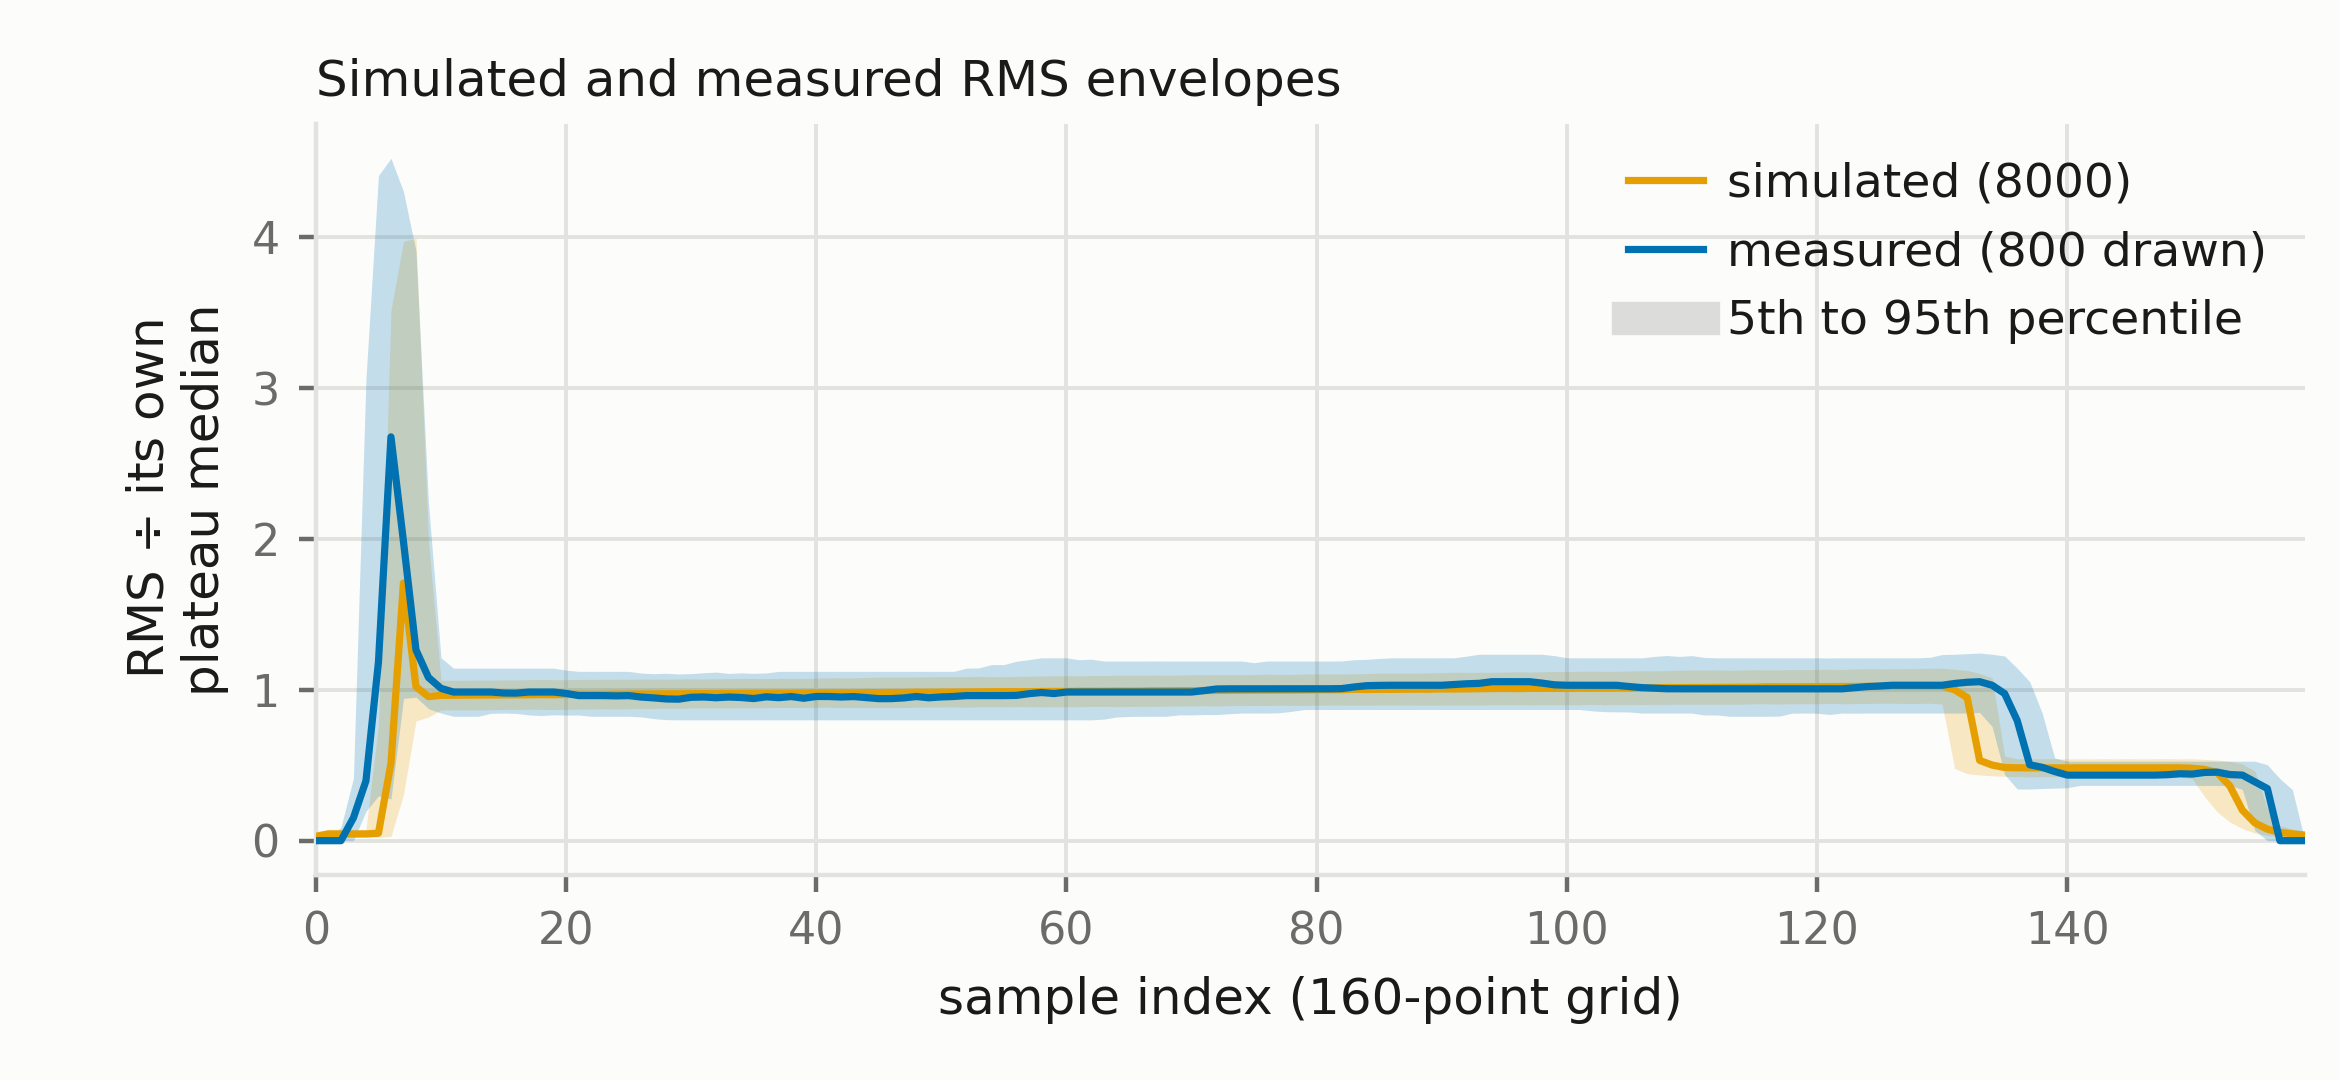
\includegraphics[width=0.90\textwidth]{pm_ac_gen_results.png}
\caption{\small
RMS instantaneous power envelopes for railway point machines, simulated
against measured. Each population is drawn as its pointwise median with the
fifth-to-ninety-fifth percentile band, and each is divided by its own plateau
median: the two are recorded in different units, and what the figure compares
is the shape. The generated envelopes reproduce the
idle--inrush--locking--idle organisation and the terminal impact transient.
They do not reproduce the inrush amplitude: the simulator's median peak
reaches $1.71$ times its plateau against $2.68$ for the measured pool. This is
a qualitative check on the generator, not evidence for any claim in this
paper, and the quantitative comparison is the one in
Table~\ref{tab:saturation_summary}.}
\label{fig:pm_waveforms}
\end{figure}

% ------------------------------------------------------------
% 6.1.4 SUMMARY
% ------------------------------------------------------------

\subsubsection{Synthetic ECG Generators}

To assess whether geometric saturation depends on accurate physiological
modelling, we analyse two synthetic ECG generators with markedly different
levels of realism. These generators are not intended to faithfully reproduce
true cardiac dynamics, but to generate bounded families of continuous waveforms
with controlled variability.

\paragraph{McSharry dynamical generator.}
We consider the well-known low-dimensional ECG model proposed by McSharry
et al.~\citep{mcsharry2003dynamical}, which generates ECG-like signals through a
nonlinear dynamical system designed to approximate the P--QRS--T morphology.
While the resulting waveforms are visually recognisable, they differ
substantially from real ECG signals in fine temporal structure, smoothness, and
relative amplitude balance.

\begin{figure}[!htbp]
\centering
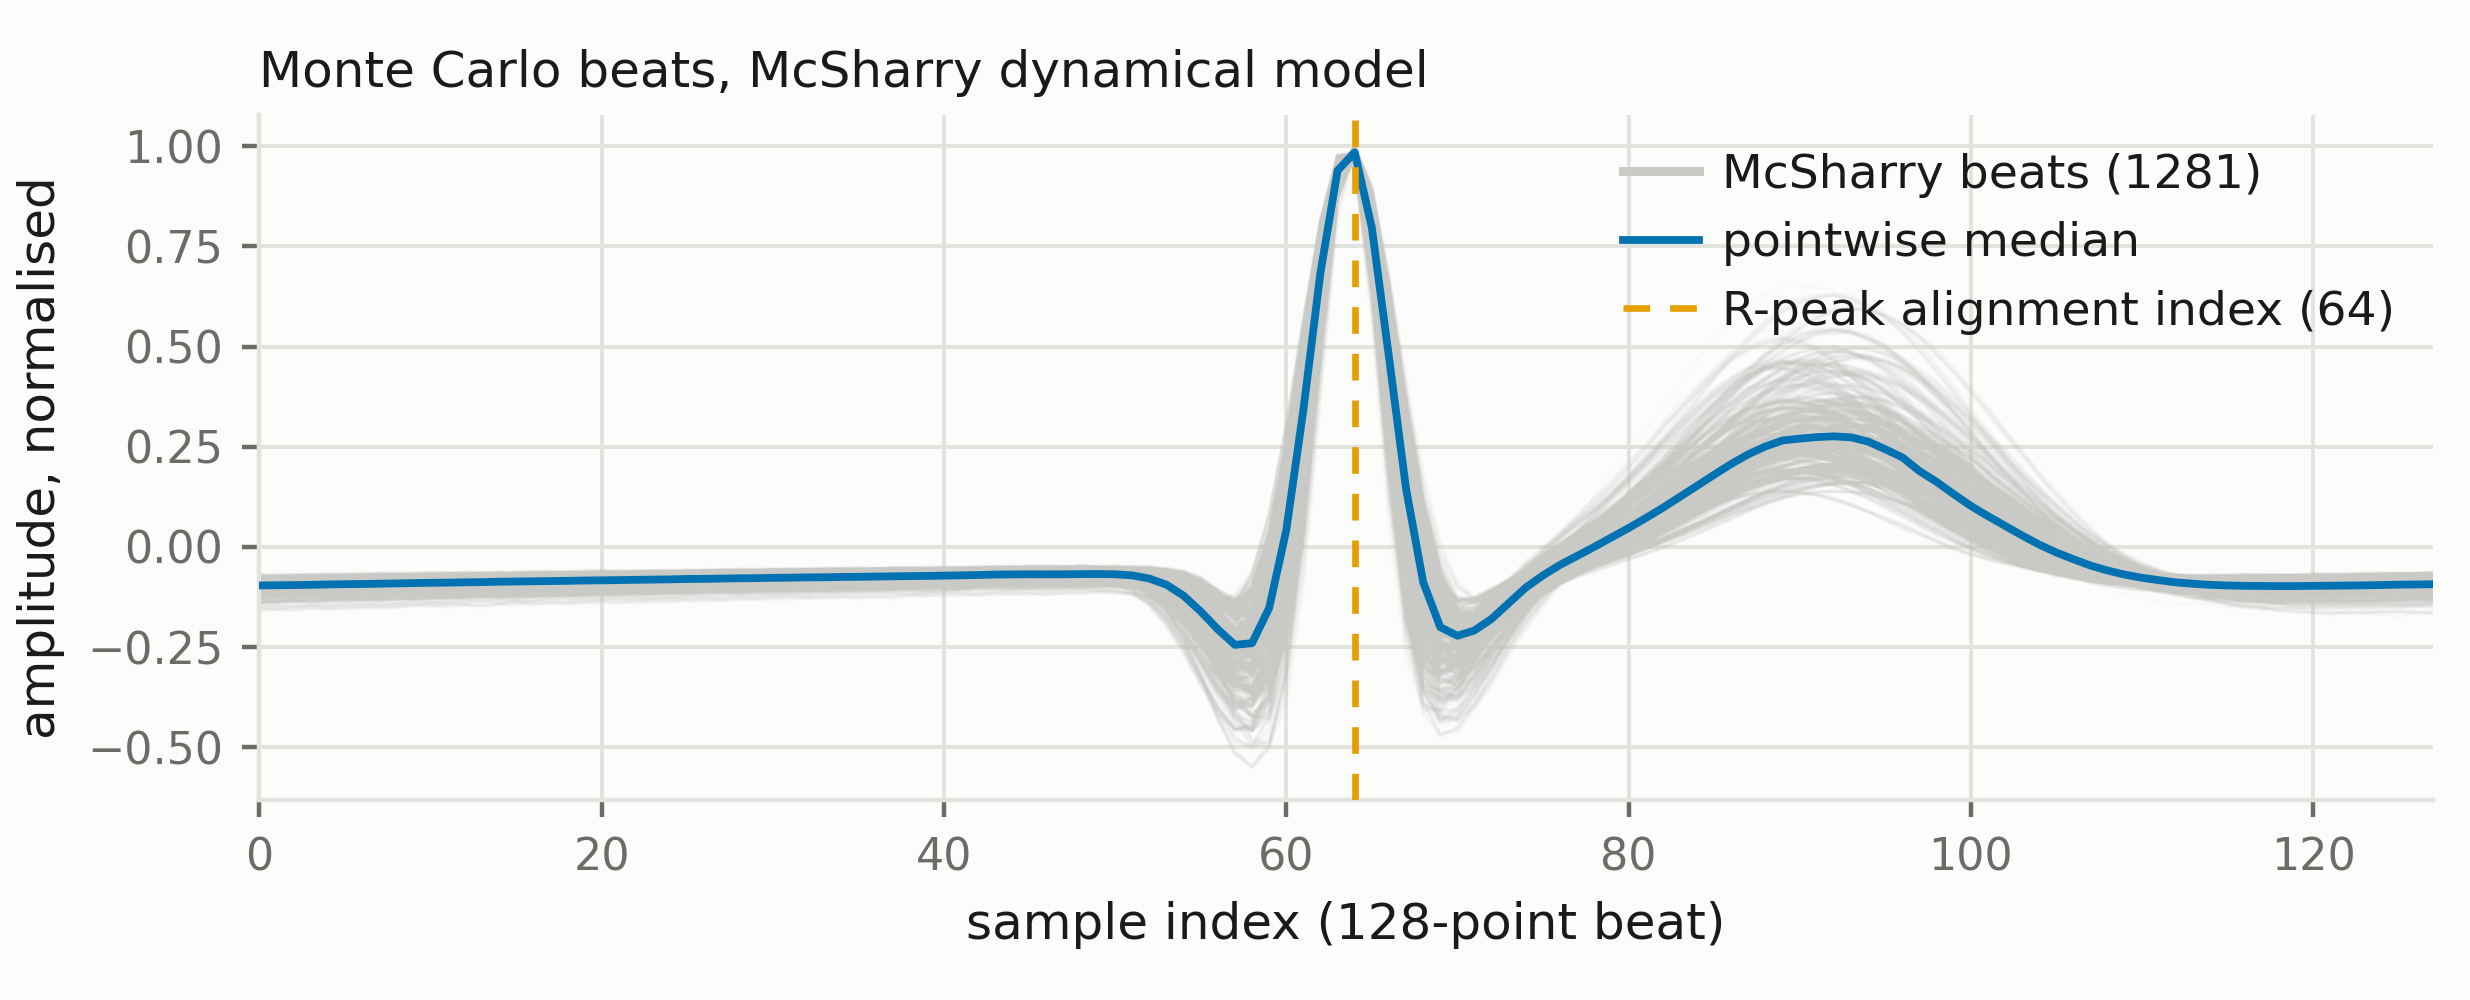
\includegraphics[width=0.95\textwidth]{mc_mcsharry_generator.png}
\caption{\small
Synthetic beats generated by the McSharry dynamical model: 1281 beats in grey,
their pointwise median in blue, and the index the beats are aligned on
(sample 64) dashed. Amplitude is normalised per beat.}
\label{fig:ecg_mchsarry_generator_examples}
\end{figure}


\paragraph{Gaussian morphological emulator.}
As a deliberately simplified baseline, we also construct a purely morphological
ECG emulator based on a superposition of Gaussian components representing the
P, QRS, and T waves, with bounded parameters and smooth perturbations. This
generator ignores electrophysiological dynamics entirely and produces visibly
idealised waveforms, yet defines a compact family of continuous signals by
construction.

\begin{figure}[!htbp]
\centering
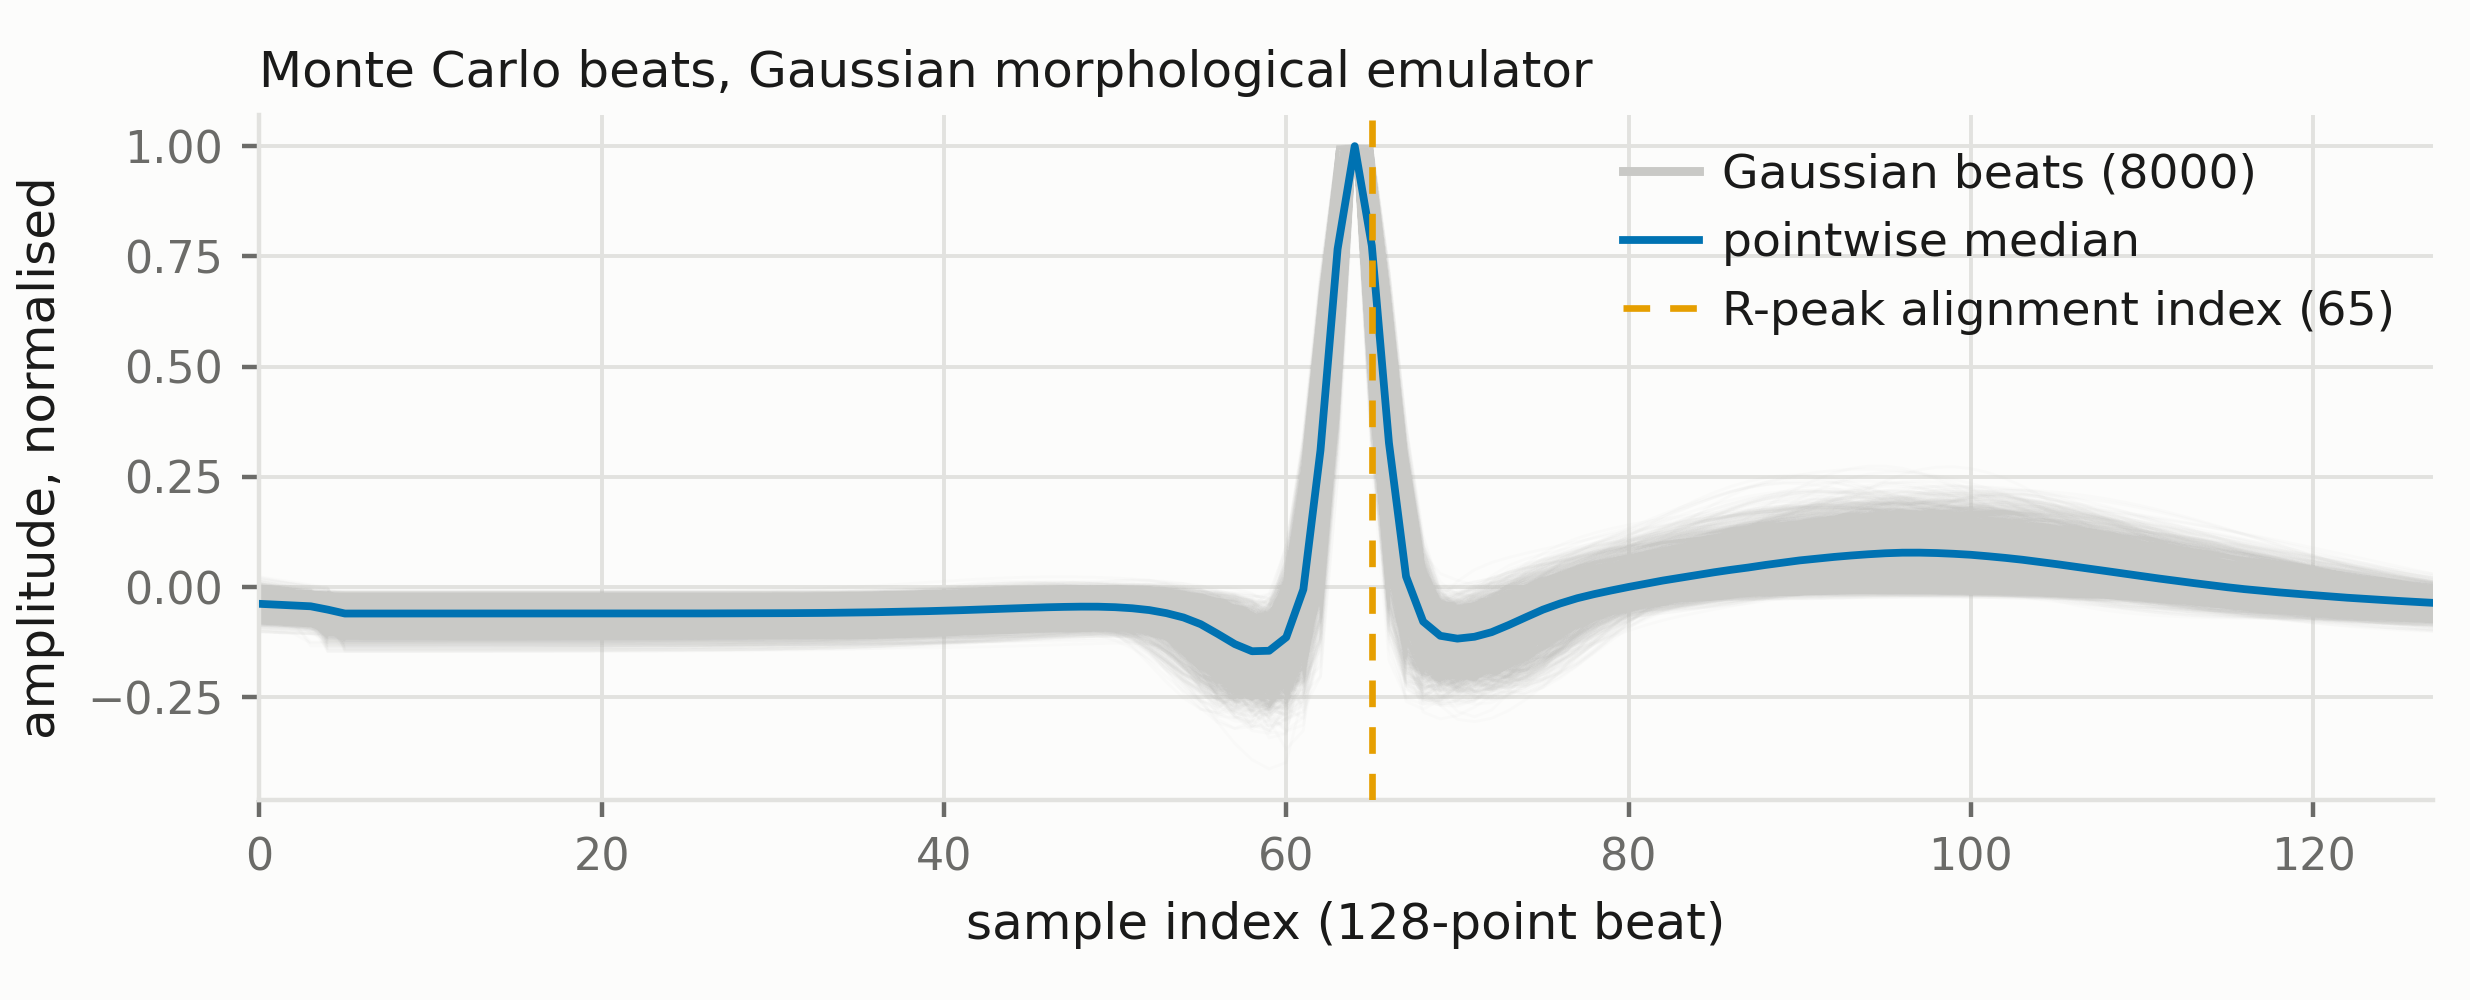
\includegraphics[width=0.95\textwidth]{ecg_gaussian_mc_gen.png}
\caption{\small
Synthetic beats produced by the Gaussian morphological emulator: 8000 beats in
grey, drawn as a two-thousand-beat sample, their pointwise median in blue, and
the alignment index (sample 65) dashed. Amplitude is normalised per beat. The
emulator ignores electrophysiological dynamics, and the comparison with
Figure~\ref{fig:ecg_mchsarry_generator_examples} is what that costs in
morphology.}
\label{fig:ecg_gaussian_generator_examples}
\end{figure}
\begin{remark}
The synthetic generators are visibly imperfect and do not reproduce fine physiological detail, yet produce bounded
families of continuous waveforms.
\end{remark}

% ------------------------------------------------------------
% 6.3.3 MCSHARRY MANIFOLD SATURATION
% ------------------------------------------------------------
\subsubsection{Saturation of the McSharry ECG Manifold}

We apply the same Monte Carlo radius estimation pipeline to the ECG signals
generated by the McSharry model. For increasing subsets
$X_n^{\mathrm{McS}}$, we compute the same radius metrics.

Despite the clear morphological discrepancies with real ECG recordings, the
synthetic manifold enters ten per cent of its limit at $n=10$ and five per
cent at $n=25$, earlier than the physiology it emulates on both counts.

Accurate physiological realism is therefore not required for early saturation.
The generator is compact by construction --- its parameters are drawn from
bounded intervals, and \ref{app:gen_ecg} proves the resulting family
compact --- so no measurement here could have found otherwise, and none is
offered as evidence that it did. What the measurement adds is the schedule, and
that the schedule is the same one the physiology follows.



% ------------------------------------------------------------
% 6.3.4 GAUSSIAN MANIFOLD SATURATION
% ------------------------------------------------------------
\subsubsection{Saturation of the Gaussian ECG Manifold}

We repeat the same analysis for the Gaussian morphological emulator. Although
this generator lacks any electrophysiological or dynamical grounding, its
parameters are bounded and the resulting signals are continuous by design.

The empirical perceptual radius again enters ten per cent of its limit early
and stays there.

The same reading applies. This generator is also compact by construction, so
its saturation is not a discovery; what it establishes is that the schedule
survives stripping the model down to bounded parameters and continuity, which
is the property the framework actually names.



% ------------------------------------------------------------
% 6.3.5 SUMMARY
% ------------------------------------------------------------
\subsubsection{Summary: Saturation Across Real and Synthetic ECG Manifolds}

Across real ECG recordings, the McSharry dynamical generator, and the simplified
Gaussian morphological emulator, we observe the same qualitative geometric
behaviour:
\begin{itemize}
    \item An observer's estimate of the radius enters ten per cent of its limit
    at $n \le 12$ in all three, and does not leave.
    \item The five per cent band separates them: $n=25$ for both generators,
    $n=160$ for the measured recordings.
    \item The measured set is the larger of the three by covering number
    ($21.0$ exemplars against $9.6$) and the \emph{lower} in intrinsic
    dimension.
\end{itemize}

Saturation occurs even when the synthetic generators fail to reproduce fine
physiological detail. Read carefully, that says less than it appears to: it
says that early saturation does not require fidelity, not that the simulated
and measured manifolds are the same object. The next subsection measures the
difference and finds it large.

\subsubsection{Dimensionality and Coverage Characteristics of the Emulator}
\label{sec:ecg-sim-geometry}

Two instruments in this paper describe the ECG generator, and they disagree in
a way that is informative rather than contradictory.

\begin{center}\small
\begin{tabular}{lrr}
\toprule
 & exemplars at its own resolution & intrinsic dimension \\
\midrule
ECG real (MIT-BIH) & $21.0 \pm 1.1$ & $2.28 \pm 0.07$ \\
ECG simulated & $9.6 \pm 0.6$ & $3.82 \pm 0.05$ \\
\bottomrule
\end{tabular}

\end{center}

The emulator needs \emph{fewer} than half the exemplars of the physiology it
emulates, and sits at a \emph{higher} intrinsic dimension. Both quantities come
from the same run at $n=600$, the first from
Table~\ref{tab:surrogates} and the second from Table~\ref{tab:dimension}.

The two readings are reconciled by what a generator is. Its parameters are
independent by construction --- amplitudes, widths and positions of the five
waves are drawn separately --- so the set it produces extends in more
directions than the measured one, and a slope fitted to its covering numbers
reports that. But each parameter is drawn over a narrow declared interval,
while a real heart varies its morphology over the range that physiology
permits, so the set is also \emph{smaller}, and a covering number at the class's
own resolution reports that. More degrees of freedom, less extent in each.

The comparison is ordinal and must stay ordinal. Section~\ref{sec:dimension-protocol}
calibrates this estimator against spheres of known dimension and shows that it
reports a lower bound; the statement licensed here is that the simulated set is
the more dimensional of the two, not that it is $1.7$ times as dimensional.

Three things follow, and the third is the one we would not have predicted.

First, early saturation is genuinely cheap: a generator with none of the
physiology reproduces it, which is what the paragraph above says and all it
says. Second, compressibility is not fidelity --- being coverable by ten
exemplars is a symptom of a small admissible set, and a set can be small
because the mechanism constrains it or because the author of the simulator
chose narrow intervals, and the covering number cannot tell those apart.
Third, and consequently, \textbf{a simulator can match the phenomenon on
saturation, fail it on dimension, and fail it in the direction of being
\emph{richer}}. The generator is not a coarser version of the heart. It is a
different object that happens to saturate, and the two measurements together
say so in a way neither says alone.

This is also the honest reading of the role these generators play here. They
are controls on the procedure --- they establish that the pipeline reports
saturation where saturation exists --- and Section~\ref{sec:scope} declares them
as such. They are not evidence about hearts, and the table above is why.


\end{document}
